%======================================================================
\Q{Problem 1 --- Smith chart reading of a mismatched line}{\m{10}}
{\color{sub}\footnotesize \yr{\textbf{79 Ch}} \gap$\cdot$\gap $Z_0 = 50\,\Omega$}

\begin{asked}{\textbf{79 Ch} \ [10]}
A lossless $50\,\Omega$ line is terminated by $75+j100\,\Omega$. Using the Smith chart find (a) $\Gamma_L$, (b) VSWR, (c) $Z_{in}$ at $0.375\lambda$ from the load, (d) the shortest length of line for which the impedance is purely resistive, and (e) the value of that resistance.
\end{asked}
\lead{Given}
\begin{itemize}
  \item $Z_L = 75.00 + j100.00\,\Omega$, $Z_0 = 50\,\Omega$.
\end{itemize}
\lead{Step 1 --- normalise and plot $z_L$}
\begin{itemize}
  \item $z_L = Z_L/Z_0 = 75.00 + j100.00$ over $50$ $=1.50 + j2.00$.
  \item Plot it where the $r = 1.50$ circle cuts the $x = +2.00$ arc; it reads $0.198\lambda$ on the WTG scale.
\end{itemize}
\lead{Step 2 --- draw the SWR circle and read (a) and (b)}
\begin{itemize}
  \item Compass on chart centre, swing a circle through $z_L$: the SWR circle. Lay its radius (dividers) on the radially scaled scales below the chart.
  \item \textbf{(a)} \emph{Refl.\ coeff.\ E or I} scale: $|\Gamma_L| = 0.644$; straight edge through $z_L$ to the \emph{angle of refl.\ coeff.} scale: $37.3^\circ$. $\boxed{\Gamma_L = 0.644\angle 37.3^\circ}$.
  \item \textbf{(b)} \emph{SWR} scale: $\boxed{S = 4.62}$, also the $r$ where the circle cuts the right-hand real axis. \textit{Check:} $(z_L-1)/(z_L+1) = 0.644\angle 37.3^\circ$, $(1+|\Gamma_L|)/(1-|\Gamma_L|) = 4.62$.
\end{itemize}
\lead{Step 3 --- rotate $0.375\lambda$ toward the generator for (c)}
\begin{itemize}
  \item $z_L$ reads $0.198\lambda$ WTG. Add $0.375\lambda$: $0.198 + 0.375 = 0.573$, and since this exceeds $0.5$, subtract half a turn $\rightarrow 0.073\lambda$.
  \item Staying on the SWR circle (the radius never changes on a lossless line), read $z_{in} = 0.27 + j0.47$.
  \item \textbf{(c)} $Z_{in} = Z_0 z_{in} = 50 \times (0.27 + j0.47) = \boxed{13.33 + j23.33\,\Omega}$.
\end{itemize}
\lead{Step 4 --- shortest purely resistive point, (d) and (e)}
\begin{itemize}
  \item $z$ is purely resistive wherever the SWR circle crosses the \textbf{horizontal axis} ($x = 0$) --- which happens twice per lap, at the voltage maximum (right) and the voltage minimum (left).
  \item Rotating clockwise from $z_L$ at $0.198\lambda$, the nearer crossing is the \textbf{voltage maximum}.
  \item \textbf{(d)} $\boxed{d = 0.052\lambda}$.
  \item \textbf{(e)} At a voltage maximum the normalised resistance is $r = S = 4.62$, so $R = 50 \times 4.617 = \boxed{230.8\,\Omega}$.
\end{itemize}

\figC{c2num_p01.png}{0.52\textwidth}
{\footnotesize\color{sub} Problem 1 --- Smith chart construction. Arcs are numbered in the order of the steps above.}

\penalty0\vspace{2pt}

%======================================================================
\Q{Problem 2 --- Single-stub shunt tuner}{\m{2}\m{8}}
{\color{sub}\footnotesize \yr{\textbf{72 Ash}} \gap$\cdot$\gap $Z_0 = 50\,\Omega$}

\begin{asked}{\textbf{72 Ash} \ [2+8]}
Design single-stub shunt tuning networks (short-circuited and open-circuited) for $Z_L = 80+j100\,\Omega$, and sketch the realisation in microstrip.
\end{asked}
\lead{Given}
\begin{itemize}
  \item $Z_L = 80.00 + j100.00\,\Omega$, $Z_0 = 50\,\Omega$.
\end{itemize}
\lead{Step 1 --- normalise and plot $z_L$}
\begin{itemize}
  \item $z_L = Z_L/Z_0 = 80.00 + j100.00$ over $50$ $=1.60 + j2.00$.
  \item Plot it where the $r = 1.60$ circle cuts the $x = +2.00$ arc; it reads $0.200\lambda$ on the WTG scale.
  \item Dividers from centre to $z_L$ (the SWR-circle radius), laid on the radially scaled scales below the chart: $|\Gamma_L| = 0.637$ on \emph{refl.\ coeff.\ E or I}, $S = 4.50$ on \emph{SWR}. \textit{Check:} $(z_L-1)/(z_L+1) = 0.637\angle 35.7^\circ$, $(1+|\Gamma_L|)/(1-|\Gamma_L|) = 4.50$.
\end{itemize}
\lead{Step 2 --- convert to admittance}
\begin{itemize}
  \item Draw the diameter through $z_L$ and read the opposite intersection --- a $\lambda/4$ half-turn. On an immittance chart read the amber grid in place and skip this step.
  \item $y_L = 1/z_L = 0.24 - j0.30$, at $0.450\lambda$ on the WTG scale (exactly $0.25\lambda$ from $z_L$).
\end{itemize}
\lead{Step 3 --- walk to the $g=1$ circle}
\begin{itemize}
  \item Swing the SWR circle (radius $|\Gamma_L| = 0.637$) through $y_L$.
  \item Rotate \textbf{clockwise} (toward the generator) to each intersection with the \textbf{$g=1$ circle}. There are always two:
  \begin{itemize}
    \item $y_1 = 1.00 + j1.65$ at $0.180\lambda$ WTG, so $d_1 = (0.500 - 0.450) + 0.180 = 0.230\lambda$.
    \item $y_2 = 1.00 - j1.65$ at $0.320\lambda$ WTG, so $d_2 = (0.500 - 0.450) + 0.320 = 0.370\lambda$.
  \end{itemize}
  \item Only the \emph{susceptance} is left to cancel: the conductance is already 1.
\end{itemize}
\lead{Step 4 --- read each stub length off the rim}
\begin{itemize}
  \item The stub must present the negative of the residual susceptance. Start at the stub's own termination and run \textbf{clockwise round the rim} until you reach that value; the arc, read on the WTG scale, is the length.
  \item \textbf{Short-circuited stub} --- start at the short-circuit point ($y=\infty$, the right of the chart):
  \begin{itemize}
    \item needs $b = -1.651$, giving $\ell_1 = 0.087\lambda$.
    \item needs $b = +1.651$, giving $\ell_2 = 0.413\lambda$.
  \end{itemize}
  \item \textbf{Open-circuited stub} --- start at the open-circuit point ($y=0$, the left of the chart):
  \begin{itemize}
    \item needs $b = -1.651$, giving $\ell_1 = 0.337\lambda$.
    \item needs $b = +1.651$, giving $\ell_2 = 0.163\lambda$.
  \end{itemize}
\end{itemize}
\lead{Answer}
\begin{tabularx}{\linewidth}{@{}L{2.6cm}X X@{}}
\toprule
\hrow \thead{Quantity} & \thead{Solution 1} & \thead{Solution 2} \\
\midrule
\textbf{Stub distance $d$} & $0.230\lambda$ & $0.370\lambda$ \\
\textbf{Line admittance} & $1.00 + j1.65$ & $1.00 - j1.65$ \\
\textbf{Short stub $\ell$} & $0.087\lambda$ & $0.413\lambda$ \\
\textbf{Open stub $\ell$} & $0.337\lambda$ & $0.163\lambda$ \\
\bottomrule
\end{tabularx}

\lead{Which to build} Solution 1 puts the stub closer to the load ($0.230\lambda$ against $0.370\lambda$), so the high-VSWR section is shorter: lower loss and wider bandwidth. Prefer it unless the layout forbids it.
\lead{Microstrip realisation}
\begin{itemize}
  \item Take FR-4, $\epsilon_r = 4.4$, $h = 1.6\text{ mm}$. Hammerstad synthesis for $50\,\Omega$ gives $W/h = 1.91$, i.e. $W = 3.06\text{ mm}$, with $\epsilon_e = 3.33$.
  \item No frequency is given, so leave the answers in wavelengths; multiply by $\lambda_g = \lambda_0/\sqrt{\epsilon_e}$ once $f$ is fixed.
  \item Draw the stubs as T-junctions off the $W$-wide main line. A shorted stub needs a plated via to the ground plane, drawn as a filled circle at the stub end.
  \item Shorten each open stub by the fringing allowance $\Delta\ell \approx 0.3h = 0.48\text{ mm}$.
\end{itemize}

\figC{c2num_p02.png}{0.55\textwidth}
{\footnotesize\color{sub} Problem 2 --- Smith chart construction. Arcs are numbered in the order of the steps above.}

\figC{c2num_p02_line.png}{0.62\textwidth}
{\footnotesize\color{sub} Problem 2 --- line diagram of the matched network: shunt stub across the line, lengths from the answer above.}

\figC{c2num_p02_ms.png}{0.92\textwidth}
{\footnotesize\color{sub} Problem 2 --- microstrip layout, top view: stubs as T-junctions off the main line, dimensions from the answer above.}

\penalty0\vspace{2pt}

%======================================================================
\Q{Problem 3 --- Single-stub shunt tuner}{\m{8}}
{\color{sub}\footnotesize \yr{\textbf{74 Bh}} \gap$\cdot$\gap $Z_0 = 50\,\Omega$}

\begin{asked}{\textbf{74 Bh} \ [8]}
A load presents $\Gamma_L = 0.5\angle 51^\circ$ on a $50\,\Omega$ line. Design single short-circuited and open-circuited shunt stubs using the Smith chart.
\end{asked}
\lead{Given}
\begin{itemize}
  \item $\Gamma_L = 0.500\angle 51.0^\circ$, $Z_0 = 50\,\Omega$ $\Rightarrow$ $Z_L = Z_0(1+\Gamma_L)/(1-\Gamma_L) = 60.42 + j62.60\,\Omega$.
\end{itemize}
\lead{Step 1 --- normalise and plot $z_L$}
\begin{itemize}
  \item $z_L = Z_L/Z_0 = 60.42 + j62.60$ over $50$ $=1.21 + j1.25$.
  \item Plot it where the $r = 1.21$ circle cuts the $x = +1.25$ arc; it reads $0.179\lambda$ on the WTG scale.
  \item Dividers from centre to $z_L$ (the SWR-circle radius), laid on the radially scaled scales below the chart: $|\Gamma_L| = 0.500$ on \emph{refl.\ coeff.\ E or I}, $S = 3.00$ on \emph{SWR}. \textit{Check:} $(z_L-1)/(z_L+1) = 0.500\angle 51.0^\circ$, $(1+|\Gamma_L|)/(1-|\Gamma_L|) = 3.00$.
\end{itemize}
\lead{Step 2 --- convert to admittance}
\begin{itemize}
  \item Draw the diameter through $z_L$ and read the opposite intersection --- a $\lambda/4$ half-turn. On an immittance chart read the amber grid in place and skip this step.
  \item $y_L = 1/z_L = 0.40 - j0.41$, at $0.429\lambda$ on the WTG scale (exactly $0.25\lambda$ from $z_L$).
\end{itemize}
\lead{Step 3 --- walk to the $g=1$ circle}
\begin{itemize}
  \item Swing the SWR circle (radius $|\Gamma_L| = 0.500$) through $y_L$.
  \item Rotate \textbf{clockwise} (toward the generator) to each intersection with the \textbf{$g=1$ circle}. There are always two:
  \begin{itemize}
    \item $y_1 = 1.00 + j1.15$ at $0.167\lambda$ WTG, so $d_1 = (0.500 - 0.429) + 0.167 \approx 0.237\lambda$.
    \item $y_2 = 1.00 - j1.15$ at $0.333\lambda$ WTG, so $d_2 = (0.500 - 0.429) + 0.333 = 0.404\lambda$.
  \end{itemize}
  \item Only the \emph{susceptance} is left to cancel: the conductance is already 1.
\end{itemize}
\lead{Step 4 --- read each stub length off the rim}
\begin{itemize}
  \item The stub must present the negative of the residual susceptance. Start at the stub's own termination and run \textbf{clockwise round the rim} until you reach that value; the arc, read on the WTG scale, is the length.
  \item \textbf{Short-circuited stub} --- start at the short-circuit point ($y=\infty$, the right of the chart):
  \begin{itemize}
    \item needs $b = -1.155$, giving $\ell_1 = 0.114\lambda$.
    \item needs $b = +1.155$, giving $\ell_2 = 0.386\lambda$.
  \end{itemize}
  \item \textbf{Open-circuited stub} --- start at the open-circuit point ($y=0$, the left of the chart):
  \begin{itemize}
    \item needs $b = -1.155$, giving $\ell_1 = 0.364\lambda$.
    \item needs $b = +1.155$, giving $\ell_2 = 0.136\lambda$.
  \end{itemize}
\end{itemize}
\lead{Answer}
\begin{tabularx}{\linewidth}{@{}L{2.6cm}X X@{}}
\toprule
\hrow \thead{Quantity} & \thead{Solution 1} & \thead{Solution 2} \\
\midrule
\textbf{Stub distance $d$} & $0.237\lambda$ & $0.404\lambda$ \\
\textbf{Line admittance} & $1.00 + j1.15$ & $1.00 - j1.15$ \\
\textbf{Short stub $\ell$} & $0.114\lambda$ & $0.386\lambda$ \\
\textbf{Open stub $\ell$} & $0.364\lambda$ & $0.136\lambda$ \\
\bottomrule
\end{tabularx}

\lead{Which to build} Solution 1 puts the stub closer to the load ($0.237\lambda$ against $0.404\lambda$), so the high-VSWR section is shorter: lower loss and wider bandwidth. Prefer it unless the layout forbids it.

\figC{c2num_p03.png}{0.55\textwidth}
{\footnotesize\color{sub} Problem 3 --- Smith chart construction. Arcs are numbered in the order of the steps above.}

\figC{c2num_p03_line.png}{0.62\textwidth}
{\footnotesize\color{sub} Problem 3 --- line diagram of the matched network: shunt stub across the line, lengths from the answer above.}

\figC{c2num_p03_coax.png}{0.89\textwidth}
{\footnotesize\color{sub} Problem 3 --- coaxial realisation, longitudinal section: each stub a coax tee off the main line; shorted stub closed by a plate, open stub left open.}

\penalty0\vspace{2pt}

%======================================================================
\Q{Problem 4 --- Single-stub shunt tuner}{\m{5}\m{3}\m{2}}
{\color{sub}\footnotesize \yr{\textbf{\texttt{81 Bh}}} \gap$\cdot$\gap $Z_0 = 100\,\Omega$}

\begin{asked}{\textbf{\texttt{81 Bh}} \ [5+3+2]}
A $100\,\Omega$ lossless line feeds a complex load $120-j160\,\Omega$. Give all design steps of a single matching stub with reasoning, and the S-matrix before and after matching.
\end{asked}
\lead{Given}
\begin{itemize}
  \item $Z_L = 120.00 - j160.00\,\Omega$, $Z_0 = 100\,\Omega$.
\end{itemize}
\lead{Step 1 --- normalise and plot $z_L$}
\begin{itemize}
  \item $z_L = Z_L/Z_0 = 120.00 - j160.00$ over $100$ $=1.20 - j1.60$.
  \item Plot it where the $r = 1.20$ circle cuts the $x = -1.60$ arc; it reads $0.315\lambda$ on the WTG scale.
  \item Dividers from centre to $z_L$ (the SWR-circle radius), laid on the radially scaled scales below the chart: $|\Gamma_L| = 0.593$ on \emph{refl.\ coeff.\ E or I}, $S = 3.91$ on \emph{SWR}. \textit{Check:} $(z_L-1)/(z_L+1) = 0.593\angle -46.8^\circ$, $(1+|\Gamma_L|)/(1-|\Gamma_L|) = 3.91$.
\end{itemize}
\lead{Step 2 --- convert to admittance}
\begin{itemize}
  \item Draw the diameter through $z_L$ and read the opposite intersection --- a $\lambda/4$ half-turn. On an immittance chart read the amber grid in place and skip this step.
  \item $y_L = 1/z_L = 0.30 + j0.40$, at $0.065\lambda$ on the WTG scale (exactly $0.25\lambda$ from $z_L$).
\end{itemize}
\lead{Step 3 --- walk to the $g=1$ circle}
\begin{itemize}
  \item Swing the SWR circle (radius $|\Gamma_L| = 0.593$) through $y_L$.
  \item Rotate \textbf{clockwise} (toward the generator) to each intersection with the \textbf{$g=1$ circle}. There are always two:
  \begin{itemize}
    \item $y_1 = 1.00 + j1.47$ at $0.175\lambda$ WTG, so $d_1 = 0.175 - 0.065 = 0.110\lambda$.
    \item $y_2 = 1.00 - j1.47$ at $0.325\lambda$ WTG, so $d_2 = 0.325 - 0.065 \approx 0.259\lambda$.
  \end{itemize}
  \item Only the \emph{susceptance} is left to cancel: the conductance is already 1.
\end{itemize}
\lead{Step 4 --- read each stub length off the rim}
\begin{itemize}
  \item The stub must present the negative of the residual susceptance. Start at the stub's own termination and run \textbf{clockwise round the rim} until you reach that value; the arc, read on the WTG scale, is the length.
  \item \textbf{Short-circuited stub} --- start at the short-circuit point ($y=\infty$, the right of the chart):
  \begin{itemize}
    \item needs $b = -1.472$, giving $\ell_1 = 0.095\lambda$.
    \item needs $b = +1.472$, giving $\ell_2 = 0.405\lambda$.
  \end{itemize}
\end{itemize}
\lead{Answer}
\begin{tabularx}{\linewidth}{@{}L{2.6cm}X X@{}}
\toprule
\hrow \thead{Quantity} & \thead{Solution 1} & \thead{Solution 2} \\
\midrule
\textbf{Stub distance $d$} & $0.110\lambda$ & $0.259\lambda$ \\
\textbf{Line admittance} & $1.00 + j1.47$ & $1.00 - j1.47$ \\
\textbf{Short stub $\ell$} & $0.095\lambda$ & $0.405\lambda$ \\
\bottomrule
\end{tabularx}

\lead{Which to build} Solution 1 puts the stub closer to the load ($0.110\lambda$ against $0.259\lambda$), so the high-VSWR section is shorter: lower loss and wider bandwidth. Prefer it unless the layout forbids it.
\lead{S-matrix before and after matching}
\begin{itemize}
  \item \textbf{Before} --- the bare load is a one-port, so $[S] = [\Gamma_L] = [0.593\angle -46.8^\circ]$, with $S = 3.91$.
  \item \textbf{After} --- the tuner makes $Z_{in} = Z_0$, so $S_{11} = S_{22} = 0$. The network is passive and reciprocal ($S_{12} = S_{21}$) and lossless, so unitarity forces $|S_{21}| = 1$:
\  \[ [S] = \begin{bmatrix} 0 & 1 \\ 1 & 0 \end{bmatrix} \quad \text{or} \quad \begin{bmatrix} 0 & e^{-j\theta} \\ e^{-j\theta} & 0 \end{bmatrix} \]
  \item Keeping the $e^{-j\theta}$ records the through-path electrical length; either form earns the marks if you say which you mean.
\end{itemize}

\figC{c2num_p04.png}{0.55\textwidth}
{\footnotesize\color{sub} Problem 4 --- Smith chart construction. Arcs are numbered in the order of the steps above.}

\figC{c2num_p04_line.png}{0.62\textwidth}
{\footnotesize\color{sub} Problem 4 --- line diagram of the matched network: shunt stub across the line, lengths from the answer above.}

\figC{c2num_p04_coax.png}{0.69\textwidth}
{\footnotesize\color{sub} Problem 4 --- coaxial realisation, longitudinal section: each stub a coax tee off the main line; a shorting plate closes each stub.}

\penalty0\vspace{2pt}

%======================================================================
\Q{Problem 5 --- Single-stub shunt tuner}{\m{10}}
{\color{sub}\footnotesize \yr{\textbf{79 Ch}} \gap$\cdot$\gap $Z_0 = 50\,\Omega$}

\begin{asked}{\textbf{79 Ch} \ [10]}
Design a single short-circuited matching stub with self-defined line and load impedances, mentioning the steps.
\end{asked}
\lead{Given}
\begin{itemize}
  \item $Z_L = 35.00 - j60.00\,\Omega$, $Z_0 = 50\,\Omega$.
  \item \added{} The paper leaves the values to the candidate; $Z_L = 35.00 - j60.00\,\Omega$ on a $50\,\Omega$ line is assumed here. Any complex load works --- the method is what earns the marks.
\end{itemize}
\lead{Step 1 --- normalise and plot $z_L$}
\begin{itemize}
  \item $z_L = Z_L/Z_0 = 35.00 - j60.00$ over $50$ $=0.70 - j1.20$.
  \item Plot it where the $r = 0.70$ circle cuts the $x = -1.20$ arc; it reads $0.346\lambda$ on the WTG scale.
  \item Dividers from centre to $z_L$ (the SWR-circle radius), laid on the radially scaled scales below the chart: $|\Gamma_L| = 0.594$ on \emph{refl.\ coeff.\ E or I}, $S = 3.93$ on \emph{SWR}. \textit{Check:} $(z_L-1)/(z_L+1) = 0.594\angle -68.8^\circ$, $(1+|\Gamma_L|)/(1-|\Gamma_L|) = 3.93$.
\end{itemize}
\lead{Step 2 --- convert to admittance}
\begin{itemize}
  \item Draw the diameter through $z_L$ and read the opposite intersection --- a $\lambda/4$ half-turn. On an immittance chart read the amber grid in place and skip this step.
  \item $y_L = 1/z_L = 0.36 + j0.62$, at $0.096\lambda$ on the WTG scale (exactly $0.25\lambda$ from $z_L$).
\end{itemize}
\lead{Step 3 --- walk to the $g=1$ circle}
\begin{itemize}
  \item Swing the SWR circle (radius $|\Gamma_L| = 0.594$) through $y_L$.
  \item Rotate \textbf{clockwise} (toward the generator) to each intersection with the \textbf{$g=1$ circle}. There are always two:
  \begin{itemize}
    \item $y_1 = 1.00 + j1.48$ at $0.176\lambda$ WTG, so $d_1 = 0.176 - 0.096 = 0.080\lambda$.
    \item $y_2 = 1.00 - j1.48$ at $0.324\lambda$ WTG, so $d_2 = 0.324 - 0.096 \approx 0.229\lambda$.
  \end{itemize}
  \item Only the \emph{susceptance} is left to cancel: the conductance is already 1.
\end{itemize}
\lead{Step 4 --- read each stub length off the rim}
\begin{itemize}
  \item The stub must present the negative of the residual susceptance. Start at the stub's own termination and run \textbf{clockwise round the rim} until you reach that value; the arc, read on the WTG scale, is the length.
  \item \textbf{Short-circuited stub} --- start at the short-circuit point ($y=\infty$, the right of the chart):
  \begin{itemize}
    \item needs $b = -1.478$, giving $\ell_1 = 0.095\lambda$.
    \item needs $b = +1.478$, giving $\ell_2 = 0.405\lambda$.
  \end{itemize}
\end{itemize}
\lead{Answer}
\begin{tabularx}{\linewidth}{@{}L{2.6cm}X X@{}}
\toprule
\hrow \thead{Quantity} & \thead{Solution 1} & \thead{Solution 2} \\
\midrule
\textbf{Stub distance $d$} & $0.080\lambda$ & $0.229\lambda$ \\
\textbf{Line admittance} & $1.00 + j1.48$ & $1.00 - j1.48$ \\
\textbf{Short stub $\ell$} & $0.095\lambda$ & $0.405\lambda$ \\
\bottomrule
\end{tabularx}

\lead{Which to build} Solution 1 puts the stub closer to the load ($0.080\lambda$ against $0.229\lambda$), so the high-VSWR section is shorter: lower loss and wider bandwidth. Prefer it unless the layout forbids it.

\figC{c2num_p05.png}{0.55\textwidth}
{\footnotesize\color{sub} Problem 5 --- Smith chart construction. Arcs are numbered in the order of the steps above.}

\figC{c2num_p05_line.png}{0.62\textwidth}
{\footnotesize\color{sub} Problem 5 --- line diagram of the matched network: shunt stub across the line, lengths from the answer above.}

\figC{c2num_p05_coax.png}{0.69\textwidth}
{\footnotesize\color{sub} Problem 5 --- coaxial realisation, longitudinal section: each stub a coax tee off the main line; a shorting plate closes each stub.}

\penalty0\vspace{2pt}

%======================================================================
\Q{Problem 6 --- Single-stub shunt tuner}{\m{10}}
{\color{sub}\footnotesize \yr{\textbf{76 Bh}} \gap$\cdot$\gap $Z_0 = 50\,\Omega$}

\begin{asked}{\textbf{76 Bh} \ [10]}
Design a single-stub tuner matching a lossless line to an antenna load (any assumed placement and length) and derive its S-matrix.
\end{asked}
\lead{Given}
\begin{itemize}
  \item $Z_L = 73.00 + j42.50\,\Omega$, $Z_0 = 50\,\Omega$.
  \item \added{} The paper leaves the values to the candidate; $Z_L = 73.00 + j42.50\,\Omega$ on a $50\,\Omega$ line is assumed here. Any complex load works --- the method is what earns the marks.
\end{itemize}
\lead{Step 1 --- normalise and plot $z_L$}
\begin{itemize}
  \item $z_L = Z_L/Z_0 = 73.00 + j42.50$ over $50$ $=1.46 + j0.85$.
  \item Plot it where the $r = 1.46$ circle cuts the $x = +0.85$ arc; it reads $0.191\lambda$ on the WTG scale.
  \item Dividers from centre to $z_L$ (the SWR-circle radius), laid on the radially scaled scales below the chart: $|\Gamma_L| = 0.371$ on \emph{refl.\ coeff.\ E or I}, $S = 2.18$ on \emph{SWR}. \textit{Check:} $(z_L-1)/(z_L+1) = 0.371\angle 42.5^\circ$, $(1+|\Gamma_L|)/(1-|\Gamma_L|) = 2.18$.
\end{itemize}
\lead{Step 2 --- convert to admittance}
\begin{itemize}
  \item Draw the diameter through $z_L$ and read the opposite intersection --- a $\lambda/4$ half-turn. On an immittance chart read the amber grid in place and skip this step.
  \item $y_L = 1/z_L = 0.51 - j0.30$, at $0.441\lambda$ on the WTG scale (exactly $0.25\lambda$ from $z_L$).
\end{itemize}
\lead{Step 3 --- walk to the $g=1$ circle}
\begin{itemize}
  \item Swing the SWR circle (radius $|\Gamma_L| = 0.371$) through $y_L$.
  \item Rotate \textbf{clockwise} (toward the generator) to each intersection with the \textbf{$g=1$ circle}. There are always two:
  \begin{itemize}
    \item $y_1 = 1.00 + j0.80$ at $0.155\lambda$ WTG, so $d_1 = (0.500 - 0.441) + 0.155 = 0.214\lambda$.
    \item $y_2 = 1.00 - j0.80$ at $0.345\lambda$ WTG, so $d_2 = (0.500 - 0.441) + 0.345 = 0.404\lambda$.
  \end{itemize}
  \item Only the \emph{susceptance} is left to cancel: the conductance is already 1.
\end{itemize}
\lead{Step 4 --- read each stub length off the rim}
\begin{itemize}
  \item The stub must present the negative of the residual susceptance. Start at the stub's own termination and run \textbf{clockwise round the rim} until you reach that value; the arc, read on the WTG scale, is the length.
  \item \textbf{Short-circuited stub} --- start at the short-circuit point ($y=\infty$, the right of the chart):
  \begin{itemize}
    \item needs $b = -0.800$, giving $\ell_1 = 0.143\lambda$.
    \item needs $b = +0.800$, giving $\ell_2 = 0.357\lambda$.
  \end{itemize}
\end{itemize}
\lead{Answer}
\begin{tabularx}{\linewidth}{@{}L{2.6cm}X X@{}}
\toprule
\hrow \thead{Quantity} & \thead{Solution 1} & \thead{Solution 2} \\
\midrule
\textbf{Stub distance $d$} & $0.214\lambda$ & $0.404\lambda$ \\
\textbf{Line admittance} & $1.00 + j0.80$ & $1.00 - j0.80$ \\
\textbf{Short stub $\ell$} & $0.143\lambda$ & $0.357\lambda$ \\
\bottomrule
\end{tabularx}

\lead{Which to build} Solution 1 puts the stub closer to the load ($0.214\lambda$ against $0.404\lambda$), so the high-VSWR section is shorter: lower loss and wider bandwidth. Prefer it unless the layout forbids it.
\lead{S-matrix before and after matching}
\begin{itemize}
  \item \textbf{Before} --- the bare load is a one-port, so $[S] = [\Gamma_L] = [0.371\angle 42.5^\circ]$, with $S = 2.18$.
  \item \textbf{After} --- the tuner makes $Z_{in} = Z_0$, so $S_{11} = S_{22} = 0$. The network is passive and reciprocal ($S_{12} = S_{21}$) and lossless, so unitarity forces $|S_{21}| = 1$:
\  \[ [S] = \begin{bmatrix} 0 & 1 \\ 1 & 0 \end{bmatrix} \quad \text{or} \quad \begin{bmatrix} 0 & e^{-j\theta} \\ e^{-j\theta} & 0 \end{bmatrix} \]
  \item Keeping the $e^{-j\theta}$ records the through-path electrical length; either form earns the marks if you say which you mean.
\end{itemize}

\figC{c2num_p06.png}{0.55\textwidth}
{\footnotesize\color{sub} Problem 6 --- Smith chart construction. Arcs are numbered in the order of the steps above.}

\figC{c2num_p06_line.png}{0.62\textwidth}
{\footnotesize\color{sub} Problem 6 --- line diagram of the matched network: shunt stub across the line, lengths from the answer above.}

\figC{c2num_p06_coax.png}{0.69\textwidth}
{\footnotesize\color{sub} Problem 6 --- coaxial realisation, longitudinal section: each stub a coax tee off the main line; a shorting plate closes each stub.}

\penalty0\vspace{2pt}

%======================================================================
\Q{Problem 7 --- Single-stub shunt tuner}{\m{4}\m{4}\m{2}}
{\color{sub}\footnotesize \yr{72 Ma} \gap$\cdot$\gap $Z_0 = 75\,\Omega$}

\begin{asked}{72 Ma \ [4+4+2]}
Design shunt short- and open-stub matching networks using the Smith chart for $Z_0 = 75\,\Omega$, $Z_L = 78.27+j60.93\,\Omega$, and sketch the physical diagram considering microstrips.
\end{asked}
\lead{Given}
\begin{itemize}
  \item $Z_L = 78.27 + j60.93\,\Omega$, $Z_0 = 75\,\Omega$.
\end{itemize}
\lead{Step 1 --- normalise and plot $z_L$}
\begin{itemize}
  \item $z_L = Z_L/Z_0 = 78.27 + j60.93$ over $75$ $=1.04 + j0.81$.
  \item Plot it where the $r = 1.04$ circle cuts the $x = +0.81$ arc; it reads $0.159\lambda$ on the WTG scale.
  \item Dividers from centre to $z_L$ (the SWR-circle radius), laid on the radially scaled scales below the chart: $|\Gamma_L| = 0.370$ on \emph{refl.\ coeff.\ E or I}, $S = 2.17$ on \emph{SWR}. \textit{Check:} $(z_L-1)/(z_L+1) = 0.370\angle 65.2^\circ$, $(1+|\Gamma_L|)/(1-|\Gamma_L|) = 2.17$.
\end{itemize}
\lead{Step 2 --- convert to admittance}
\begin{itemize}
  \item Draw the diameter through $z_L$ and read the opposite intersection --- a $\lambda/4$ half-turn. On an immittance chart read the amber grid in place and skip this step.
  \item $y_L = 1/z_L = 0.60 - j0.46$, at $0.409\lambda$ on the WTG scale (exactly $0.25\lambda$ from $z_L$).
\end{itemize}
\lead{Step 3 --- walk to the $g=1$ circle}
\begin{itemize}
  \item Swing the SWR circle (radius $|\Gamma_L| = 0.370$) through $y_L$.
  \item Rotate \textbf{clockwise} (toward the generator) to each intersection with the \textbf{$g=1$ circle}. There are always two:
  \begin{itemize}
    \item $y_1 = 1.00 + j0.80$ at $0.155\lambda$ WTG, so $d_1 = (0.500 - 0.409) + 0.155 = 0.246\lambda$.
    \item $y_2 = 1.00 - j0.80$ at $0.345\lambda$ WTG, so $d_2 = (0.500 - 0.409) + 0.345 \approx 0.435\lambda$.
  \end{itemize}
  \item Only the \emph{susceptance} is left to cancel: the conductance is already 1.
\end{itemize}
\lead{Step 4 --- read each stub length off the rim}
\begin{itemize}
  \item The stub must present the negative of the residual susceptance. Start at the stub's own termination and run \textbf{clockwise round the rim} until you reach that value; the arc, read on the WTG scale, is the length.
  \item \textbf{Short-circuited stub} --- start at the short-circuit point ($y=\infty$, the right of the chart):
  \begin{itemize}
    \item needs $b = -0.796$, giving $\ell_1 = 0.143\lambda$.
    \item needs $b = +0.796$, giving $\ell_2 = 0.357\lambda$.
  \end{itemize}
  \item \textbf{Open-circuited stub} --- start at the open-circuit point ($y=0$, the left of the chart):
  \begin{itemize}
    \item needs $b = -0.796$, giving $\ell_1 = 0.393\lambda$.
    \item needs $b = +0.796$, giving $\ell_2 = 0.107\lambda$.
  \end{itemize}
\end{itemize}
\lead{Answer}
\begin{tabularx}{\linewidth}{@{}L{2.6cm}X X@{}}
\toprule
\hrow \thead{Quantity} & \thead{Solution 1} & \thead{Solution 2} \\
\midrule
\textbf{Stub distance $d$} & $0.246\lambda$ & $0.435\lambda$ \\
\textbf{Line admittance} & $1.00 + j0.80$ & $1.00 - j0.80$ \\
\textbf{Short stub $\ell$} & $0.143\lambda$ & $0.357\lambda$ \\
\textbf{Open stub $\ell$} & $0.393\lambda$ & $0.107\lambda$ \\
\bottomrule
\end{tabularx}

\lead{Which to build} Solution 1 puts the stub closer to the load ($0.246\lambda$ against $0.435\lambda$), so the high-VSWR section is shorter: lower loss and wider bandwidth. Prefer it unless the layout forbids it.
\lead{Microstrip realisation}
\begin{itemize}
  \item Take FR-4, $\epsilon_r = 4.4$, $h = 1.6\text{ mm}$. Hammerstad synthesis for $75\,\Omega$ gives $W/h = 0.89$, i.e. $W = 1.43\text{ mm}$, with $\epsilon_e = 3.15$.
  \item No frequency is given, so leave the answers in wavelengths; multiply by $\lambda_g = \lambda_0/\sqrt{\epsilon_e}$ once $f$ is fixed.
  \item Draw the stubs as T-junctions off the $W$-wide main line. A shorted stub needs a plated via to the ground plane, drawn as a filled circle at the stub end.
  \item Shorten each open stub by the fringing allowance $\Delta\ell \approx 0.3h = 0.48\text{ mm}$.
\end{itemize}

\figC{c2num_p07.png}{0.55\textwidth}
{\footnotesize\color{sub} Problem 7 --- Smith chart construction. Arcs are numbered in the order of the steps above.}

\figC{c2num_p07_line.png}{0.62\textwidth}
{\footnotesize\color{sub} Problem 7 --- line diagram of the matched network: shunt stub across the line, lengths from the answer above.}

\figC{c2num_p07_ms.png}{0.92\textwidth}
{\footnotesize\color{sub} Problem 7 --- microstrip layout, top view: stubs as T-junctions off the main line, dimensions from the answer above.}

\penalty0\vspace{2pt}

%======================================================================
\Q{Problem 8 --- Double-stub shunt tuner}{\m{10}}
{\color{sub}\footnotesize \yr{\textbf{71 Bh}} \gap$\cdot$\gap $Z_0 = 300\,\Omega$}

\begin{asked}{\textbf{71 Bh} \ [10]}
Design a double-stub tuner ($3\lambda/8$ spacing) for $Z_L = 300+j300\,\Omega$ on a $300\,\Omega$ line. Include the figure.
\end{asked}
\lead{Given}
\begin{itemize}
  \item $Z_L = 300.00 + j300.00\,\Omega$, $Z_0 = 300\,\Omega$.
\end{itemize}
\lead{Step 1 --- normalise and plot $z_L$}
\begin{itemize}
  \item $z_L = Z_L/Z_0 = 300.00 + j300.00$ over $300$ $=1.00 + j1.00$.
  \item Plot it where the $r = 1.00$ circle cuts the $x = +1.00$ arc; it reads $0.162\lambda$ on the WTG scale.
  \item Dividers from centre to $z_L$ (the SWR-circle radius), laid on the radially scaled scales below the chart: $|\Gamma_L| = 0.447$ on \emph{refl.\ coeff.\ E or I}, $S = 2.62$ on \emph{SWR}. \textit{Check:} $(z_L-1)/(z_L+1) = 0.447\angle 63.4^\circ$, $(1+|\Gamma_L|)/(1-|\Gamma_L|) = 2.62$.
\end{itemize}
\lead{Step 2 --- convert to admittance}
\begin{itemize}
  \item Draw the diameter through $z_L$ and read the opposite intersection --- a $\lambda/4$ half-turn. On an immittance chart read the amber grid in place and skip this step.
  \item $y_L = 1/z_L = 0.50 - j0.50$, at $0.412\lambda$ on the WTG scale (exactly $0.25\lambda$ from $z_L$).
\end{itemize}
\lead{Step 3 --- the first stub is at the load}
\begin{itemize}
  \item No offset is specified, so stub 1 sits at the load and $y_1 = y_L = 0.50 - j0.50$.
\end{itemize}
\lead{Step 4 --- draw the spacing circle}
\begin{itemize}
  \item Rotate the $g=1$ circle $3\lambda/8$ \textbf{toward the load} (anticlockwise). Call the result the \textbf{spacing circle}.
  \item Any point on it is carried \emph{onto} $g=1$ by the $3\lambda/8$ of line between the two stubs --- which is exactly what stub 1 must aim for.
  \item Check the forbidden region first: matching needs $g_1 \le 1/\sin^2\beta d = 2.00$, and here $g_1 = 0.500$. \checkmark
\end{itemize}
\lead{Step 5 --- stub 1: slide along the constant-$g$ circle}
\begin{itemize}
  \item A shunt stub adds susceptance only, so the point can move \emph{only along its own $g = 0.500$ circle}.
  \item Follow that circle to where it cuts the spacing circle. It cuts twice, giving the two standard solutions (one chart each below):
  \begin{itemize}
    \item \textbf{Solution A} (outer intersection, nearer the rim): $y_a = 0.50 - j1.87$, so stub 1 must add $b_1 = -1.866 - (-0.500) = -1.366$.
    \item \textbf{Solution B} (inner intersection, nearer the centre): $y_a' = 0.50 - j0.13$, so $b_1' = +0.366$.
  \end{itemize}
  \item Read $\ell_1$ off the rim, starting at the short-circuit point ($y=\infty$, the right of the chart): $\ell_1 = 0.101\lambda$ (A) and $0.306\lambda$ (B).
\end{itemize}
\lead{Step 6 --- the $3\lambda/8$ of line between the stubs}
\begin{itemize}
  \item Swing a \emph{new} SWR circle through $y_a$ and rotate \textbf{clockwise} by $3\lambda/8$.
  \item By construction it lands on the $g=1$ circle: $y_2 = 1.00 + j2.73$ (A), $y_2' = 1.00 - j0.73$ (B).
\end{itemize}
\lead{Step 7 --- stub 2 cancels what is left}
\begin{itemize}
  \item Stub 2 supplies $b_2 = -2.732$ (A) or $+0.732$ (B), leaving $y_{in} = 1 + j0$, i.e. $Z_{in} = Z_0 = 300\,\Omega$. Matched.
  \item Off the rim from the short-circuit point ($y=\infty$, the right of the chart): $\ell_2 = 0.056\lambda$ (A) and $0.351\lambda$ (B).
\end{itemize}
\lead{Answer}
\begin{tabularx}{\linewidth}{@{}L{3.2cm}X X@{}}
\toprule
\hrow \thead{Quantity} & \thead{Solution A} & \thead{Solution B} \\
\midrule
Stub spacing $d$ & $3\lambda/8$ & $3\lambda/8$ \\
First stub from load & $0.000\lambda$ & $0.000\lambda$ \\
$y$ before stub 1 & $0.50 - j0.50$ & $0.50 - j0.50$ \\
Stub 1 susceptance $b_1$ & $-1.366$ & $+0.366$ \\
\textbf{Stub 1 length $\ell_1$} & $0.101\lambda$ & $0.306\lambda$ \\
$y$ after the spacing & $1.00 + j2.73$ & $1.00 - j0.73$ \\
Stub 2 susceptance $b_2$ & $-2.732$ & $+0.732$ \\
\textbf{Stub 2 length $\ell_2$} & $0.056\lambda$ & $0.351\lambda$ \\
\bottomrule
\end{tabularx}

\lead{Both are correct.} Quote either, but say which you chose. Solution A uses the shorter stubs here, which is the practical pick: less line at high VSWR means lower loss and wider bandwidth.

\begin{center}
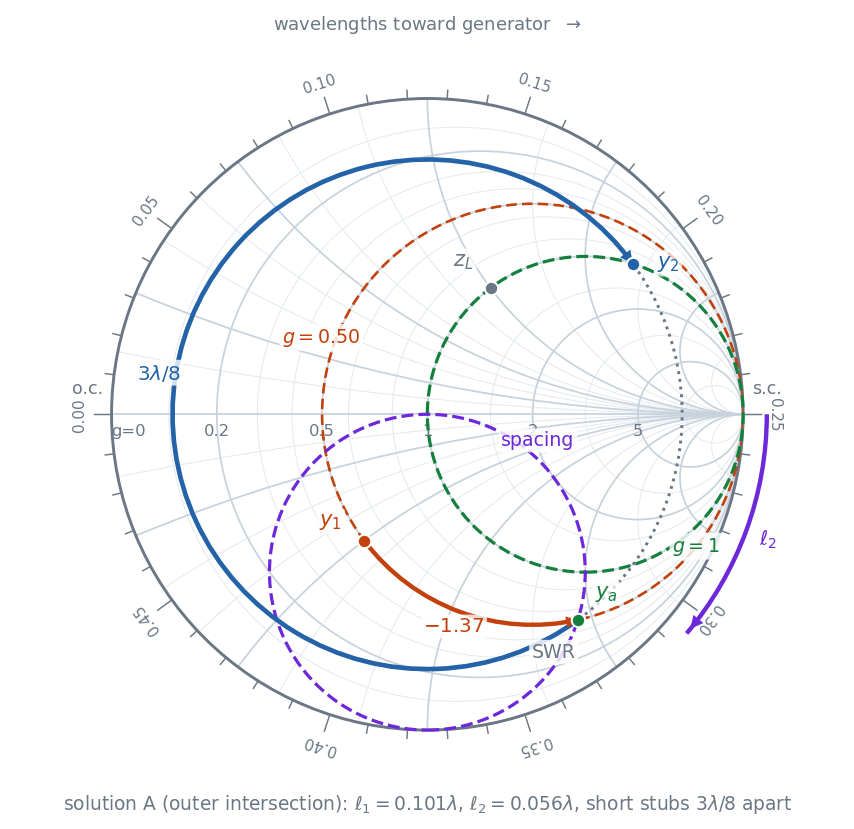
\includegraphics[width=0.495\textwidth]{figs/c2num_p08.png}\hfill
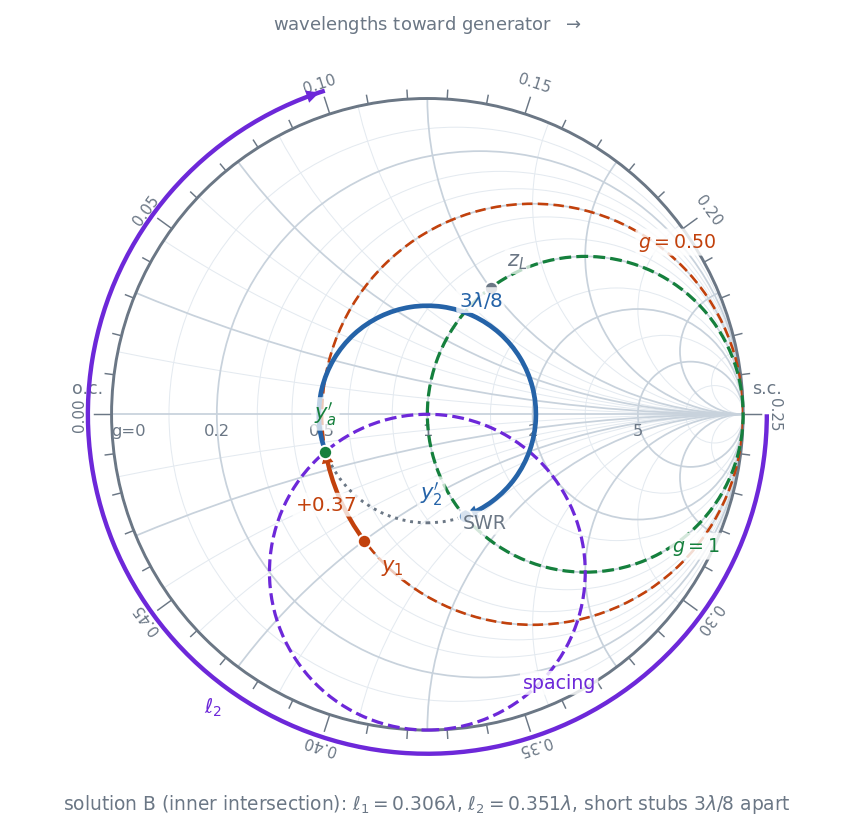
\includegraphics[width=0.495\textwidth]{figs/c2num_p08b.png}
\end{center}
{\footnotesize\color{sub} Problem 8 --- Smith chart construction, left: solution A, the outer intersection of the $g = 0.50$ circle with the spacing circle; right: solution B, the inner intersection of the $g = 0.50$ circle with the spacing circle.}

\figC{c2num_p08_line.png}{0.62\textwidth}
{\footnotesize\color{sub} Problem 8 --- line diagram of the matched network: shunt stubs across the line, lengths from the answer above.}

\figC{c2num_p08_coax.png}{0.69\textwidth}
{\footnotesize\color{sub} Problem 8 --- coaxial realisation, longitudinal section: each stub a coax tee off the main line; a shorting plate closes each stub.}

\penalty0\vspace{2pt}

%======================================================================
\Q{Problem 9 --- Double-stub shunt tuner}{\m{10}}
{\color{sub}\footnotesize \yr{\textbf{70 Bh}} \gap$\cdot$\gap $Z_0 = 100\,\Omega$}

\begin{asked}{\textbf{70 Bh} \ [10]}
Design a double-stub tuner ($3\lambda/8$ spacing) for $Z_L = 80+j180\,\Omega$ on a $100\,\Omega$ line at 3 GHz, with figure.
\end{asked}
\lead{Given}
\begin{itemize}
  \item $Z_L = 80.00 + j180.00\,\Omega$, $Z_0 = 100\,\Omega$.
  \item $f = 3\text{ GHz}$ $\Rightarrow$ $\lambda_0 = c/f = 99.9\text{ mm}$.
\end{itemize}
\lead{Step 1 --- normalise and plot $z_L$}
\begin{itemize}
  \item $z_L = Z_L/Z_0 = 80.00 + j180.00$ over $100$ $=0.80 + j1.80$.
  \item Plot it where the $r = 0.80$ circle cuts the $x = +1.80$ arc; it reads $0.179\lambda$ on the WTG scale.
  \item Dividers from centre to $z_L$ (the SWR-circle radius), laid on the radially scaled scales below the chart: $|\Gamma_L| = 0.711$ on \emph{refl.\ coeff.\ E or I}, $S = 5.93$ on \emph{SWR}. \textit{Check:} $(z_L-1)/(z_L+1) = 0.711\angle 51.3^\circ$, $(1+|\Gamma_L|)/(1-|\Gamma_L|) = 5.93$.
\end{itemize}
\lead{Step 2 --- convert to admittance}
\begin{itemize}
  \item Draw the diameter through $z_L$ and read the opposite intersection --- a $\lambda/4$ half-turn. On an immittance chart read the amber grid in place and skip this step.
  \item $y_L = 1/z_L = 0.21 - j0.46$, at $0.429\lambda$ on the WTG scale (exactly $0.25\lambda$ from $z_L$).
\end{itemize}
\lead{Step 3 --- the first stub is at the load}
\begin{itemize}
  \item No offset is specified, so stub 1 sits at the load and $y_1 = y_L = 0.21 - j0.46$.
\end{itemize}
\lead{Step 4 --- draw the spacing circle}
\begin{itemize}
  \item Rotate the $g=1$ circle $3\lambda/8$ \textbf{toward the load} (anticlockwise). Call the result the \textbf{spacing circle}.
  \item Any point on it is carried \emph{onto} $g=1$ by the $3\lambda/8$ of line between the two stubs --- which is exactly what stub 1 must aim for.
  \item Check the forbidden region first: matching needs $g_1 \le 1/\sin^2\beta d = 2.00$, and here $g_1 = 0.206$. \checkmark
\end{itemize}
\lead{Step 5 --- stub 1: slide along the constant-$g$ circle}
\begin{itemize}
  \item A shunt stub adds susceptance only, so the point can move \emph{only along its own $g = 0.206$ circle}.
  \item Follow that circle to where it cuts the spacing circle. It cuts twice, giving the two standard solutions (one chart each below):
  \begin{itemize}
    \item \textbf{Solution A} (outer intersection, nearer the rim): $y_a = 0.21 - j1.61$, so stub 1 must add $b_1 = -1.608 - (-0.464) = -1.144$.
    \item \textbf{Solution B} (inner intersection, nearer the centre): $y_a' = 0.21 - j0.39$, so $b_1' = +0.072$.
  \end{itemize}
  \item Read $\ell_1$ off the rim, starting at the short-circuit point ($y=\infty$, the right of the chart): $\ell_1 = 0.114\lambda$ (A) and $0.261\lambda$ (B).
\end{itemize}
\lead{Step 6 --- the $3\lambda/8$ of line between the stubs}
\begin{itemize}
  \item Swing a \emph{new} SWR circle through $y_a$ and rotate \textbf{clockwise} by $3\lambda/8$.
  \item By construction it lands on the $g=1$ circle: $y_2 = 1.00 + j3.95$ (A), $y_2' = 1.00 - j1.95$ (B).
\end{itemize}
\lead{Step 7 --- stub 2 cancels what is left}
\begin{itemize}
  \item Stub 2 supplies $b_2 = -3.950$ (A) or $+1.950$ (B), leaving $y_{in} = 1 + j0$, i.e. $Z_{in} = Z_0 = 100\,\Omega$. Matched.
  \item Off the rim from the short-circuit point ($y=\infty$, the right of the chart): $\ell_2 = 0.039\lambda$ (A) and $0.425\lambda$ (B).
\end{itemize}
\lead{Answer}
\begin{tabularx}{\linewidth}{@{}L{3.2cm}X X@{}}
\toprule
\hrow \thead{Quantity} & \thead{Solution A} & \thead{Solution B} \\
\midrule
Stub spacing $d$ & $3\lambda/8$ & $3\lambda/8$ \\
First stub from load & $0.000\lambda$ & $0.000\lambda$ \\
$y$ before stub 1 & $0.21 - j0.46$ & $0.21 - j0.46$ \\
Stub 1 susceptance $b_1$ & $-1.144$ & $+0.072$ \\
\textbf{Stub 1 length $\ell_1$} & $0.114\lambda$ & $0.261\lambda$ \\
$y$ after the spacing & $1.00 + j3.95$ & $1.00 - j1.95$ \\
Stub 2 susceptance $b_2$ & $-3.950$ & $+1.950$ \\
\textbf{Stub 2 length $\ell_2$} & $0.039\lambda$ & $0.425\lambda$ \\
\bottomrule
\end{tabularx}

\lead{Both are correct.} Quote either, but say which you chose. Solution A uses the shorter stubs here, which is the practical pick: less line at high VSWR means lower loss and wider bandwidth.

\begin{center}
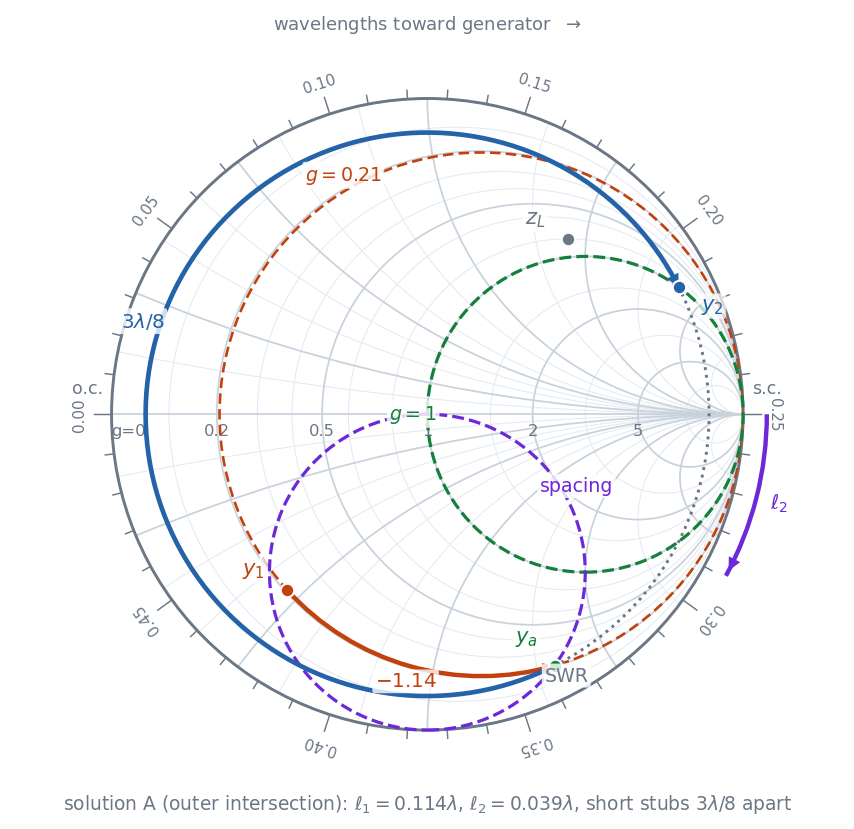
\includegraphics[width=0.495\textwidth]{figs/c2num_p09.png}\hfill
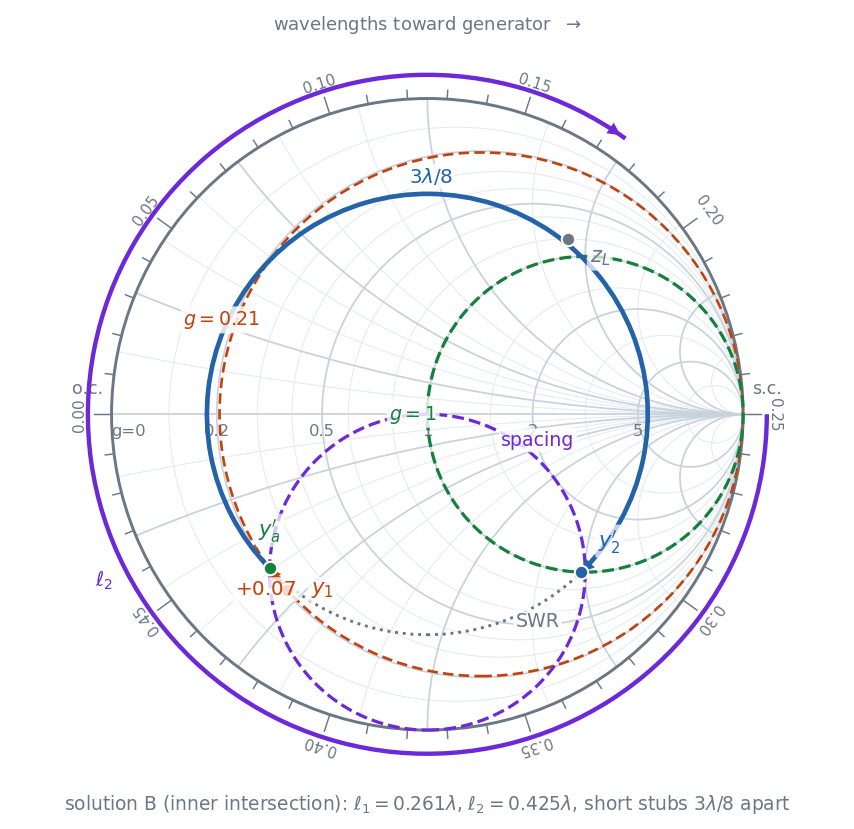
\includegraphics[width=0.495\textwidth]{figs/c2num_p09b.png}
\end{center}
{\footnotesize\color{sub} Problem 9 --- Smith chart construction, left: solution A, the outer intersection of the $g = 0.21$ circle with the spacing circle; right: solution B, the inner intersection of the $g = 0.21$ circle with the spacing circle.}

\figC{c2num_p09_line.png}{0.62\textwidth}
{\footnotesize\color{sub} Problem 9 --- line diagram of the matched network: shunt stubs across the line, lengths from the answer above.}

\figC{c2num_p09_coax.png}{0.69\textwidth}
{\footnotesize\color{sub} Problem 9 --- coaxial realisation, longitudinal section: each stub a coax tee off the main line; a shorting plate closes each stub.}

\penalty0\vspace{2pt}

%======================================================================
\Q{Problem 10 --- Double-stub shunt tuner}{\m{10}}
{\color{sub}\footnotesize \yr{70 Ma} \gap$\cdot$\gap $Z_0 = 100\,\Omega$}

\begin{asked}{70 Ma \ [10]}
Design a double-stub tuner ($3\lambda/8$ spacing) for $Z_L = 190+j110\,\Omega$ on a $100\,\Omega$ line at 10 GHz, with figure.
\end{asked}
\lead{Given}
\begin{itemize}
  \item $Z_L = 190.00 + j110.00\,\Omega$, $Z_0 = 100\,\Omega$.
  \item $f = 10\text{ GHz}$ $\Rightarrow$ $\lambda_0 = c/f = 30.0\text{ mm}$.
\end{itemize}
\lead{Step 1 --- normalise and plot $z_L$}
\begin{itemize}
  \item $z_L = Z_L/Z_0 = 190.00 + j110.00$ over $100$ $=1.90 + j1.10$.
  \item Plot it where the $r = 1.90$ circle cuts the $x = +1.10$ arc; it reads $0.208\lambda$ on the WTG scale.
  \item Dividers from centre to $z_L$ (the SWR-circle radius), laid on the radially scaled scales below the chart: $|\Gamma_L| = 0.458$ on \emph{refl.\ coeff.\ E or I}, $S = 2.69$ on \emph{SWR}. \textit{Check:} $(z_L-1)/(z_L+1) = 0.458\angle 29.9^\circ$, $(1+|\Gamma_L|)/(1-|\Gamma_L|) = 2.69$.
\end{itemize}
\lead{Step 2 --- convert to admittance}
\begin{itemize}
  \item Draw the diameter through $z_L$ and read the opposite intersection --- a $\lambda/4$ half-turn. On an immittance chart read the amber grid in place and skip this step.
  \item $y_L = 1/z_L = 0.39 - j0.23$, at $0.458\lambda$ on the WTG scale (exactly $0.25\lambda$ from $z_L$).
\end{itemize}
\lead{Step 3 --- the first stub is at the load}
\begin{itemize}
  \item No offset is specified, so stub 1 sits at the load and $y_1 = y_L = 0.39 - j0.23$.
\end{itemize}
\lead{Step 4 --- draw the spacing circle}
\begin{itemize}
  \item Rotate the $g=1$ circle $3\lambda/8$ \textbf{toward the load} (anticlockwise). Call the result the \textbf{spacing circle}.
  \item Any point on it is carried \emph{onto} $g=1$ by the $3\lambda/8$ of line between the two stubs --- which is exactly what stub 1 must aim for.
  \item Check the forbidden region first: matching needs $g_1 \le 1/\sin^2\beta d = 2.00$, and here $g_1 = 0.394$. \checkmark
\end{itemize}
\lead{Step 5 --- stub 1: slide along the constant-$g$ circle}
\begin{itemize}
  \item A shunt stub adds susceptance only, so the point can move \emph{only along its own $g = 0.394$ circle}.
  \item Follow that circle to where it cuts the spacing circle. It cuts twice, giving the two standard solutions (one chart each below):
  \begin{itemize}
    \item \textbf{Solution A} (outer intersection, nearer the rim): $y_a = 0.39 - j1.80$, so stub 1 must add $b_1 = -1.796 - (-0.228) = -1.567$.
    \item \textbf{Solution B} (inner intersection, nearer the centre): $y_a' = 0.39 - j0.20$, so $b_1' = +0.024$.
  \end{itemize}
  \item Read $\ell_1$ off the rim, starting at the short-circuit point ($y=\infty$, the right of the chart): $\ell_1 = 0.090\lambda$ (A) and $0.254\lambda$ (B).
\end{itemize}
\lead{Step 6 --- the $3\lambda/8$ of line between the stubs}
\begin{itemize}
  \item Swing a \emph{new} SWR circle through $y_a$ and rotate \textbf{clockwise} by $3\lambda/8$.
  \item By construction it lands on the $g=1$ circle: $y_2 = 1.00 + j3.02$ (A), $y_2' = 1.00 - j1.02$ (B).
\end{itemize}
\lead{Step 7 --- stub 2 cancels what is left}
\begin{itemize}
  \item Stub 2 supplies $b_2 = -3.018$ (A) or $+1.018$ (B), leaving $y_{in} = 1 + j0$, i.e. $Z_{in} = Z_0 = 100\,\Omega$. Matched.
  \item Off the rim from the short-circuit point ($y=\infty$, the right of the chart): $\ell_2 = 0.051\lambda$ (A) and $0.376\lambda$ (B).
\end{itemize}
\lead{Answer}
\begin{tabularx}{\linewidth}{@{}L{3.2cm}X X@{}}
\toprule
\hrow \thead{Quantity} & \thead{Solution A} & \thead{Solution B} \\
\midrule
Stub spacing $d$ & $3\lambda/8$ & $3\lambda/8$ \\
First stub from load & $0.000\lambda$ & $0.000\lambda$ \\
$y$ before stub 1 & $0.39 - j0.23$ & $0.39 - j0.23$ \\
Stub 1 susceptance $b_1$ & $-1.567$ & $+0.024$ \\
\textbf{Stub 1 length $\ell_1$} & $0.090\lambda$ & $0.254\lambda$ \\
$y$ after the spacing & $1.00 + j3.02$ & $1.00 - j1.02$ \\
Stub 2 susceptance $b_2$ & $-3.018$ & $+1.018$ \\
\textbf{Stub 2 length $\ell_2$} & $0.051\lambda$ & $0.376\lambda$ \\
\bottomrule
\end{tabularx}

\lead{Both are correct.} Quote either, but say which you chose. Solution A uses the shorter stubs here, which is the practical pick: less line at high VSWR means lower loss and wider bandwidth.

\begin{center}
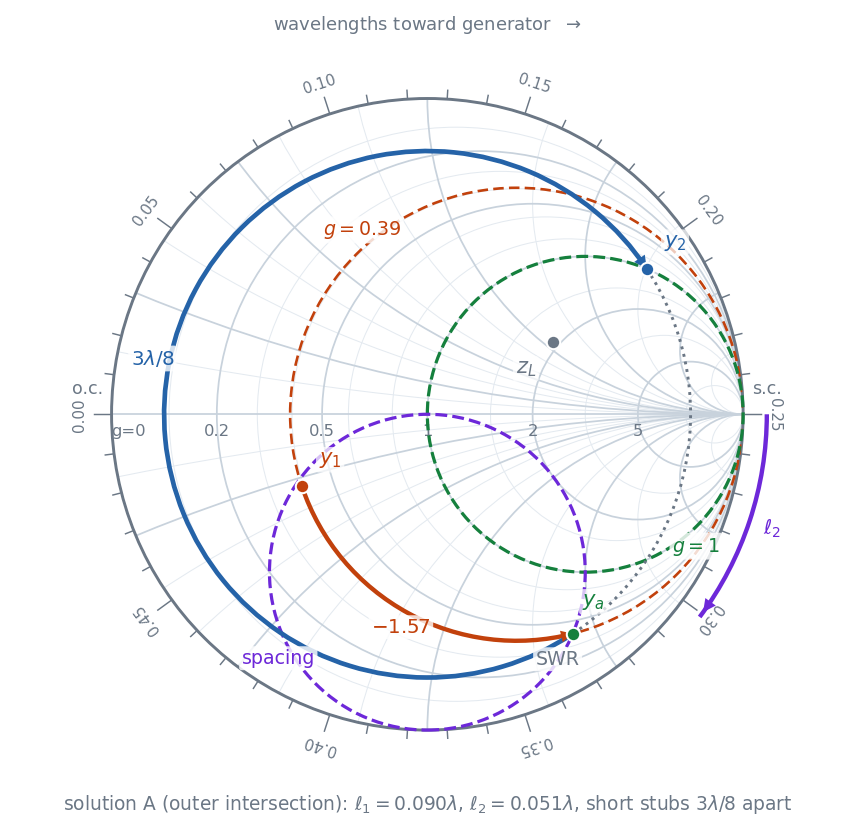
\includegraphics[width=0.495\textwidth]{figs/c2num_p10.png}\hfill
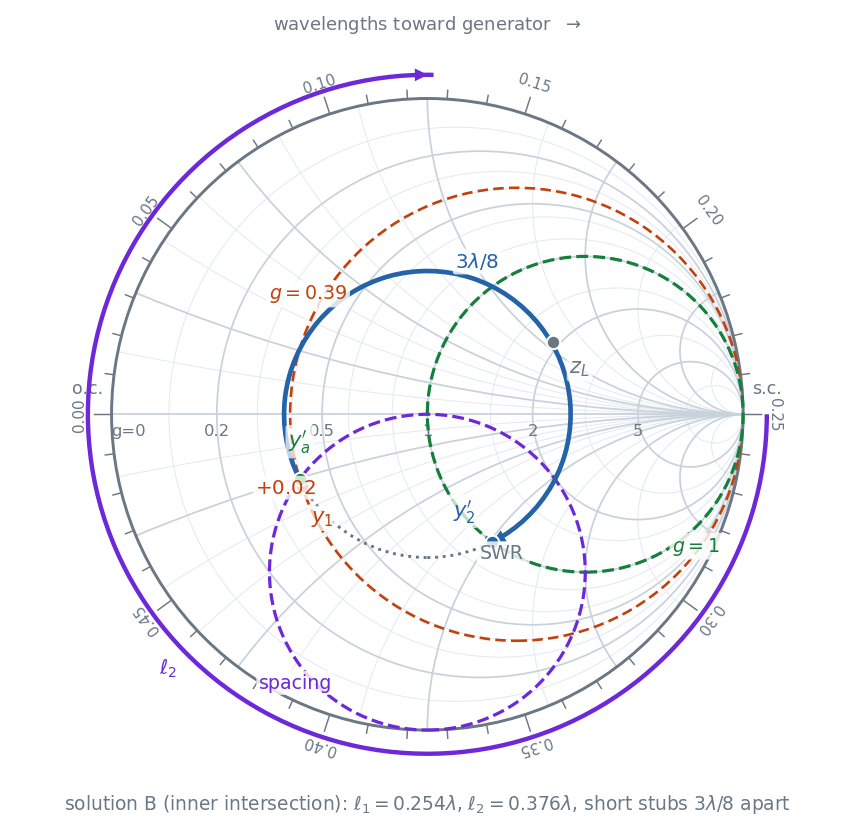
\includegraphics[width=0.495\textwidth]{figs/c2num_p10b.png}
\end{center}
{\footnotesize\color{sub} Problem 10 --- Smith chart construction, left: solution A, the outer intersection of the $g = 0.39$ circle with the spacing circle; right: solution B, the inner intersection of the $g = 0.39$ circle with the spacing circle.}

\figC{c2num_p10_line.png}{0.62\textwidth}
{\footnotesize\color{sub} Problem 10 --- line diagram of the matched network: shunt stubs across the line, lengths from the answer above.}

\figC{c2num_p10_coax.png}{0.69\textwidth}
{\footnotesize\color{sub} Problem 10 --- coaxial realisation, longitudinal section: each stub a coax tee off the main line; a shorting plate closes each stub.}

\penalty0\vspace{2pt}

%======================================================================
\Q{Problem 11 --- Double-stub shunt tuner}{\m{8}}
{\color{sub}\footnotesize \yr{73 Ma} \gap$\cdot$\gap $Z_0 = 50\,\Omega$}

\begin{asked}{73 Ma \ [8]}
Design a double-stub tuner for an inductive load on a $50\,\Omega$ line. Include the figure.
\end{asked}
\lead{Given}
\begin{itemize}
  \item $Z_L = 40.00 + j70.00\,\Omega$, $Z_0 = 50\,\Omega$.
  \item \added{} The paper leaves the values to the candidate; $Z_L = 40.00 + j70.00\,\Omega$ on a $50\,\Omega$ line is assumed here. Any complex load works --- the method is what earns the marks.
\end{itemize}
\lead{Step 1 --- normalise and plot $z_L$}
\begin{itemize}
  \item $z_L = Z_L/Z_0 = 40.00 + j70.00$ over $50$ $=0.80 + j1.40$.
  \item Plot it where the $r = 0.80$ circle cuts the $x = +1.40$ arc; it reads $0.166\lambda$ on the WTG scale.
  \item Dividers from centre to $z_L$ (the SWR-circle radius), laid on the radially scaled scales below the chart: $|\Gamma_L| = 0.620$ on \emph{refl.\ coeff.\ E or I}, $S = 4.27$ on \emph{SWR}. \textit{Check:} $(z_L-1)/(z_L+1) = 0.620\angle 60.3^\circ$, $(1+|\Gamma_L|)/(1-|\Gamma_L|) = 4.27$.
\end{itemize}
\lead{Step 2 --- convert to admittance}
\begin{itemize}
  \item Draw the diameter through $z_L$ and read the opposite intersection --- a $\lambda/4$ half-turn. On an immittance chart read the amber grid in place and skip this step.
  \item $y_L = 1/z_L = 0.31 - j0.54$, at $0.416\lambda$ on the WTG scale (exactly $0.25\lambda$ from $z_L$).
\end{itemize}
\lead{Step 3 --- the first stub is at the load}
\begin{itemize}
  \item No offset is specified, so stub 1 sits at the load and $y_1 = y_L = 0.31 - j0.54$.
\end{itemize}
\lead{Step 4 --- draw the spacing circle}
\begin{itemize}
  \item Rotate the $g=1$ circle $3\lambda/8$ \textbf{toward the load} (anticlockwise). Call the result the \textbf{spacing circle}.
  \item Any point on it is carried \emph{onto} $g=1$ by the $3\lambda/8$ of line between the two stubs --- which is exactly what stub 1 must aim for.
  \item Check the forbidden region first: matching needs $g_1 \le 1/\sin^2\beta d = 2.00$, and here $g_1 = 0.308$. \checkmark
\end{itemize}
\lead{Step 5 --- stub 1: slide along the constant-$g$ circle}
\begin{itemize}
  \item A shunt stub adds susceptance only, so the point can move \emph{only along its own $g = 0.308$ circle}.
  \item Follow that circle to where it cuts the spacing circle. It cuts twice, giving the two standard solutions (one chart each below):
  \begin{itemize}
    \item \textbf{Solution A} (outer intersection, nearer the rim): $y_a = 0.31 - j1.72$, so stub 1 must add $b_1 = -1.722 - (-0.538) = -1.183$.
    \item \textbf{Solution B} (inner intersection, nearer the centre): $y_a' = 0.31 - j0.28$, so $b_1' = +0.260$.
  \end{itemize}
  \item Read $\ell_1$ off the rim, starting at the short-circuit point ($y=\infty$, the right of the chart): $\ell_1 = 0.112\lambda$ (A) and $0.290\lambda$ (B).
\end{itemize}
\lead{Step 6 --- the $3\lambda/8$ of line between the stubs}
\begin{itemize}
  \item Swing a \emph{new} SWR circle through $y_a$ and rotate \textbf{clockwise} by $3\lambda/8$.
  \item By construction it lands on the $g=1$ circle: $y_2 = 1.00 + j3.35$ (A), $y_2' = 1.00 - j1.35$ (B).
\end{itemize}
\lead{Step 7 --- stub 2 cancels what is left}
\begin{itemize}
  \item Stub 2 supplies $b_2 = -3.345$ (A) or $+1.345$ (B), leaving $y_{in} = 1 + j0$, i.e. $Z_{in} = Z_0 = 50\,\Omega$. Matched.
  \item Off the rim from the short-circuit point ($y=\infty$, the right of the chart): $\ell_2 = 0.046\lambda$ (A) and $0.398\lambda$ (B).
\end{itemize}
\lead{Answer}
\begin{tabularx}{\linewidth}{@{}L{3.2cm}X X@{}}
\toprule
\hrow \thead{Quantity} & \thead{Solution A} & \thead{Solution B} \\
\midrule
Stub spacing $d$ & $3\lambda/8$ & $3\lambda/8$ \\
First stub from load & $0.000\lambda$ & $0.000\lambda$ \\
$y$ before stub 1 & $0.31 - j0.54$ & $0.31 - j0.54$ \\
Stub 1 susceptance $b_1$ & $-1.183$ & $+0.260$ \\
\textbf{Stub 1 length $\ell_1$} & $0.112\lambda$ & $0.290\lambda$ \\
$y$ after the spacing & $1.00 + j3.35$ & $1.00 - j1.35$ \\
Stub 2 susceptance $b_2$ & $-3.345$ & $+1.345$ \\
\textbf{Stub 2 length $\ell_2$} & $0.046\lambda$ & $0.398\lambda$ \\
\bottomrule
\end{tabularx}

\lead{Both are correct.} Quote either, but say which you chose. Solution A uses the shorter stubs here, which is the practical pick: less line at high VSWR means lower loss and wider bandwidth.

\begin{center}
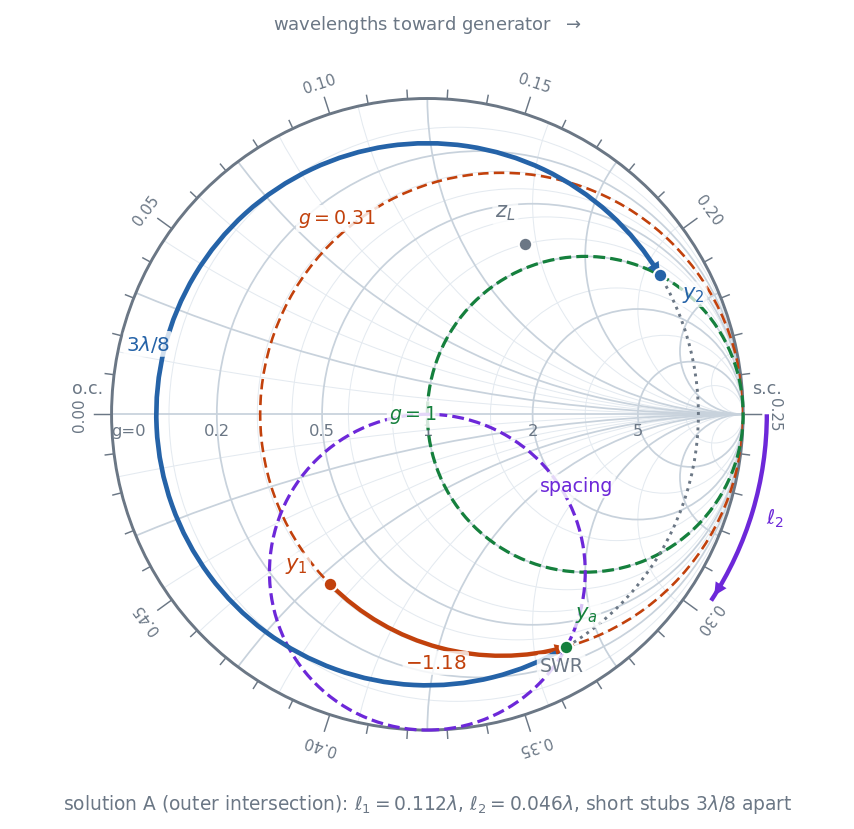
\includegraphics[width=0.495\textwidth]{figs/c2num_p11.png}\hfill
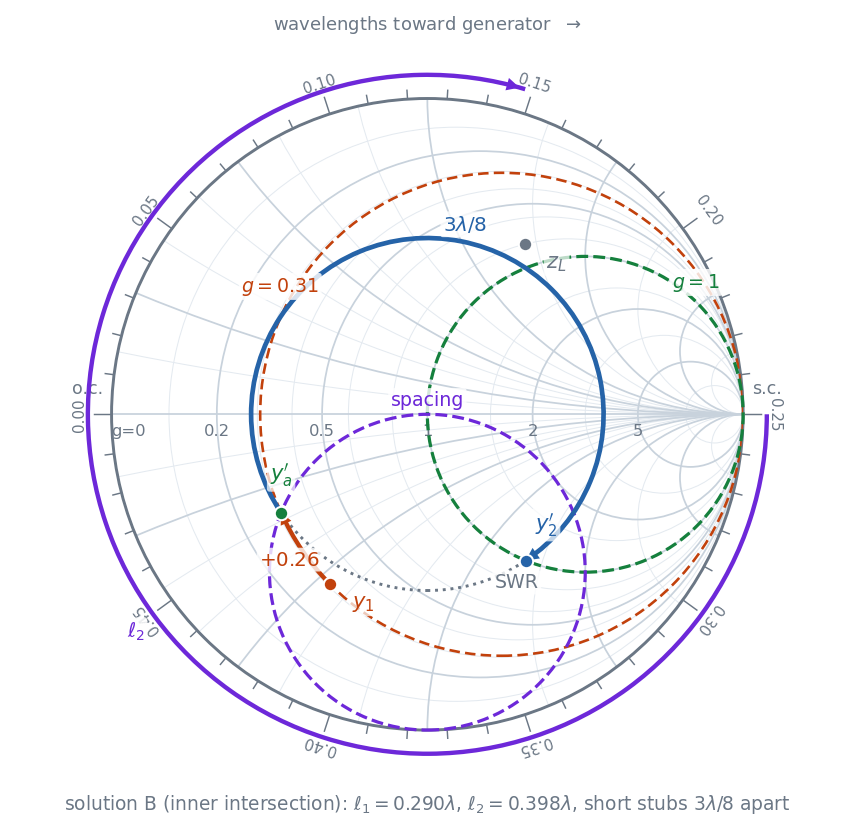
\includegraphics[width=0.495\textwidth]{figs/c2num_p11b.png}
\end{center}
{\footnotesize\color{sub} Problem 11 --- Smith chart construction, left: solution A, the outer intersection of the $g = 0.31$ circle with the spacing circle; right: solution B, the inner intersection of the $g = 0.31$ circle with the spacing circle.}

\figC{c2num_p11_line.png}{0.62\textwidth}
{\footnotesize\color{sub} Problem 11 --- line diagram of the matched network: shunt stubs across the line, lengths from the answer above.}

\figC{c2num_p11_coax.png}{0.69\textwidth}
{\footnotesize\color{sub} Problem 11 --- coaxial realisation, longitudinal section: each stub a coax tee off the main line; a shorting plate closes each stub.}

\penalty0\vspace{2pt}

%======================================================================
\Q{Problem 12 --- Double-stub shunt tuner}{\m{3}\m{15}}
{\color{sub}\footnotesize \yr{\textbf{69 Bh}} \gap$\cdot$\gap $Z_0 = 50\,\Omega$}

\begin{asked}{\textbf{69 Bh} \ [3+15]}
Design a short-circuited double-stub tuner with $3\lambda/8$ spacing for $Z_L = 75+j75\,\Omega$ on a $50\,\Omega$ line.
\end{asked}
\lead{Given}
\begin{itemize}
  \item $Z_L = 75.00 + j75.00\,\Omega$, $Z_0 = 50\,\Omega$.
\end{itemize}
\lead{Step 1 --- normalise and plot $z_L$}
\begin{itemize}
  \item $z_L = Z_L/Z_0 = 75.00 + j75.00$ over $50$ $=1.50 + j1.50$.
  \item Plot it where the $r = 1.50$ circle cuts the $x = +1.50$ arc; it reads $0.194\lambda$ on the WTG scale.
  \item Dividers from centre to $z_L$ (the SWR-circle radius), laid on the radially scaled scales below the chart: $|\Gamma_L| = 0.542$ on \emph{refl.\ coeff.\ E or I}, $S = 3.37$ on \emph{SWR}. \textit{Check:} $(z_L-1)/(z_L+1) = 0.542\angle 40.6^\circ$, $(1+|\Gamma_L|)/(1-|\Gamma_L|) = 3.37$.
\end{itemize}
\lead{Step 2 --- convert to admittance}
\begin{itemize}
  \item Draw the diameter through $z_L$ and read the opposite intersection --- a $\lambda/4$ half-turn. On an immittance chart read the amber grid in place and skip this step.
  \item $y_L = 1/z_L = 0.33 - j0.33$, at $0.444\lambda$ on the WTG scale (exactly $0.25\lambda$ from $z_L$).
\end{itemize}
\lead{Step 3 --- the first stub is at the load}
\begin{itemize}
  \item No offset is specified, so stub 1 sits at the load and $y_1 = y_L = 0.33 - j0.33$.
\end{itemize}
\lead{Step 4 --- draw the spacing circle}
\begin{itemize}
  \item Rotate the $g=1$ circle $3\lambda/8$ \textbf{toward the load} (anticlockwise). Call the result the \textbf{spacing circle}.
  \item Any point on it is carried \emph{onto} $g=1$ by the $3\lambda/8$ of line between the two stubs --- which is exactly what stub 1 must aim for.
  \item Check the forbidden region first: matching needs $g_1 \le 1/\sin^2\beta d = 2.00$, and here $g_1 = 0.333$. \checkmark
\end{itemize}
\lead{Step 5 --- stub 1: slide along the constant-$g$ circle}
\begin{itemize}
  \item A shunt stub adds susceptance only, so the point can move \emph{only along its own $g = 0.333$ circle}.
  \item Follow that circle to where it cuts the spacing circle. It cuts twice, giving the two standard solutions (one chart each below):
  \begin{itemize}
    \item \textbf{Solution A} (outer intersection, nearer the rim): $y_a = 0.33 - j1.75$, so stub 1 must add $b_1 = -1.745 - (-0.333) = -1.412$.
    \item \textbf{Solution B} (inner intersection, nearer the centre): $y_a' = 0.33 - j0.25$, so $b_1' = +0.079$.
  \end{itemize}
  \item Read $\ell_1$ off the rim, starting at the short-circuit point ($y=\infty$, the right of the chart): $\ell_1 = 0.098\lambda$ (A) and $0.262\lambda$ (B).
\end{itemize}
\lead{Step 6 --- the $3\lambda/8$ of line between the stubs}
\begin{itemize}
  \item Swing a \emph{new} SWR circle through $y_a$ and rotate \textbf{clockwise} by $3\lambda/8$.
  \item By construction it lands on the $g=1$ circle: $y_2 = 1.00 + j3.24$ (A), $y_2' = 1.00 - j1.24$ (B).
\end{itemize}
\lead{Step 7 --- stub 2 cancels what is left}
\begin{itemize}
  \item Stub 2 supplies $b_2 = -3.236$ (A) or $+1.236$ (B), leaving $y_{in} = 1 + j0$, i.e. $Z_{in} = Z_0 = 50\,\Omega$. Matched.
  \item Off the rim from the short-circuit point ($y=\infty$, the right of the chart): $\ell_2 = 0.048\lambda$ (A) and $0.392\lambda$ (B).
\end{itemize}
\lead{Answer}
\begin{tabularx}{\linewidth}{@{}L{3.2cm}X X@{}}
\toprule
\hrow \thead{Quantity} & \thead{Solution A} & \thead{Solution B} \\
\midrule
Stub spacing $d$ & $3\lambda/8$ & $3\lambda/8$ \\
First stub from load & $0.000\lambda$ & $0.000\lambda$ \\
$y$ before stub 1 & $0.33 - j0.33$ & $0.33 - j0.33$ \\
Stub 1 susceptance $b_1$ & $-1.412$ & $+0.079$ \\
\textbf{Stub 1 length $\ell_1$} & $0.098\lambda$ & $0.262\lambda$ \\
$y$ after the spacing & $1.00 + j3.24$ & $1.00 - j1.24$ \\
Stub 2 susceptance $b_2$ & $-3.236$ & $+1.236$ \\
\textbf{Stub 2 length $\ell_2$} & $0.048\lambda$ & $0.392\lambda$ \\
\bottomrule
\end{tabularx}

\lead{Both are correct.} Quote either, but say which you chose. Solution A uses the shorter stubs here, which is the practical pick: less line at high VSWR means lower loss and wider bandwidth.

\begin{center}
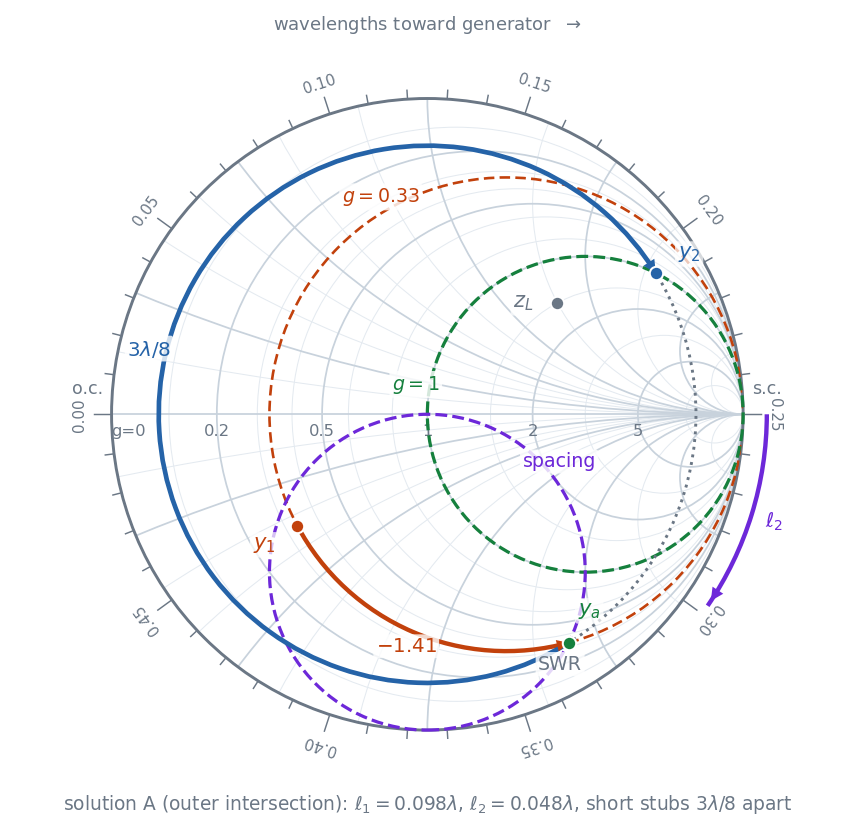
\includegraphics[width=0.495\textwidth]{figs/c2num_p12.png}\hfill
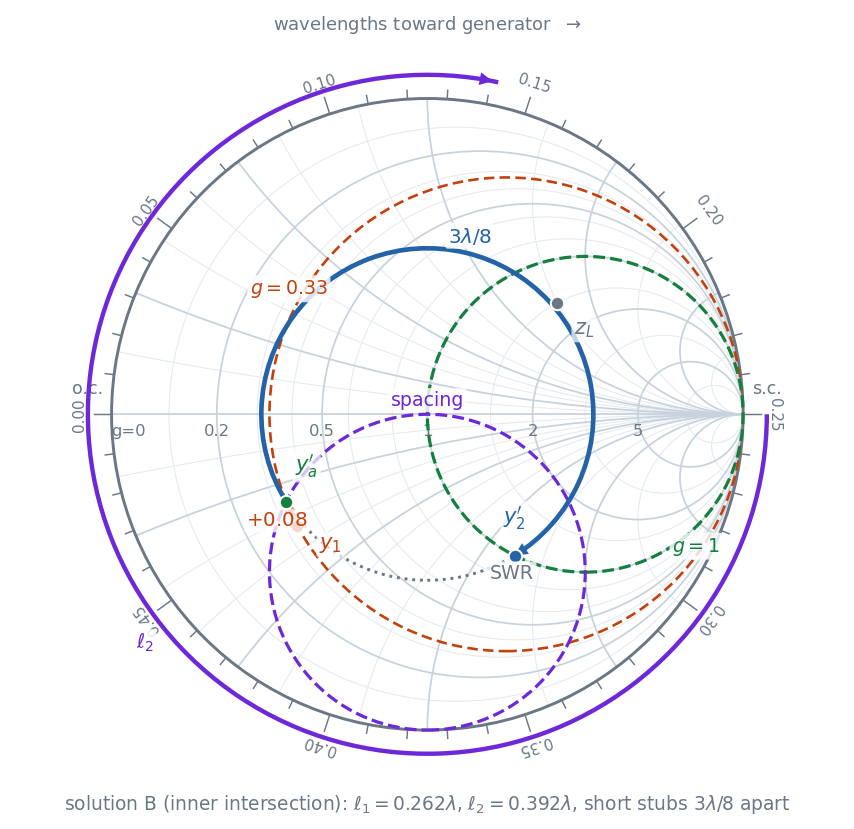
\includegraphics[width=0.495\textwidth]{figs/c2num_p12b.png}
\end{center}
{\footnotesize\color{sub} Problem 12 --- Smith chart construction, left: solution A, the outer intersection of the $g = 0.33$ circle with the spacing circle; right: solution B, the inner intersection of the $g = 0.33$ circle with the spacing circle.}

\figC{c2num_p12_line.png}{0.62\textwidth}
{\footnotesize\color{sub} Problem 12 --- line diagram of the matched network: shunt stubs across the line, lengths from the answer above.}

\figC{c2num_p12_coax.png}{0.69\textwidth}
{\footnotesize\color{sub} Problem 12 --- coaxial realisation, longitudinal section: each stub a coax tee off the main line; a shorting plate closes each stub.}

\penalty0\vspace{2pt}

%======================================================================
\Q{Problem 13 --- Double-stub shunt tuner}{\m{8}\m{2}}
{\color{sub}\footnotesize \yr{\textbf{73 Bh}} \gap$\cdot$\gap $Z_0 = 78\,\Omega$}

\begin{asked}{\textbf{73 Bh} \ [8+2]}
Design a short-circuited double-stub tuner for a complex inductive load on a $78.0\,\Omega$ line, with figure.
\end{asked}
\lead{Given}
\begin{itemize}
  \item $Z_L = 95.00 + j85.00\,\Omega$, $Z_0 = 78\,\Omega$.
  \item \added{} The paper leaves the values to the candidate; $Z_L = 95.00 + j85.00\,\Omega$ on a $78\,\Omega$ line is assumed here. Any complex load works --- the method is what earns the marks.
\end{itemize}
\lead{Step 1 --- normalise and plot $z_L$}
\begin{itemize}
  \item $z_L = Z_L/Z_0 = 95.00 + j85.00$ over $78$ $=1.22 + j1.09$.
  \item Plot it where the $r = 1.22$ circle cuts the $x = +1.09$ arc; it reads $0.177\lambda$ on the WTG scale.
  \item Dividers from centre to $z_L$ (the SWR-circle radius), laid on the radially scaled scales below the chart: $|\Gamma_L| = 0.450$ on \emph{refl.\ coeff.\ E or I}, $S = 2.63$ on \emph{SWR}. \textit{Check:} $(z_L-1)/(z_L+1) = 0.450\angle 52.5^\circ$, $(1+|\Gamma_L|)/(1-|\Gamma_L|) = 2.63$.
\end{itemize}
\lead{Step 2 --- convert to admittance}
\begin{itemize}
  \item Draw the diameter through $z_L$ and read the opposite intersection --- a $\lambda/4$ half-turn. On an immittance chart read the amber grid in place and skip this step.
  \item $y_L = 1/z_L = 0.46 - j0.41$, at $0.427\lambda$ on the WTG scale (exactly $0.25\lambda$ from $z_L$).
\end{itemize}
\lead{Step 3 --- the first stub is at the load}
\begin{itemize}
  \item No offset is specified, so stub 1 sits at the load and $y_1 = y_L = 0.46 - j0.41$.
\end{itemize}
\lead{Step 4 --- draw the spacing circle}
\begin{itemize}
  \item Rotate the $g=1$ circle $3\lambda/8$ \textbf{toward the load} (anticlockwise). Call the result the \textbf{spacing circle}.
  \item Any point on it is carried \emph{onto} $g=1$ by the $3\lambda/8$ of line between the two stubs --- which is exactly what stub 1 must aim for.
  \item Check the forbidden region first: matching needs $g_1 \le 1/\sin^2\beta d = 2.00$, and here $g_1 = 0.456$. \checkmark
\end{itemize}
\lead{Step 5 --- stub 1: slide along the constant-$g$ circle}
\begin{itemize}
  \item A shunt stub adds susceptance only, so the point can move \emph{only along its own $g = 0.456$ circle}.
  \item Follow that circle to where it cuts the spacing circle. It cuts twice, giving the two standard solutions (one chart each below):
  \begin{itemize}
    \item \textbf{Solution A} (outer intersection, nearer the rim): $y_a = 0.46 - j1.84$, so stub 1 must add $b_1 = -1.839 - (-0.408) = -1.431$.
    \item \textbf{Solution B} (inner intersection, nearer the centre): $y_a' = 0.46 - j0.16$, so $b_1' = +0.247$.
  \end{itemize}
  \item Read $\ell_1$ off the rim, starting at the short-circuit point ($y=\infty$, the right of the chart): $\ell_1 = 0.097\lambda$ (A) and $0.289\lambda$ (B).
\end{itemize}
\lead{Step 6 --- the $3\lambda/8$ of line between the stubs}
\begin{itemize}
  \item Swing a \emph{new} SWR circle through $y_a$ and rotate \textbf{clockwise} by $3\lambda/8$.
  \item By construction it lands on the $g=1$ circle: $y_2 = 1.00 + j2.84$ (A), $y_2' = 1.00 - j0.84$ (B).
\end{itemize}
\lead{Step 7 --- stub 2 cancels what is left}
\begin{itemize}
  \item Stub 2 supplies $b_2 = -2.840$ (A) or $+0.840$ (B), leaving $y_{in} = 1 + j0$, i.e. $Z_{in} = Z_0 = 78\,\Omega$. Matched.
  \item Off the rim from the short-circuit point ($y=\infty$, the right of the chart): $\ell_2 = 0.054\lambda$ (A) and $0.361\lambda$ (B).
\end{itemize}
\lead{Answer}
\begin{tabularx}{\linewidth}{@{}L{3.2cm}X X@{}}
\toprule
\hrow \thead{Quantity} & \thead{Solution A} & \thead{Solution B} \\
\midrule
Stub spacing $d$ & $3\lambda/8$ & $3\lambda/8$ \\
First stub from load & $0.000\lambda$ & $0.000\lambda$ \\
$y$ before stub 1 & $0.46 - j0.41$ & $0.46 - j0.41$ \\
Stub 1 susceptance $b_1$ & $-1.431$ & $+0.247$ \\
\textbf{Stub 1 length $\ell_1$} & $0.097\lambda$ & $0.289\lambda$ \\
$y$ after the spacing & $1.00 + j2.84$ & $1.00 - j0.84$ \\
Stub 2 susceptance $b_2$ & $-2.840$ & $+0.840$ \\
\textbf{Stub 2 length $\ell_2$} & $0.054\lambda$ & $0.361\lambda$ \\
\bottomrule
\end{tabularx}

\lead{Both are correct.} Quote either, but say which you chose. Solution A uses the shorter stubs here, which is the practical pick: less line at high VSWR means lower loss and wider bandwidth.

\begin{center}
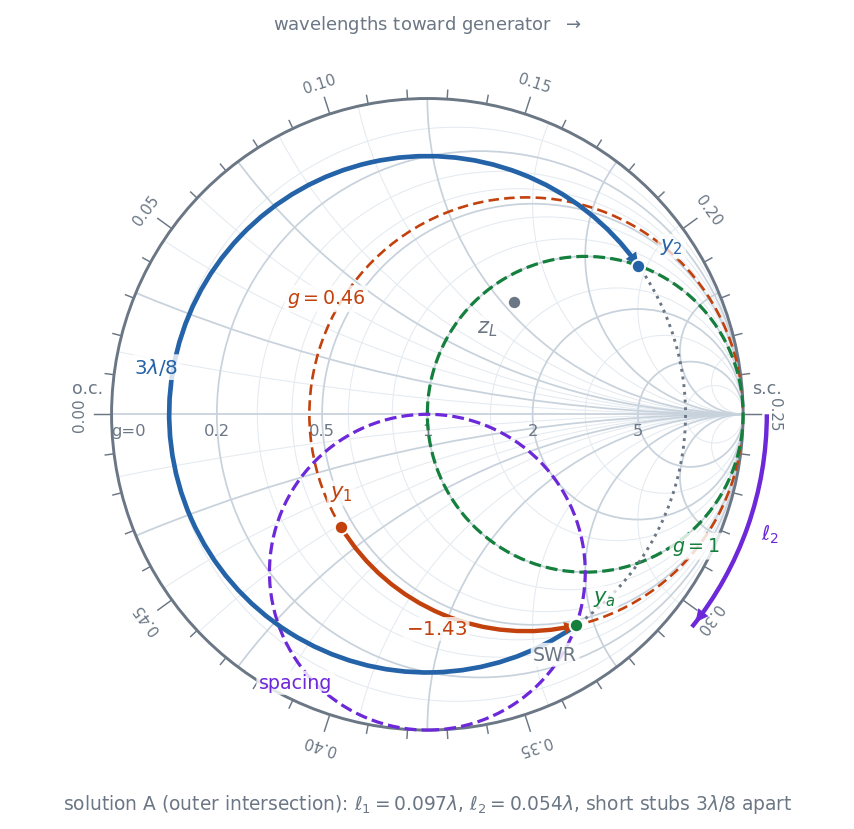
\includegraphics[width=0.495\textwidth]{figs/c2num_p13.png}\hfill
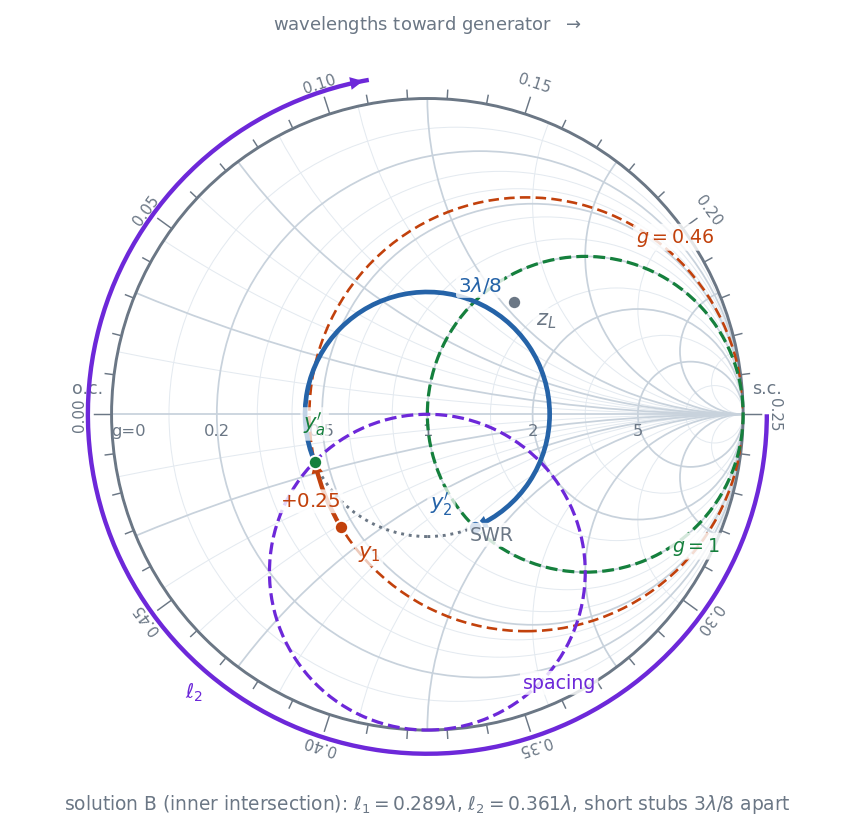
\includegraphics[width=0.495\textwidth]{figs/c2num_p13b.png}
\end{center}
{\footnotesize\color{sub} Problem 13 --- Smith chart construction, left: solution A, the outer intersection of the $g = 0.46$ circle with the spacing circle; right: solution B, the inner intersection of the $g = 0.46$ circle with the spacing circle.}

\figC{c2num_p13_line.png}{0.62\textwidth}
{\footnotesize\color{sub} Problem 13 --- line diagram of the matched network: shunt stubs across the line, lengths from the answer above.}

\figC{c2num_p13_coax.png}{0.69\textwidth}
{\footnotesize\color{sub} Problem 13 --- coaxial realisation, longitudinal section: each stub a coax tee off the main line; a shorting plate closes each stub.}

\penalty0\vspace{2pt}

%======================================================================
\Q{Problem 14 --- Double-stub shunt tuner}{\m{10}\m{2}}
{\color{sub}\footnotesize \yr{\textbf{75 Bh}} \gap$\cdot$\gap $Z_0 = 75\,\Omega$}

\begin{asked}{\textbf{75 Bh} \ [10+2]}
A $75\,\Omega$ coaxial line feeds a load of normalised impedance $z_L = 0.4+j0.85$. Design a short-circuited double-stub tuner.
\end{asked}
\lead{Given}
\begin{itemize}
  \item $Z_L = 30.00 + j63.75\,\Omega$, $Z_0 = 75\,\Omega$.
\end{itemize}
\lead{Step 1 --- normalise and plot $z_L$}
\begin{itemize}
  \item $z_L = Z_L/Z_0 = 30.00 + j63.75$ over $75$ $=0.40 + j0.85$.
  \item Plot it where the $r = 0.40$ circle cuts the $x = +0.85$ arc; it reads $0.120\lambda$ on the WTG scale.
  \item Dividers from centre to $z_L$ (the SWR-circle radius), laid on the radially scaled scales below the chart: $|\Gamma_L| = 0.635$ on \emph{refl.\ coeff.\ E or I}, $S = 4.48$ on \emph{SWR}. \textit{Check:} $(z_L-1)/(z_L+1) = 0.635\angle 94.0^\circ$, $(1+|\Gamma_L|)/(1-|\Gamma_L|) = 4.48$.
\end{itemize}
\lead{Step 2 --- convert to admittance}
\begin{itemize}
  \item Draw the diameter through $z_L$ and read the opposite intersection --- a $\lambda/4$ half-turn. On an immittance chart read the amber grid in place and skip this step.
  \item $y_L = 1/z_L = 0.45 - j0.96$, at $0.370\lambda$ on the WTG scale (exactly $0.25\lambda$ from $z_L$).
\end{itemize}
\lead{Step 3 --- the first stub is at the load}
\begin{itemize}
  \item No offset is specified, so stub 1 sits at the load and $y_1 = y_L = 0.45 - j0.96$.
\end{itemize}
\lead{Step 4 --- draw the spacing circle}
\begin{itemize}
  \item Rotate the $g=1$ circle $3\lambda/8$ \textbf{toward the load} (anticlockwise). Call the result the \textbf{spacing circle}.
  \item Any point on it is carried \emph{onto} $g=1$ by the $3\lambda/8$ of line between the two stubs --- which is exactly what stub 1 must aim for.
  \item Check the forbidden region first: matching needs $g_1 \le 1/\sin^2\beta d = 2.00$, and here $g_1 = 0.453$. \checkmark
\end{itemize}
\lead{Step 5 --- stub 1: slide along the constant-$g$ circle}
\begin{itemize}
  \item A shunt stub adds susceptance only, so the point can move \emph{only along its own $g = 0.453$ circle}.
  \item Follow that circle to where it cuts the spacing circle. It cuts twice, giving the two standard solutions (one chart each below):
  \begin{itemize}
    \item \textbf{Solution A} (outer intersection, nearer the rim): $y_a = 0.45 - j1.84$, so stub 1 must add $b_1 = -1.837 - (-0.963) = -0.874$.
    \item \textbf{Solution B} (inner intersection, nearer the centre): $y_a' = 0.45 - j0.16$, so $b_1' = +0.800$.
  \end{itemize}
  \item Read $\ell_1$ off the rim, starting at the short-circuit point ($y=\infty$, the right of the chart): $\ell_1 = 0.136\lambda$ (A) and $0.357\lambda$ (B).
\end{itemize}
\lead{Step 6 --- the $3\lambda/8$ of line between the stubs}
\begin{itemize}
  \item Swing a \emph{new} SWR circle through $y_a$ and rotate \textbf{clockwise} by $3\lambda/8$.
  \item By construction it lands on the $g=1$ circle: $y_2 = 1.00 + j2.85$ (A), $y_2' = 1.00 - j0.85$ (B).
\end{itemize}
\lead{Step 7 --- stub 2 cancels what is left}
\begin{itemize}
  \item Stub 2 supplies $b_2 = -2.847$ (A) or $+0.847$ (B), leaving $y_{in} = 1 + j0$, i.e. $Z_{in} = Z_0 = 75\,\Omega$. Matched.
  \item Off the rim from the short-circuit point ($y=\infty$, the right of the chart): $\ell_2 = 0.054\lambda$ (A) and $0.362\lambda$ (B).
\end{itemize}
\lead{Answer}
\begin{tabularx}{\linewidth}{@{}L{3.2cm}X X@{}}
\toprule
\hrow \thead{Quantity} & \thead{Solution A} & \thead{Solution B} \\
\midrule
Stub spacing $d$ & $3\lambda/8$ & $3\lambda/8$ \\
First stub from load & $0.000\lambda$ & $0.000\lambda$ \\
$y$ before stub 1 & $0.45 - j0.96$ & $0.45 - j0.96$ \\
Stub 1 susceptance $b_1$ & $-0.874$ & $+0.800$ \\
\textbf{Stub 1 length $\ell_1$} & $0.136\lambda$ & $0.357\lambda$ \\
$y$ after the spacing & $1.00 + j2.85$ & $1.00 - j0.85$ \\
Stub 2 susceptance $b_2$ & $-2.847$ & $+0.847$ \\
\textbf{Stub 2 length $\ell_2$} & $0.054\lambda$ & $0.362\lambda$ \\
\bottomrule
\end{tabularx}

\lead{Both are correct.} Quote either, but say which you chose. Solution A uses the shorter stubs here, which is the practical pick: less line at high VSWR means lower loss and wider bandwidth.

\begin{center}
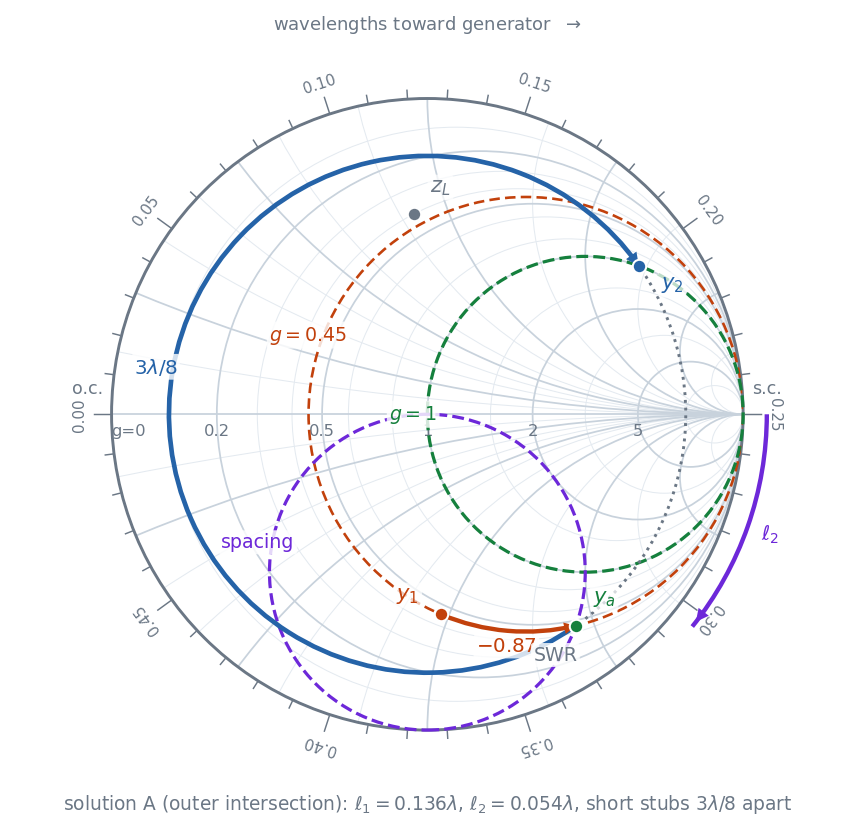
\includegraphics[width=0.495\textwidth]{figs/c2num_p14.png}\hfill
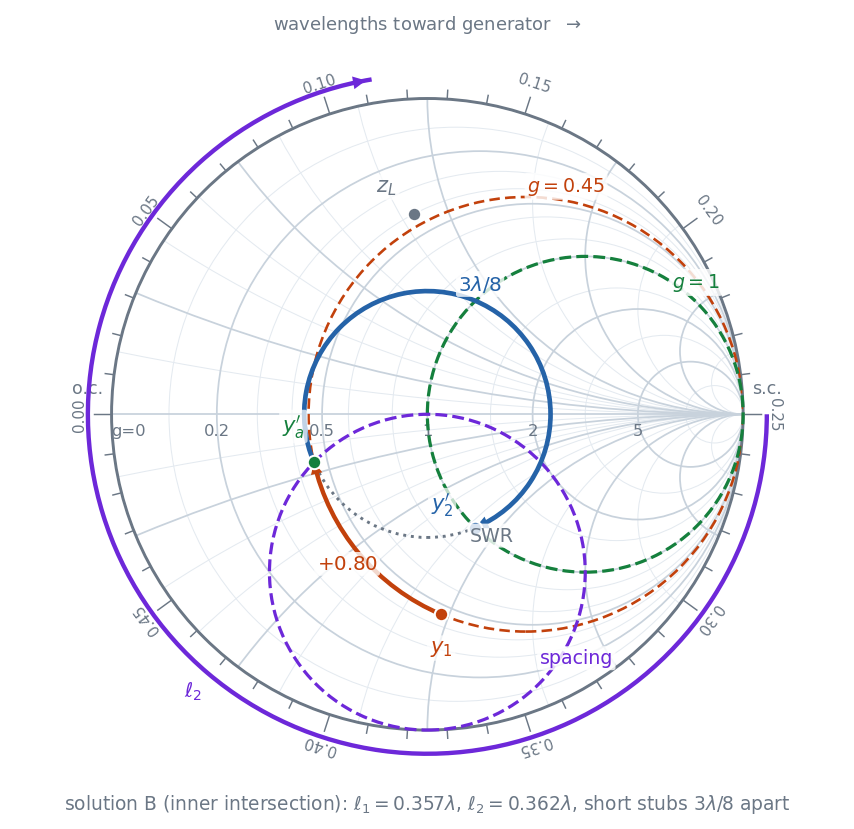
\includegraphics[width=0.495\textwidth]{figs/c2num_p14b.png}
\end{center}
{\footnotesize\color{sub} Problem 14 --- Smith chart construction, left: solution A, the outer intersection of the $g = 0.45$ circle with the spacing circle; right: solution B, the inner intersection of the $g = 0.45$ circle with the spacing circle.}

\figC{c2num_p14_line.png}{0.62\textwidth}
{\footnotesize\color{sub} Problem 14 --- line diagram of the matched network: shunt stubs across the line, lengths from the answer above.}

\figC{c2num_p14_coax.png}{0.69\textwidth}
{\footnotesize\color{sub} Problem 14 --- coaxial realisation, longitudinal section: each stub a coax tee off the main line; a shorting plate closes each stub.}

\penalty0\vspace{2pt}

%======================================================================
\Q{Problem 15 --- Double-stub shunt tuner}{\m{8}\m{2}}
{\color{sub}\footnotesize \yr{\texttt{80 Ba}} \gap$\cdot$\gap $Z_0 = 50\,\Omega$}

\begin{asked}{\texttt{80 Ba} \ [8+2]}
Design a double-stub shunt tuner using open stubs, $3\lambda/8$ apart, the first $0.4\lambda$ from the load, for $Z_L = 60-j80\,\Omega$ on a $50\,\Omega$ line. Prepare the S-matrix.
\end{asked}
\lead{Given}
\begin{itemize}
  \item $Z_L = 60.00 - j80.00\,\Omega$, $Z_0 = 50\,\Omega$.
\end{itemize}
\lead{Step 1 --- normalise and plot $z_L$}
\begin{itemize}
  \item $z_L = Z_L/Z_0 = 60.00 - j80.00$ over $50$ $=1.20 - j1.60$.
  \item Plot it where the $r = 1.20$ circle cuts the $x = -1.60$ arc; it reads $0.315\lambda$ on the WTG scale.
  \item Dividers from centre to $z_L$ (the SWR-circle radius), laid on the radially scaled scales below the chart: $|\Gamma_L| = 0.593$ on \emph{refl.\ coeff.\ E or I}, $S = 3.91$ on \emph{SWR}. \textit{Check:} $(z_L-1)/(z_L+1) = 0.593\angle -46.8^\circ$, $(1+|\Gamma_L|)/(1-|\Gamma_L|) = 3.91$.
\end{itemize}
\lead{Step 2 --- convert to admittance}
\begin{itemize}
  \item Draw the diameter through $z_L$ and read the opposite intersection --- a $\lambda/4$ half-turn. On an immittance chart read the amber grid in place and skip this step.
  \item $y_L = 1/z_L = 0.30 + j0.40$, at $0.065\lambda$ on the WTG scale (exactly $0.25\lambda$ from $z_L$).
\end{itemize}
\lead{Step 3 --- walk to the first stub}
\begin{itemize}
  \item The first stub sits $0.400\lambda$ from the load, so rotate $y_L$ \textbf{clockwise} that far along the SWR circle.
  \item $y_1 = 0.27 - j0.21$ at $0.465\lambda$ WTG --- the admittance seen \emph{just before} stub 1.
\end{itemize}
\lead{Step 4 --- draw the spacing circle}
\begin{itemize}
  \item Rotate the $g=1$ circle $3\lambda/8$ \textbf{toward the load} (anticlockwise). Call the result the \textbf{spacing circle}.
  \item Any point on it is carried \emph{onto} $g=1$ by the $3\lambda/8$ of line between the two stubs --- which is exactly what stub 1 must aim for.
  \item Check the forbidden region first: matching needs $g_1 \le 1/\sin^2\beta d = 2.00$, and here $g_1 = 0.268$. \checkmark
\end{itemize}
\lead{Step 5 --- stub 1: slide along the constant-$g$ circle}
\begin{itemize}
  \item A shunt stub adds susceptance only, so the point can move \emph{only along its own $g = 0.268$ circle}.
  \item Follow that circle to where it cuts the spacing circle. It cuts twice, giving the two standard solutions (one chart each below):
  \begin{itemize}
    \item \textbf{Solution A} (outer intersection, nearer the rim): $y_a = 0.27 - j1.68$, so stub 1 must add $b_1 = -1.681 - (-0.208) = -1.473$.
    \item \textbf{Solution B} (inner intersection, nearer the centre): $y_a' = 0.27 - j0.32$, so $b_1' = -0.111$.
  \end{itemize}
  \item Read $\ell_1$ off the rim, starting at the open-circuit point ($y=0$, the left of the chart): $\ell_1 = 0.345\lambda$ (A) and $0.482\lambda$ (B).
\end{itemize}
\lead{Step 6 --- the $3\lambda/8$ of line between the stubs}
\begin{itemize}
  \item Swing a \emph{new} SWR circle through $y_a$ and rotate \textbf{clockwise} by $3\lambda/8$.
  \item By construction it lands on the $g=1$ circle: $y_2 = 1.00 + j3.54$ (A), $y_2' = 1.00 - j1.54$ (B).
\end{itemize}
\lead{Step 7 --- stub 2 cancels what is left}
\begin{itemize}
  \item Stub 2 supplies $b_2 = -3.545$ (A) or $+1.545$ (B), leaving $y_{in} = 1 + j0$, i.e. $Z_{in} = Z_0 = 50\,\Omega$. Matched.
  \item Off the rim from the open-circuit point ($y=0$, the left of the chart): $\ell_2 = 0.294\lambda$ (A) and $0.159\lambda$ (B).
\end{itemize}
\lead{Answer}
\begin{tabularx}{\linewidth}{@{}L{3.2cm}X X@{}}
\toprule
\hrow \thead{Quantity} & \thead{Solution A} & \thead{Solution B} \\
\midrule
Stub spacing $d$ & $3\lambda/8$ & $3\lambda/8$ \\
First stub from load & $0.400\lambda$ & $0.400\lambda$ \\
$y$ before stub 1 & $0.27 - j0.21$ & $0.27 - j0.21$ \\
Stub 1 susceptance $b_1$ & $-1.473$ & $-0.111$ \\
\textbf{Stub 1 length $\ell_1$} & $0.345\lambda$ & $0.482\lambda$ \\
$y$ after the spacing & $1.00 + j3.54$ & $1.00 - j1.54$ \\
Stub 2 susceptance $b_2$ & $-3.545$ & $+1.545$ \\
\textbf{Stub 2 length $\ell_2$} & $0.294\lambda$ & $0.159\lambda$ \\
\bottomrule
\end{tabularx}

\lead{Both are correct.} Quote either, but say which you chose. Solution A uses the shorter stubs here, which is the practical pick: less line at high VSWR means lower loss and wider bandwidth.
\lead{S-matrix before and after matching}
\begin{itemize}
  \item \textbf{Before} --- the bare load is a one-port, so $[S] = [\Gamma_L] = [0.593\angle -46.8^\circ]$, with $S = 3.91$.
  \item \textbf{After} --- the tuner makes $Z_{in} = Z_0$, so $S_{11} = S_{22} = 0$. The network is passive and reciprocal ($S_{12} = S_{21}$) and lossless, so unitarity forces $|S_{21}| = 1$:
\  \[ [S] = \begin{bmatrix} 0 & 1 \\ 1 & 0 \end{bmatrix} \quad \text{or} \quad \begin{bmatrix} 0 & e^{-j\theta} \\ e^{-j\theta} & 0 \end{bmatrix} \]
  \item Keeping the $e^{-j\theta}$ records the through-path electrical length; either form earns the marks if you say which you mean.
\end{itemize}

\begin{center}
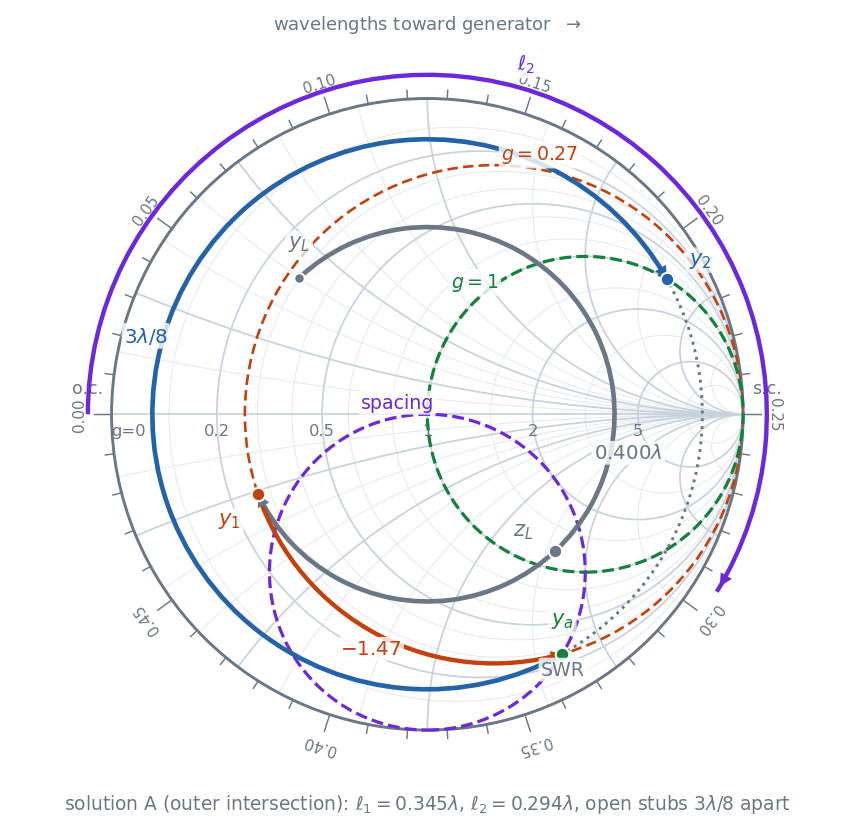
\includegraphics[width=0.495\textwidth]{figs/c2num_p15.png}\hfill
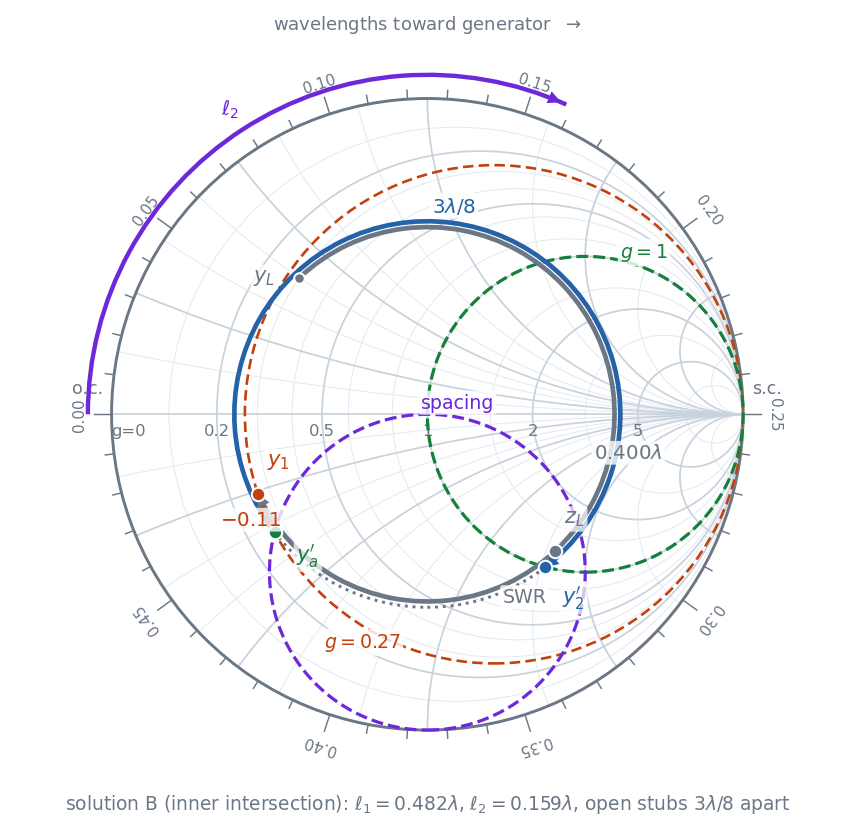
\includegraphics[width=0.495\textwidth]{figs/c2num_p15b.png}
\end{center}
{\footnotesize\color{sub} Problem 15 --- Smith chart construction, left: solution A, the outer intersection of the $g = 0.27$ circle with the spacing circle; right: solution B, the inner intersection of the $g = 0.27$ circle with the spacing circle.}

\figC{c2num_p15_line.png}{0.62\textwidth}
{\footnotesize\color{sub} Problem 15 --- line diagram of the matched network: shunt stubs across the line, lengths from the answer above.}

\figC{c2num_p15_coax.png}{0.92\textwidth}
{\footnotesize\color{sub} Problem 15 --- coaxial realisation, longitudinal section: each stub a coax tee off the main line; each stub's centre conductor stops short of an open end.}

\penalty0\vspace{2pt}

%======================================================================
\Q{Problem 16 --- Double-stub shunt tuner}{\m{8}\m{2}}
{\color{sub}\footnotesize \yr{\textbf{\texttt{80 Bh}}} \gap$\cdot$\gap $Z_0 = 75\,\Omega$}

\begin{asked}{\textbf{\texttt{80 Bh}} \ [8+2]}
Design a short-circuited double-stub tuner on a $75\,\Omega$ coaxial line for $Z_L = 109+j120\,\Omega$. Prepare the S-matrix.
\end{asked}
\lead{Given}
\begin{itemize}
  \item $Z_L = 109.00 + j120.00\,\Omega$, $Z_0 = 75\,\Omega$.
\end{itemize}
\lead{Step 1 --- normalise and plot $z_L$}
\begin{itemize}
  \item $z_L = Z_L/Z_0 = 109.00 + j120.00$ over $75$ $=1.45 + j1.60$.
  \item Plot it where the $r = 1.45$ circle cuts the $x = +1.60$ arc; it reads $0.193\lambda$ on the WTG scale.
  \item Dividers from centre to $z_L$ (the SWR-circle radius), laid on the radially scaled scales below the chart: $|\Gamma_L| = 0.568$ on \emph{refl.\ coeff.\ E or I}, $S = 3.63$ on \emph{SWR}. \textit{Check:} $(z_L-1)/(z_L+1) = 0.568\angle 41.1^\circ$, $(1+|\Gamma_L|)/(1-|\Gamma_L|) = 3.63$.
\end{itemize}
\lead{Step 2 --- convert to admittance}
\begin{itemize}
  \item Draw the diameter through $z_L$ and read the opposite intersection --- a $\lambda/4$ half-turn. On an immittance chart read the amber grid in place and skip this step.
  \item $y_L = 1/z_L = 0.31 - j0.34$, at $0.443\lambda$ on the WTG scale (exactly $0.25\lambda$ from $z_L$).
\end{itemize}
\lead{Step 3 --- the first stub is at the load}
\begin{itemize}
  \item No offset is specified, so stub 1 sits at the load and $y_1 = y_L = 0.31 - j0.34$.
\end{itemize}
\lead{Step 4 --- draw the spacing circle}
\begin{itemize}
  \item Rotate the $g=1$ circle $3\lambda/8$ \textbf{toward the load} (anticlockwise). Call the result the \textbf{spacing circle}.
  \item Any point on it is carried \emph{onto} $g=1$ by the $3\lambda/8$ of line between the two stubs --- which is exactly what stub 1 must aim for.
  \item Check the forbidden region first: matching needs $g_1 \le 1/\sin^2\beta d = 2.00$, and here $g_1 = 0.311$. \checkmark
\end{itemize}
\lead{Step 5 --- stub 1: slide along the constant-$g$ circle}
\begin{itemize}
  \item A shunt stub adds susceptance only, so the point can move \emph{only along its own $g = 0.311$ circle}.
  \item Follow that circle to where it cuts the spacing circle. It cuts twice, giving the two standard solutions (one chart each below):
  \begin{itemize}
    \item \textbf{Solution A} (outer intersection, nearer the rim): $y_a = 0.31 - j1.72$, so stub 1 must add $b_1 = -1.725 - (-0.342) = -1.382$.
    \item \textbf{Solution B} (inner intersection, nearer the centre): $y_a' = 0.31 - j0.28$, so $b_1' = +0.067$.
  \end{itemize}
  \item Read $\ell_1$ off the rim, starting at the short-circuit point ($y=\infty$, the right of the chart): $\ell_1 = 0.100\lambda$ (A) and $0.261\lambda$ (B).
\end{itemize}
\lead{Step 6 --- the $3\lambda/8$ of line between the stubs}
\begin{itemize}
  \item Swing a \emph{new} SWR circle through $y_a$ and rotate \textbf{clockwise} by $3\lambda/8$.
  \item By construction it lands on the $g=1$ circle: $y_2 = 1.00 + j3.33$ (A), $y_2' = 1.00 - j1.33$ (B).
\end{itemize}
\lead{Step 7 --- stub 2 cancels what is left}
\begin{itemize}
  \item Stub 2 supplies $b_2 = -3.330$ (A) or $+1.330$ (B), leaving $y_{in} = 1 + j0$, i.e. $Z_{in} = Z_0 = 75\,\Omega$. Matched.
  \item Off the rim from the short-circuit point ($y=\infty$, the right of the chart): $\ell_2 = 0.046\lambda$ (A) and $0.397\lambda$ (B).
\end{itemize}
\lead{Answer}
\begin{tabularx}{\linewidth}{@{}L{3.2cm}X X@{}}
\toprule
\hrow \thead{Quantity} & \thead{Solution A} & \thead{Solution B} \\
\midrule
Stub spacing $d$ & $3\lambda/8$ & $3\lambda/8$ \\
First stub from load & $0.000\lambda$ & $0.000\lambda$ \\
$y$ before stub 1 & $0.31 - j0.34$ & $0.31 - j0.34$ \\
Stub 1 susceptance $b_1$ & $-1.382$ & $+0.067$ \\
\textbf{Stub 1 length $\ell_1$} & $0.100\lambda$ & $0.261\lambda$ \\
$y$ after the spacing & $1.00 + j3.33$ & $1.00 - j1.33$ \\
Stub 2 susceptance $b_2$ & $-3.330$ & $+1.330$ \\
\textbf{Stub 2 length $\ell_2$} & $0.046\lambda$ & $0.397\lambda$ \\
\bottomrule
\end{tabularx}

\lead{Both are correct.} Quote either, but say which you chose. Solution A uses the shorter stubs here, which is the practical pick: less line at high VSWR means lower loss and wider bandwidth.
\lead{S-matrix before and after matching}
\begin{itemize}
  \item \textbf{Before} --- the bare load is a one-port, so $[S] = [\Gamma_L] = [0.568\angle 41.1^\circ]$, with $S = 3.63$.
  \item \textbf{After} --- the tuner makes $Z_{in} = Z_0$, so $S_{11} = S_{22} = 0$. The network is passive and reciprocal ($S_{12} = S_{21}$) and lossless, so unitarity forces $|S_{21}| = 1$:
\  \[ [S] = \begin{bmatrix} 0 & 1 \\ 1 & 0 \end{bmatrix} \quad \text{or} \quad \begin{bmatrix} 0 & e^{-j\theta} \\ e^{-j\theta} & 0 \end{bmatrix} \]
  \item Keeping the $e^{-j\theta}$ records the through-path electrical length; either form earns the marks if you say which you mean.
\end{itemize}

\begin{center}
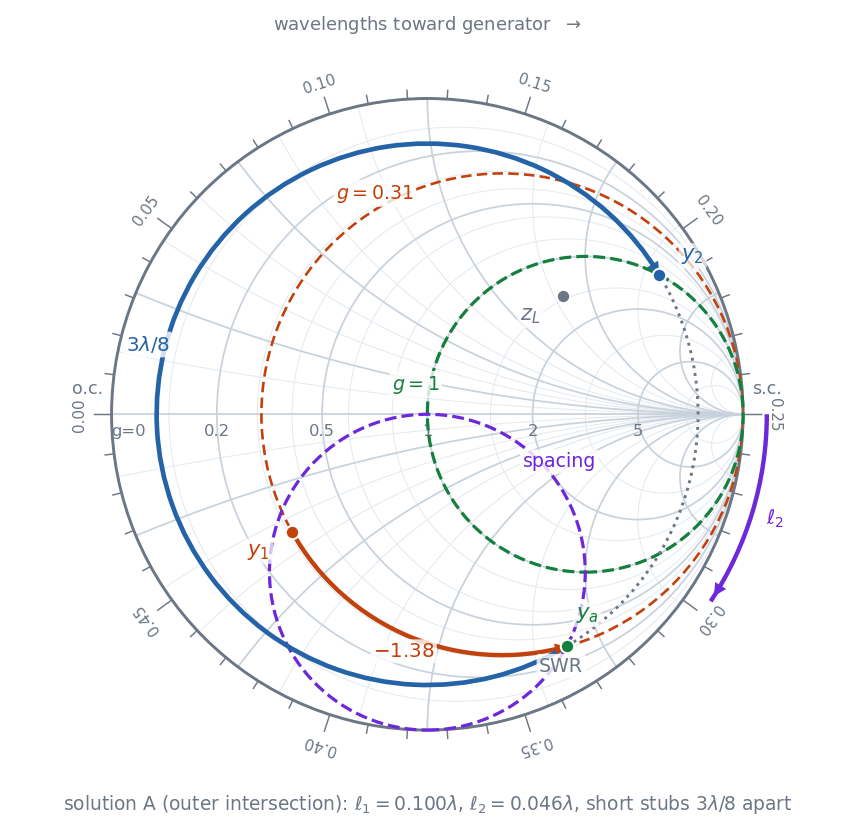
\includegraphics[width=0.495\textwidth]{figs/c2num_p16.png}\hfill
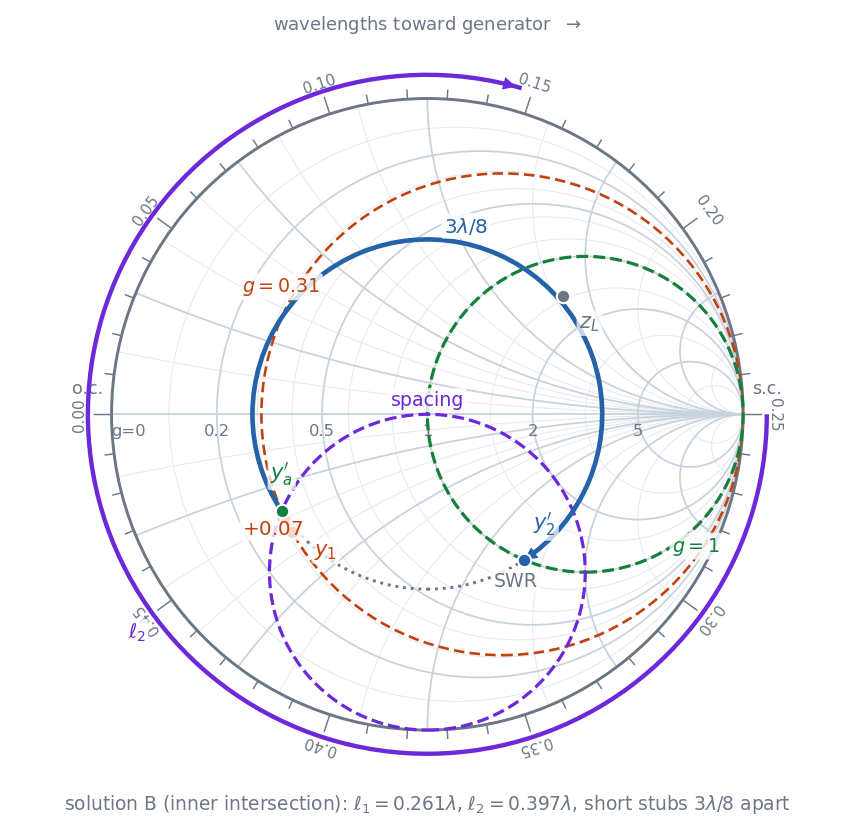
\includegraphics[width=0.495\textwidth]{figs/c2num_p16b.png}
\end{center}
{\footnotesize\color{sub} Problem 16 --- Smith chart construction, left: solution A, the outer intersection of the $g = 0.31$ circle with the spacing circle; right: solution B, the inner intersection of the $g = 0.31$ circle with the spacing circle.}

\figC{c2num_p16_line.png}{0.62\textwidth}
{\footnotesize\color{sub} Problem 16 --- line diagram of the matched network: shunt stubs across the line, lengths from the answer above.}

\figC{c2num_p16_coax.png}{0.69\textwidth}
{\footnotesize\color{sub} Problem 16 --- coaxial realisation, longitudinal section: each stub a coax tee off the main line; a shorting plate closes each stub.}

\penalty0\vspace{2pt}

%======================================================================
\Q{Problem 17 --- Double-stub shunt tuner}{\m{8}\m{2}}
{\color{sub}\footnotesize \yr{\texttt{81 Ba}} \gap$\cdot$\gap $Z_0 = 100\,\Omega$}

\begin{asked}{\texttt{81 Ba} \ [8+2]}
A load presents $\Gamma_L = 0.64\angle 58^\circ$ on a $100\,\Omega$ line. Design a double-stub tuner and prepare the S-matrix of the matched network.
\end{asked}
\lead{Given}
\begin{itemize}
  \item $\Gamma_L = 0.640\angle 58.0^\circ$, $Z_0 = 100\,\Omega$ $\Rightarrow$ $Z_L = Z_0(1+\Gamma_L)/(1-\Gamma_L) = 80.73 + j148.43\,\Omega$.
\end{itemize}
\lead{Step 1 --- normalise and plot $z_L$}
\begin{itemize}
  \item $z_L = Z_L/Z_0 = 80.73 + j148.43$ over $100$ $=0.81 + j1.48$.
  \item Plot it where the $r = 0.81$ circle cuts the $x = +1.48$ arc; it reads $0.169\lambda$ on the WTG scale.
  \item Dividers from centre to $z_L$ (the SWR-circle radius), laid on the radially scaled scales below the chart: $|\Gamma_L| = 0.640$ on \emph{refl.\ coeff.\ E or I}, $S = 4.56$ on \emph{SWR}. \textit{Check:} $(z_L-1)/(z_L+1) = 0.640\angle 58.0^\circ$, $(1+|\Gamma_L|)/(1-|\Gamma_L|) = 4.56$.
\end{itemize}
\lead{Step 2 --- convert to admittance}
\begin{itemize}
  \item Draw the diameter through $z_L$ and read the opposite intersection --- a $\lambda/4$ half-turn. On an immittance chart read the amber grid in place and skip this step.
  \item $y_L = 1/z_L = 0.28 - j0.52$, at $0.419\lambda$ on the WTG scale (exactly $0.25\lambda$ from $z_L$).
\end{itemize}
\lead{Step 3 --- the first stub is at the load}
\begin{itemize}
  \item No offset is specified, so stub 1 sits at the load and $y_1 = y_L = 0.28 - j0.52$.
\end{itemize}
\lead{Step 4 --- draw the spacing circle}
\begin{itemize}
  \item Rotate the $g=1$ circle $3\lambda/8$ \textbf{toward the load} (anticlockwise). Call the result the \textbf{spacing circle}.
  \item Any point on it is carried \emph{onto} $g=1$ by the $3\lambda/8$ of line between the two stubs --- which is exactly what stub 1 must aim for.
  \item Check the forbidden region first: matching needs $g_1 \le 1/\sin^2\beta d = 2.00$, and here $g_1 = 0.283$. \checkmark
\end{itemize}
\lead{Step 5 --- stub 1: slide along the constant-$g$ circle}
\begin{itemize}
  \item A shunt stub adds susceptance only, so the point can move \emph{only along its own $g = 0.283$ circle}.
  \item Follow that circle to where it cuts the spacing circle. It cuts twice, giving the two standard solutions (one chart each below):
  \begin{itemize}
    \item \textbf{Solution A} (outer intersection, nearer the rim): $y_a = 0.28 - j1.70$, so stub 1 must add $b_1 = -1.697 - (-0.520) = -1.177$.
    \item \textbf{Solution B} (inner intersection, nearer the centre): $y_a' = 0.28 - j0.30$, so $b_1' = +0.217$.
  \end{itemize}
  \item Read $\ell_1$ off the rim, starting at the short-circuit point ($y=\infty$, the right of the chart): $\ell_1 = 0.112\lambda$ (A) and $0.284\lambda$ (B).
\end{itemize}
\lead{Step 6 --- the $3\lambda/8$ of line between the stubs}
\begin{itemize}
  \item Swing a \emph{new} SWR circle through $y_a$ and rotate \textbf{clockwise} by $3\lambda/8$.
  \item By construction it lands on the $g=1$ circle: $y_2 = 1.00 + j3.46$ (A), $y_2' = 1.00 - j1.46$ (B).
\end{itemize}
\lead{Step 7 --- stub 2 cancels what is left}
\begin{itemize}
  \item Stub 2 supplies $b_2 = -3.464$ (A) or $+1.464$ (B), leaving $y_{in} = 1 + j0$, i.e. $Z_{in} = Z_0 = 100\,\Omega$. Matched.
  \item Off the rim from the short-circuit point ($y=\infty$, the right of the chart): $\ell_2 = 0.045\lambda$ (A) and $0.405\lambda$ (B).
\end{itemize}
\lead{Answer}
\begin{tabularx}{\linewidth}{@{}L{3.2cm}X X@{}}
\toprule
\hrow \thead{Quantity} & \thead{Solution A} & \thead{Solution B} \\
\midrule
Stub spacing $d$ & $3\lambda/8$ & $3\lambda/8$ \\
First stub from load & $0.000\lambda$ & $0.000\lambda$ \\
$y$ before stub 1 & $0.28 - j0.52$ & $0.28 - j0.52$ \\
Stub 1 susceptance $b_1$ & $-1.177$ & $+0.217$ \\
\textbf{Stub 1 length $\ell_1$} & $0.112\lambda$ & $0.284\lambda$ \\
$y$ after the spacing & $1.00 + j3.46$ & $1.00 - j1.46$ \\
Stub 2 susceptance $b_2$ & $-3.464$ & $+1.464$ \\
\textbf{Stub 2 length $\ell_2$} & $0.045\lambda$ & $0.405\lambda$ \\
\bottomrule
\end{tabularx}

\lead{Both are correct.} Quote either, but say which you chose. Solution A uses the shorter stubs here, which is the practical pick: less line at high VSWR means lower loss and wider bandwidth.
\lead{S-matrix before and after matching}
\begin{itemize}
  \item \textbf{Before} --- the bare load is a one-port, so $[S] = [\Gamma_L] = [0.640\angle 58.0^\circ]$, with $S = 4.56$.
  \item \textbf{After} --- the tuner makes $Z_{in} = Z_0$, so $S_{11} = S_{22} = 0$. The network is passive and reciprocal ($S_{12} = S_{21}$) and lossless, so unitarity forces $|S_{21}| = 1$:
\  \[ [S] = \begin{bmatrix} 0 & 1 \\ 1 & 0 \end{bmatrix} \quad \text{or} \quad \begin{bmatrix} 0 & e^{-j\theta} \\ e^{-j\theta} & 0 \end{bmatrix} \]
  \item Keeping the $e^{-j\theta}$ records the through-path electrical length; either form earns the marks if you say which you mean.
\end{itemize}

\begin{center}
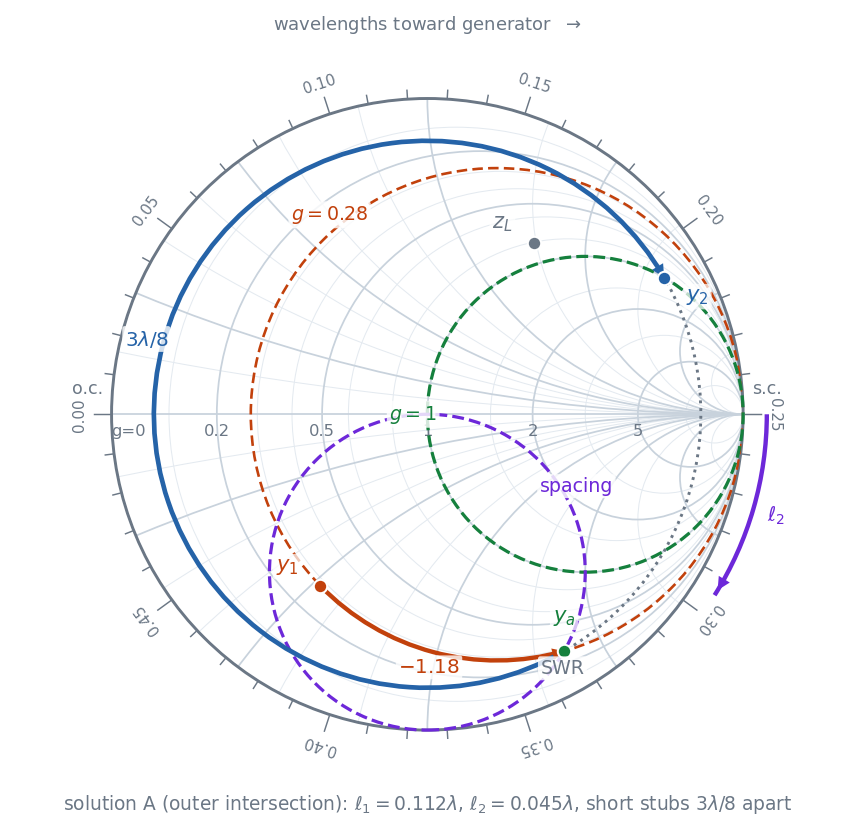
\includegraphics[width=0.495\textwidth]{figs/c2num_p17.png}\hfill
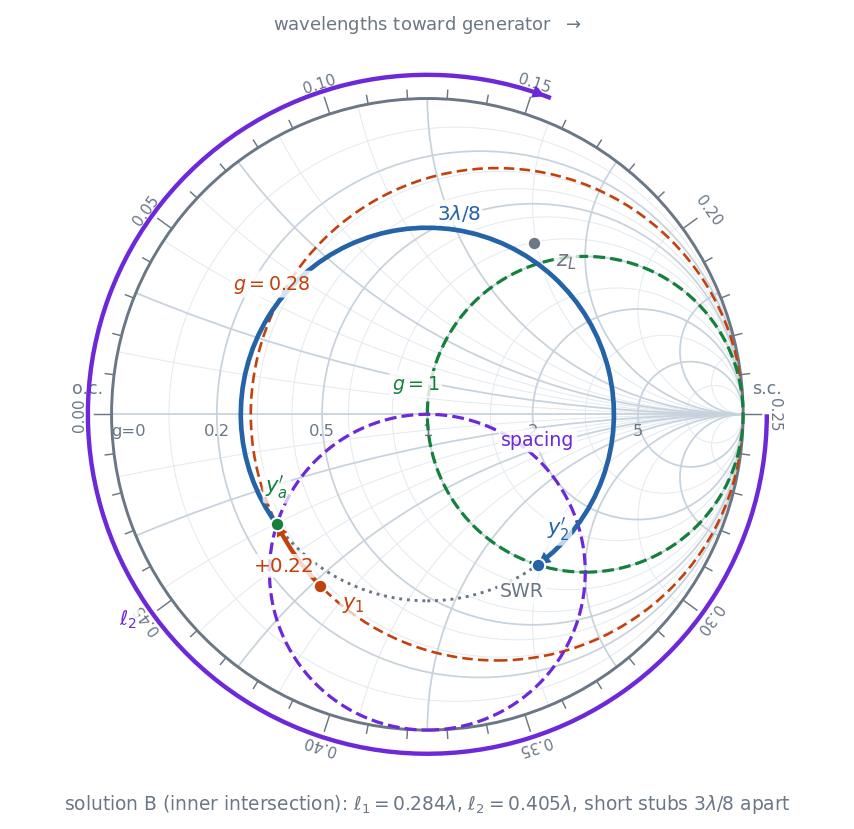
\includegraphics[width=0.495\textwidth]{figs/c2num_p17b.png}
\end{center}
{\footnotesize\color{sub} Problem 17 --- Smith chart construction, left: solution A, the outer intersection of the $g = 0.28$ circle with the spacing circle; right: solution B, the inner intersection of the $g = 0.28$ circle with the spacing circle.}

\figC{c2num_p17_line.png}{0.62\textwidth}
{\footnotesize\color{sub} Problem 17 --- line diagram of the matched network: shunt stubs across the line, lengths from the answer above.}

\figC{c2num_p17_coax.png}{0.69\textwidth}
{\footnotesize\color{sub} Problem 17 --- coaxial realisation, longitudinal section: each stub a coax tee off the main line; a shorting plate closes each stub.}

\penalty0\vspace{2pt}

%======================================================================
\Q{Problem 18 --- Double-stub shunt tuner}{\m{8}\m{2}}
{\color{sub}\footnotesize \yr{\textbf{\texttt{79 Bh}}} \gap$\cdot$\gap $Z_0 = 50\,\Omega$}

\begin{asked}{\textbf{\texttt{79 Bh}} \ [8+2]}
A $50\,\Omega$ lossless line feeds a load of admittance $0.00813+j0.0065\,\mho$. Design a double-stub shunt tuner ($3\lambda/8$ spacing, first stub $0.01\lambda$ from the load) using the Smith chart and write the S-parameters.
\end{asked}
\lead{Given}
\begin{itemize}
  \item $Y_L = 0.00813 + j0.00650\,\mho$ $\Rightarrow$ $Z_L = 1/Y_L = 75.04 - j59.99\,\Omega$.
\end{itemize}
\lead{Step 1 --- normalise and plot $z_L$}
\begin{itemize}
  \item $z_L = Z_L/Z_0 = 75.04 - j59.99$ over $50$ $=1.50 - j1.20$.
  \item Plot it where the $r = 1.50$ circle cuts the $x = -1.20$ arc; it reads $0.308\lambda$ on the WTG scale.
  \item Dividers from centre to $z_L$ (the SWR-circle radius), laid on the radially scaled scales below the chart: $|\Gamma_L| = 0.469$ on \emph{refl.\ coeff.\ E or I}, $S = 2.76$ on \emph{SWR}. \textit{Check:} $(z_L-1)/(z_L+1) = 0.469\angle -41.7^\circ$, $(1+|\Gamma_L|)/(1-|\Gamma_L|) = 2.76$.
\end{itemize}
\lead{Step 2 --- convert to admittance}
\begin{itemize}
  \item Draw the diameter through $z_L$ and read the opposite intersection --- a $\lambda/4$ half-turn. On an immittance chart read the amber grid in place and skip this step.
  \item $y_L = 1/z_L = 0.41 + j0.32$, at $0.058\lambda$ on the WTG scale (exactly $0.25\lambda$ from $z_L$).
\end{itemize}
\lead{Step 3 --- walk to the first stub}
\begin{itemize}
  \item The first stub sits $0.010\lambda$ from the load, so rotate $y_L$ \textbf{clockwise} that far along the SWR circle.
  \item $y_1 = 0.43 + j0.38$ at $0.068\lambda$ WTG --- the admittance seen \emph{just before} stub 1.
\end{itemize}
\lead{Step 4 --- draw the spacing circle}
\begin{itemize}
  \item Rotate the $g=1$ circle $3\lambda/8$ \textbf{toward the load} (anticlockwise). Call the result the \textbf{spacing circle}.
  \item Any point on it is carried \emph{onto} $g=1$ by the $3\lambda/8$ of line between the two stubs --- which is exactly what stub 1 must aim for.
  \item Check the forbidden region first: matching needs $g_1 \le 1/\sin^2\beta d = 2.00$, and here $g_1 = 0.425$. \checkmark
\end{itemize}
\lead{Step 5 --- stub 1: slide along the constant-$g$ circle}
\begin{itemize}
  \item A shunt stub adds susceptance only, so the point can move \emph{only along its own $g = 0.425$ circle}.
  \item Follow that circle to where it cuts the spacing circle. It cuts twice, giving the two standard solutions (one chart each below):
  \begin{itemize}
    \item \textbf{Solution A} (outer intersection, nearer the rim): $y_a = 0.43 - j1.82$, so stub 1 must add $b_1 = -1.818 - (0.385) = -2.203$.
    \item \textbf{Solution B} (inner intersection, nearer the centre): $y_a' = 0.43 - j0.18$, so $b_1' = -0.567$.
  \end{itemize}
  \item Read $\ell_1$ off the rim, starting at the short-circuit point ($y=\infty$, the right of the chart): $\ell_1 = 0.068\lambda$ (A) and $0.168\lambda$ (B).
\end{itemize}
\lead{Step 6 --- the $3\lambda/8$ of line between the stubs}
\begin{itemize}
  \item Swing a \emph{new} SWR circle through $y_a$ and rotate \textbf{clockwise} by $3\lambda/8$.
  \item By construction it lands on the $g=1$ circle: $y_2 = 1.00 + j2.92$ (A), $y_2' = 1.00 - j0.92$ (B).
\end{itemize}
\lead{Step 7 --- stub 2 cancels what is left}
\begin{itemize}
  \item Stub 2 supplies $b_2 = -2.925$ (A) or $+0.925$ (B), leaving $y_{in} = 1 + j0$, i.e. $Z_{in} = Z_0 = 50\,\Omega$. Matched.
  \item Off the rim from the short-circuit point ($y=\infty$, the right of the chart): $\ell_2 = 0.052\lambda$ (A) and $0.369\lambda$ (B).
\end{itemize}
\lead{Answer}
\begin{tabularx}{\linewidth}{@{}L{3.2cm}X X@{}}
\toprule
\hrow \thead{Quantity} & \thead{Solution A} & \thead{Solution B} \\
\midrule
Stub spacing $d$ & $3\lambda/8$ & $3\lambda/8$ \\
First stub from load & $0.010\lambda$ & $0.010\lambda$ \\
$y$ before stub 1 & $0.43 + j0.38$ & $0.43 + j0.38$ \\
Stub 1 susceptance $b_1$ & $-2.203$ & $-0.567$ \\
\textbf{Stub 1 length $\ell_1$} & $0.068\lambda$ & $0.168\lambda$ \\
$y$ after the spacing & $1.00 + j2.92$ & $1.00 - j0.92$ \\
Stub 2 susceptance $b_2$ & $-2.925$ & $+0.925$ \\
\textbf{Stub 2 length $\ell_2$} & $0.052\lambda$ & $0.369\lambda$ \\
\bottomrule
\end{tabularx}

\lead{Both are correct.} Quote either, but say which you chose. Solution A uses the shorter stubs here, which is the practical pick: less line at high VSWR means lower loss and wider bandwidth.
\lead{S-matrix before and after matching}
\begin{itemize}
  \item \textbf{Before} --- the bare load is a one-port, so $[S] = [\Gamma_L] = [0.469\angle -41.7^\circ]$, with $S = 2.76$.
  \item \textbf{After} --- the tuner makes $Z_{in} = Z_0$, so $S_{11} = S_{22} = 0$. The network is passive and reciprocal ($S_{12} = S_{21}$) and lossless, so unitarity forces $|S_{21}| = 1$:
\  \[ [S] = \begin{bmatrix} 0 & 1 \\ 1 & 0 \end{bmatrix} \quad \text{or} \quad \begin{bmatrix} 0 & e^{-j\theta} \\ e^{-j\theta} & 0 \end{bmatrix} \]
  \item Keeping the $e^{-j\theta}$ records the through-path electrical length; either form earns the marks if you say which you mean.
\end{itemize}

\begin{center}
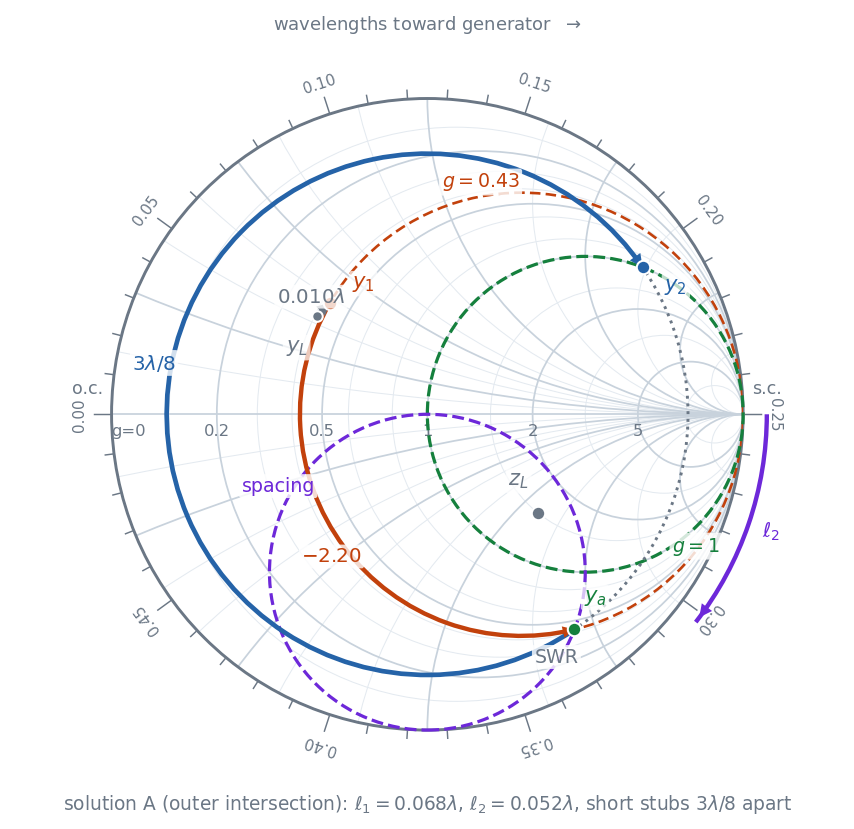
\includegraphics[width=0.495\textwidth]{figs/c2num_p18.png}\hfill
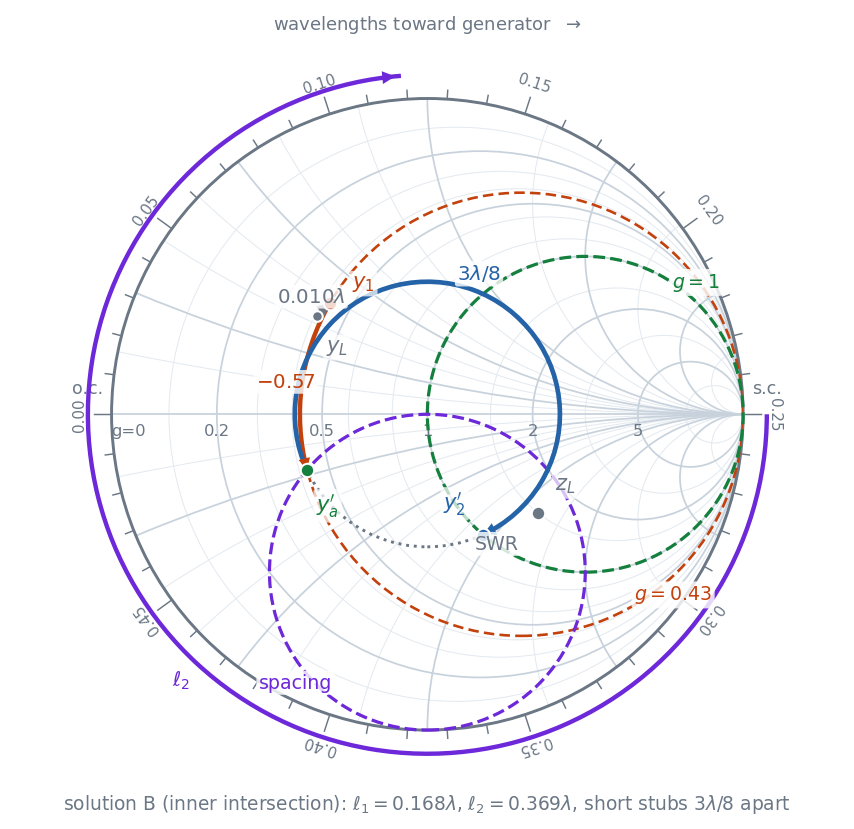
\includegraphics[width=0.495\textwidth]{figs/c2num_p18b.png}
\end{center}
{\footnotesize\color{sub} Problem 18 --- Smith chart construction, left: solution A, the outer intersection of the $g = 0.43$ circle with the spacing circle; right: solution B, the inner intersection of the $g = 0.43$ circle with the spacing circle.}

\figC{c2num_p18_line.png}{0.62\textwidth}
{\footnotesize\color{sub} Problem 18 --- line diagram of the matched network: shunt stubs across the line, lengths from the answer above.}

\figC{c2num_p18_coax.png}{0.70\textwidth}
{\footnotesize\color{sub} Problem 18 --- coaxial realisation, longitudinal section: each stub a coax tee off the main line; a shorting plate closes each stub.}

\penalty0\vspace{2pt}

%======================================================================
\Q{Problem 19 --- Double-stub shunt tuner}{\m{10}}
{\color{sub}\footnotesize \yr{\textbf{\texttt{82 Bh}}} \gap$\cdot$\gap $Z_0 = 75\,\Omega$}

\begin{asked}{\textbf{\texttt{82 Bh}} \ [10]}
A broadband microstrip antenna has load reflection coefficient $0.33\angle 66^\circ$ on a $75\,\Omega$ transmission patch. Design the matching stubs and express the scattering matrix of the matched network.
\end{asked}
\lead{Given}
\begin{itemize}
  \item $\Gamma_L = 0.330\angle 66.0^\circ$, $Z_0 = 75\,\Omega$ $\Rightarrow$ $Z_L = Z_0(1+\Gamma_L)/(1-\Gamma_L) = 79.52 + j53.80\,\Omega$.
\end{itemize}
\lead{Step 1 --- normalise and plot $z_L$}
\begin{itemize}
  \item $z_L = Z_L/Z_0 = 79.52 + j53.80$ over $75$ $=1.06 + j0.72$.
  \item Plot it where the $r = 1.06$ circle cuts the $x = +0.72$ arc; it reads $0.158\lambda$ on the WTG scale.
  \item Dividers from centre to $z_L$ (the SWR-circle radius), laid on the radially scaled scales below the chart: $|\Gamma_L| = 0.330$ on \emph{refl.\ coeff.\ E or I}, $S = 1.99$ on \emph{SWR}. \textit{Check:} $(z_L-1)/(z_L+1) = 0.330\angle 66.0^\circ$, $(1+|\Gamma_L|)/(1-|\Gamma_L|) = 1.99$.
\end{itemize}
\lead{Step 2 --- convert to admittance}
\begin{itemize}
  \item Draw the diameter through $z_L$ and read the opposite intersection --- a $\lambda/4$ half-turn. On an immittance chart read the amber grid in place and skip this step.
  \item $y_L = 1/z_L = 0.65 - j0.44$, at $0.408\lambda$ on the WTG scale (exactly $0.25\lambda$ from $z_L$).
\end{itemize}
\lead{Step 3 --- the first stub is at the load}
\begin{itemize}
  \item No offset is specified, so stub 1 sits at the load and $y_1 = y_L = 0.65 - j0.44$.
\end{itemize}
\lead{Step 4 --- draw the spacing circle}
\begin{itemize}
  \item Rotate the $g=1$ circle $3\lambda/8$ \textbf{toward the load} (anticlockwise). Call the result the \textbf{spacing circle}.
  \item Any point on it is carried \emph{onto} $g=1$ by the $3\lambda/8$ of line between the two stubs --- which is exactly what stub 1 must aim for.
  \item Check the forbidden region first: matching needs $g_1 \le 1/\sin^2\beta d = 2.00$, and here $g_1 = 0.647$. \checkmark
\end{itemize}
\lead{Step 5 --- stub 1: slide along the constant-$g$ circle}
\begin{itemize}
  \item A shunt stub adds susceptance only, so the point can move \emph{only along its own $g = 0.647$ circle}.
  \item Follow that circle to where it cuts the spacing circle. It cuts twice, giving the two standard solutions (one chart each below):
  \begin{itemize}
    \item \textbf{Solution A} (outer intersection, nearer the rim): $y_a = 0.65 - j1.94$, so stub 1 must add $b_1 = -1.936 - (-0.438) = -1.498$.
    \item \textbf{Solution B} (inner intersection, nearer the centre): $y_a' = 0.65 - j0.06$, so $b_1' = +0.373$.
  \end{itemize}
  \item Read $\ell_1$ off the rim, starting at the open-circuit point ($y=0$, the left of the chart): $\ell_1 = 0.344\lambda$ (A) and $0.057\lambda$ (B).
\end{itemize}
\lead{Step 6 --- the $3\lambda/8$ of line between the stubs}
\begin{itemize}
  \item Swing a \emph{new} SWR circle through $y_a$ and rotate \textbf{clockwise} by $3\lambda/8$.
  \item By construction it lands on the $g=1$ circle: $y_2 = 1.00 + j2.45$ (A), $y_2' = 1.00 - j0.45$ (B).
\end{itemize}
\lead{Step 7 --- stub 2 cancels what is left}
\begin{itemize}
  \item Stub 2 supplies $b_2 = -2.446$ (A) or $+0.446$ (B), leaving $y_{in} = 1 + j0$, i.e. $Z_{in} = Z_0 = 75\,\Omega$. Matched.
  \item Off the rim from the open-circuit point ($y=0$, the left of the chart): $\ell_2 = 0.312\lambda$ (A) and $0.067\lambda$ (B).
\end{itemize}
\lead{Answer}
\begin{tabularx}{\linewidth}{@{}L{3.2cm}X X@{}}
\toprule
\hrow \thead{Quantity} & \thead{Solution A} & \thead{Solution B} \\
\midrule
Stub spacing $d$ & $3\lambda/8$ & $3\lambda/8$ \\
First stub from load & $0.000\lambda$ & $0.000\lambda$ \\
$y$ before stub 1 & $0.65 - j0.44$ & $0.65 - j0.44$ \\
Stub 1 susceptance $b_1$ & $-1.498$ & $+0.373$ \\
\textbf{Stub 1 length $\ell_1$} & $0.344\lambda$ & $0.057\lambda$ \\
$y$ after the spacing & $1.00 + j2.45$ & $1.00 - j0.45$ \\
Stub 2 susceptance $b_2$ & $-2.446$ & $+0.446$ \\
\textbf{Stub 2 length $\ell_2$} & $0.312\lambda$ & $0.067\lambda$ \\
\bottomrule
\end{tabularx}

\lead{Both are correct.} Quote either, but say which you chose. Solution B uses the shorter stubs here, which is the practical pick: less line at high VSWR means lower loss and wider bandwidth.
\lead{S-matrix before and after matching}
\begin{itemize}
  \item \textbf{Before} --- the bare load is a one-port, so $[S] = [\Gamma_L] = [0.330\angle 66.0^\circ]$, with $S = 1.99$.
  \item \textbf{After} --- the tuner makes $Z_{in} = Z_0$, so $S_{11} = S_{22} = 0$. The network is passive and reciprocal ($S_{12} = S_{21}$) and lossless, so unitarity forces $|S_{21}| = 1$:
\  \[ [S] = \begin{bmatrix} 0 & 1 \\ 1 & 0 \end{bmatrix} \quad \text{or} \quad \begin{bmatrix} 0 & e^{-j\theta} \\ e^{-j\theta} & 0 \end{bmatrix} \]
  \item Keeping the $e^{-j\theta}$ records the through-path electrical length; either form earns the marks if you say which you mean.
\end{itemize}
\lead{Microstrip realisation}
\begin{itemize}
  \item Take FR-4, $\epsilon_r = 4.4$, $h = 1.6\text{ mm}$. Hammerstad synthesis for $75\,\Omega$ gives $W/h = 0.89$, i.e. $W = 1.43\text{ mm}$, with $\epsilon_e = 3.15$.
  \item No frequency is given, so leave the answers in wavelengths; multiply by $\lambda_g = \lambda_0/\sqrt{\epsilon_e}$ once $f$ is fixed.
  \item Draw the stubs as T-junctions off the $W$-wide main line. Open stubs are plain truncated strips (no via needed) --- which is why open stubs are preferred in microstrip.
  \item Shorten each open stub by the fringing allowance $\Delta\ell \approx 0.3h = 0.48\text{ mm}$.
\end{itemize}

\begin{center}
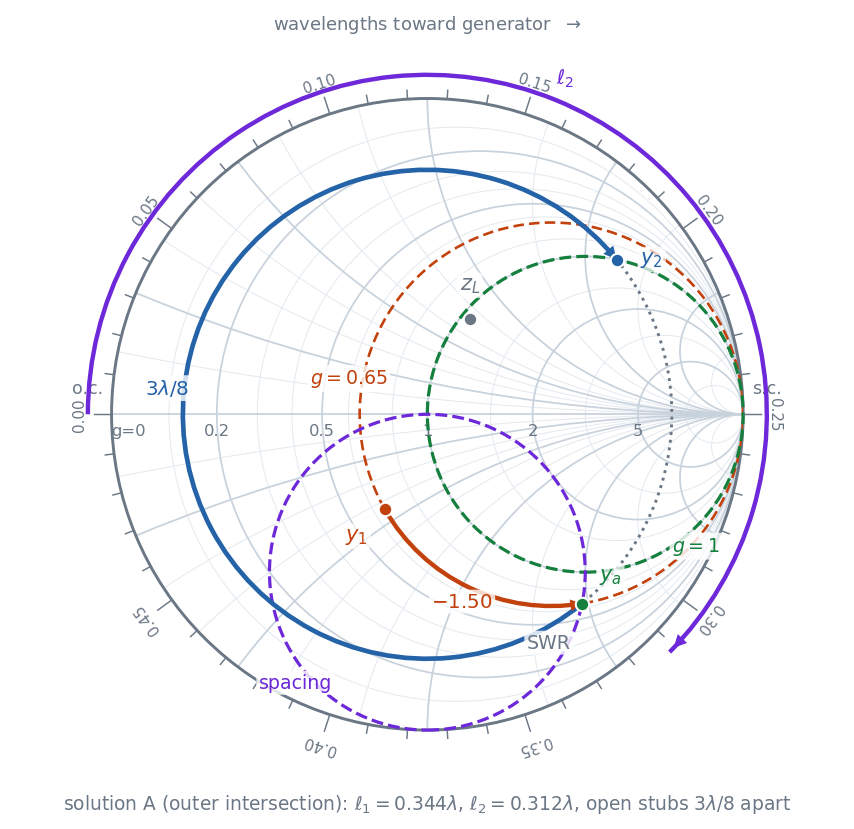
\includegraphics[width=0.495\textwidth]{figs/c2num_p19.png}\hfill
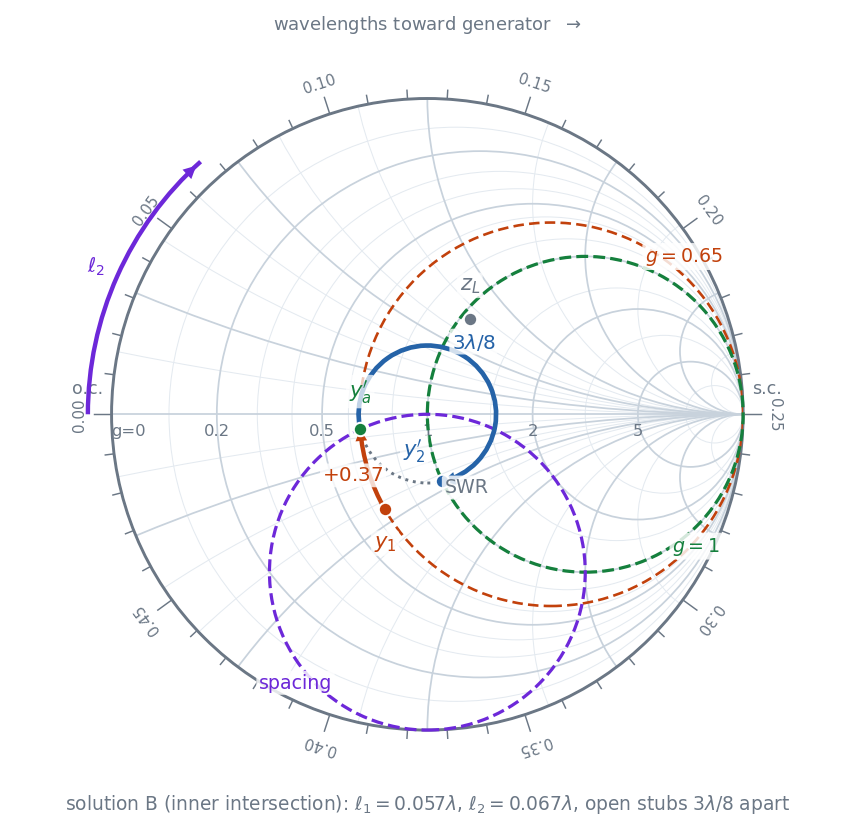
\includegraphics[width=0.495\textwidth]{figs/c2num_p19b.png}
\end{center}
{\footnotesize\color{sub} Problem 19 --- Smith chart construction, left: solution A, the outer intersection of the $g = 0.65$ circle with the spacing circle; right: solution B, the inner intersection of the $g = 0.65$ circle with the spacing circle.}

\figC{c2num_p19_line.png}{0.62\textwidth}
{\footnotesize\color{sub} Problem 19 --- line diagram of the matched network: shunt stubs across the line, lengths from the answer above.}

\figC{c2num_p19_ms.png}{0.62\textwidth}
{\footnotesize\color{sub} Problem 19 --- microstrip layout, top view: stubs as T-junctions off the main line, dimensions from the answer above.}

\penalty0\vspace{2pt}

%======================================================================
\Q{Problem 20 --- Double-stub shunt tuner}{\m{10}\m{2}\m{2}}
{\color{sub}\footnotesize \yr{\texttt{82 Ba}} \gap$\cdot$\gap $Z_0 = 100\,\Omega$}

\begin{asked}{\texttt{82 Ba} \ [10+2+2]}
An antenna at 10 GHz presents $\Gamma = |0.45|\angle 60^\circ$ on a $100\,\Omega$ line. Design a double-stub tuner, sketch the physical diagram using microstrips, and give the S-matrices before and after matching.
\end{asked}
\lead{Given}
\begin{itemize}
  \item $\Gamma_L = 0.450\angle 60.0^\circ$, $Z_0 = 100\,\Omega$ $\Rightarrow$ $Z_L = Z_0(1+\Gamma_L)/(1-\Gamma_L) = 105.98 + j103.58\,\Omega$.
  \item $f = 10\text{ GHz}$ $\Rightarrow$ $\lambda_0 = c/f = 30.0\text{ mm}$.
\end{itemize}
\lead{Step 1 --- normalise and plot $z_L$}
\begin{itemize}
  \item $z_L = Z_L/Z_0 = 105.98 + j103.58$ over $100$ $=1.06 + j1.04$.
  \item Plot it where the $r = 1.06$ circle cuts the $x = +1.04$ arc; it reads $0.167\lambda$ on the WTG scale.
  \item Dividers from centre to $z_L$ (the SWR-circle radius), laid on the radially scaled scales below the chart: $|\Gamma_L| = 0.450$ on \emph{refl.\ coeff.\ E or I}, $S = 2.64$ on \emph{SWR}. \textit{Check:} $(z_L-1)/(z_L+1) = 0.450\angle 60.0^\circ$, $(1+|\Gamma_L|)/(1-|\Gamma_L|) = 2.64$.
\end{itemize}
\lead{Step 2 --- convert to admittance}
\begin{itemize}
  \item Draw the diameter through $z_L$ and read the opposite intersection --- a $\lambda/4$ half-turn. On an immittance chart read the amber grid in place and skip this step.
  \item $y_L = 1/z_L = 0.48 - j0.47$, at $0.417\lambda$ on the WTG scale (exactly $0.25\lambda$ from $z_L$).
\end{itemize}
\lead{Step 3 --- the first stub is at the load}
\begin{itemize}
  \item No offset is specified, so stub 1 sits at the load and $y_1 = y_L = 0.48 - j0.47$.
\end{itemize}
\lead{Step 4 --- draw the spacing circle}
\begin{itemize}
  \item Rotate the $g=1$ circle $3\lambda/8$ \textbf{toward the load} (anticlockwise). Call the result the \textbf{spacing circle}.
  \item Any point on it is carried \emph{onto} $g=1$ by the $3\lambda/8$ of line between the two stubs --- which is exactly what stub 1 must aim for.
  \item Check the forbidden region first: matching needs $g_1 \le 1/\sin^2\beta d = 2.00$, and here $g_1 = 0.483$. \checkmark
\end{itemize}
\lead{Step 5 --- stub 1: slide along the constant-$g$ circle}
\begin{itemize}
  \item A shunt stub adds susceptance only, so the point can move \emph{only along its own $g = 0.483$ circle}.
  \item Follow that circle to where it cuts the spacing circle. It cuts twice, giving the two standard solutions (one chart each below):
  \begin{itemize}
    \item \textbf{Solution A} (outer intersection, nearer the rim): $y_a = 0.48 - j1.86$, so stub 1 must add $b_1 = -1.856 - (-0.472) = -1.384$.
    \item \textbf{Solution B} (inner intersection, nearer the centre): $y_a' = 0.48 - j0.14$, so $b_1' = +0.327$.
  \end{itemize}
  \item Read $\ell_1$ off the rim, starting at the short-circuit point ($y=\infty$, the right of the chart): $\ell_1 = 0.100\lambda$ (A) and $0.300\lambda$ (B).
\end{itemize}
\lead{Step 6 --- the $3\lambda/8$ of line between the stubs}
\begin{itemize}
  \item Swing a \emph{new} SWR circle through $y_a$ and rotate \textbf{clockwise} by $3\lambda/8$.
  \item By construction it lands on the $g=1$ circle: $y_2 = 1.00 + j2.77$ (A), $y_2' = 1.00 - j0.77$ (B).
\end{itemize}
\lead{Step 7 --- stub 2 cancels what is left}
\begin{itemize}
  \item Stub 2 supplies $b_2 = -2.773$ (A) or $+0.773$ (B), leaving $y_{in} = 1 + j0$, i.e. $Z_{in} = Z_0 = 100\,\Omega$. Matched.
  \item Off the rim from the short-circuit point ($y=\infty$, the right of the chart): $\ell_2 = 0.055\lambda$ (A) and $0.355\lambda$ (B).
\end{itemize}
\lead{Answer}
\begin{tabularx}{\linewidth}{@{}L{3.2cm}X X@{}}
\toprule
\hrow \thead{Quantity} & \thead{Solution A} & \thead{Solution B} \\
\midrule
Stub spacing $d$ & $3\lambda/8$ & $3\lambda/8$ \\
First stub from load & $0.000\lambda$ & $0.000\lambda$ \\
$y$ before stub 1 & $0.48 - j0.47$ & $0.48 - j0.47$ \\
Stub 1 susceptance $b_1$ & $-1.384$ & $+0.327$ \\
\textbf{Stub 1 length $\ell_1$} & $0.100\lambda$ & $0.300\lambda$ \\
$y$ after the spacing & $1.00 + j2.77$ & $1.00 - j0.77$ \\
Stub 2 susceptance $b_2$ & $-2.773$ & $+0.773$ \\
\textbf{Stub 2 length $\ell_2$} & $0.055\lambda$ & $0.355\lambda$ \\
\bottomrule
\end{tabularx}

\lead{Both are correct.} Quote either, but say which you chose. Solution A uses the shorter stubs here, which is the practical pick: less line at high VSWR means lower loss and wider bandwidth.
\lead{S-matrix before and after matching}
\begin{itemize}
  \item \textbf{Before} --- the bare load is a one-port, so $[S] = [\Gamma_L] = [0.450\angle 60.0^\circ]$, with $S = 2.64$.
  \item \textbf{After} --- the tuner makes $Z_{in} = Z_0$, so $S_{11} = S_{22} = 0$. The network is passive and reciprocal ($S_{12} = S_{21}$) and lossless, so unitarity forces $|S_{21}| = 1$:
\  \[ [S] = \begin{bmatrix} 0 & 1 \\ 1 & 0 \end{bmatrix} \quad \text{or} \quad \begin{bmatrix} 0 & e^{-j\theta} \\ e^{-j\theta} & 0 \end{bmatrix} \]
  \item Keeping the $e^{-j\theta}$ records the through-path electrical length; either form earns the marks if you say which you mean.
\end{itemize}
\lead{Microstrip realisation}
\begin{itemize}
  \item Take FR-4, $\epsilon_r = 4.4$, $h = 1.6\text{ mm}$. Hammerstad synthesis for $100\,\Omega$ gives $W/h = 0.44$, i.e. $W = 0.71\text{ mm}$, with $\epsilon_e = 3.02$.
  \item $\lambda_g = \lambda_0/\sqrt{\epsilon_e} = 17.2\text{ mm}$ at $10\text{ GHz}$, so:
  \begin{itemize}
    \item $\ell_1 = 0.100\lambda = 1.72\text{ mm}$.
    \item $\ell_2 = 0.055\lambda = 0.95\text{ mm}$.
    \item $d = 0.375\lambda = 6.47\text{ mm}$.
  \end{itemize}
  \item Draw the stubs as T-junctions off the $W$-wide main line. A shorted stub needs a plated via to the ground plane, drawn as a filled circle at the stub end.
  \item Shorten each open stub by the fringing allowance $\Delta\ell \approx 0.3h = 0.48\text{ mm}$.
\end{itemize}

\begin{center}
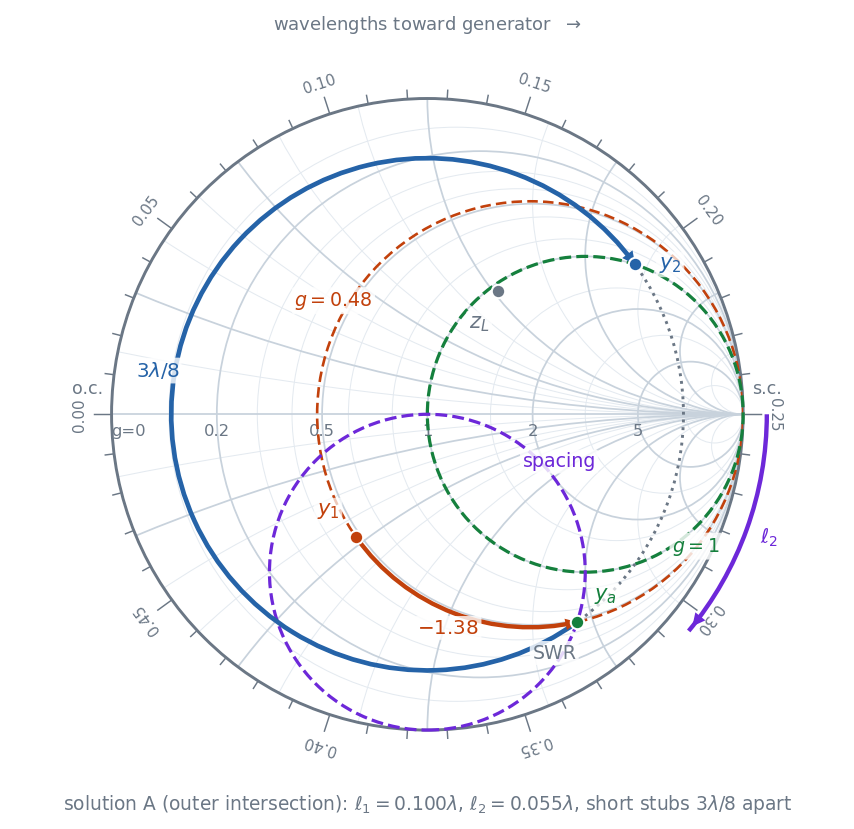
\includegraphics[width=0.495\textwidth]{figs/c2num_p20.png}\hfill
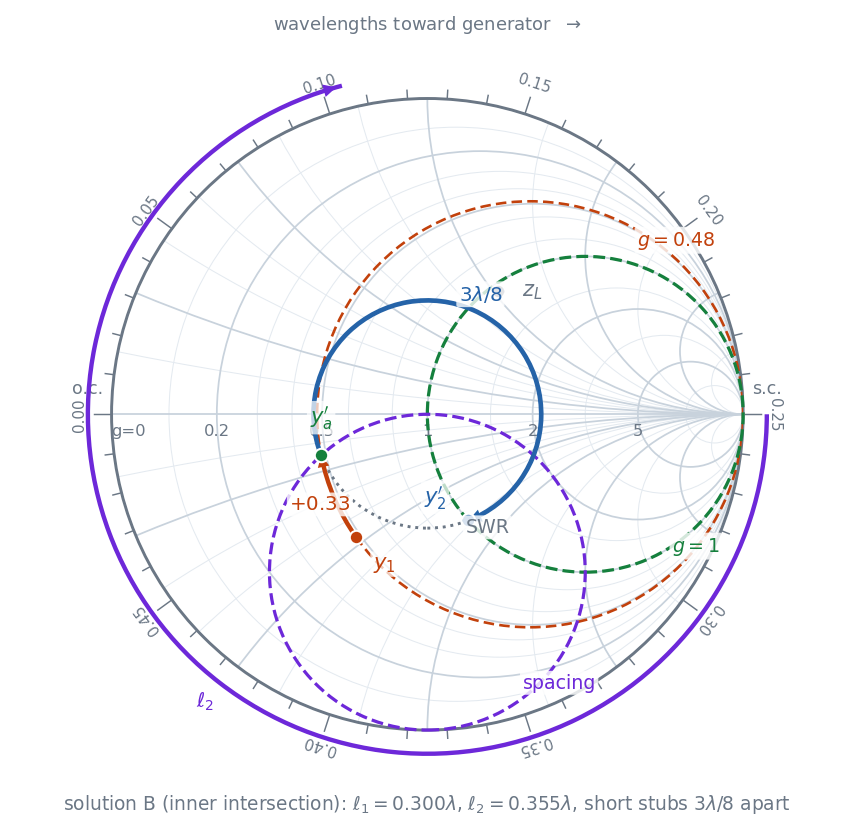
\includegraphics[width=0.495\textwidth]{figs/c2num_p20b.png}
\end{center}
{\footnotesize\color{sub} Problem 20 --- Smith chart construction, left: solution A, the outer intersection of the $g = 0.48$ circle with the spacing circle; right: solution B, the inner intersection of the $g = 0.48$ circle with the spacing circle.}

\figC{c2num_p20_line.png}{0.62\textwidth}
{\footnotesize\color{sub} Problem 20 --- line diagram of the matched network: shunt stubs across the line, lengths from the answer above.}

\figC{c2num_p20_ms.png}{0.62\textwidth}
{\footnotesize\color{sub} Problem 20 --- microstrip layout, top view: stubs as T-junctions off the main line, dimensions from the answer above.}

\penalty0\vspace{2pt}

%======================================================================
\Q{Problem 21 --- Double-stub shunt tuner}{\m{12}}
{\color{sub}\footnotesize \yr{\textbf{80 Ch}} \gap$\cdot$\gap $Z_0 = 100\,\Omega$}

\begin{asked}{\textbf{80 Ch} \ [12]}
Design a double-stub tuner ($3\lambda/8$ spacing) for $Z_L = 110+j110\,\Omega$ on a $100\,\Omega$ line: find the stub lengths and the spacing.
\end{asked}
\lead{Given}
\begin{itemize}
  \item $Z_L = 110.00 + j110.00\,\Omega$, $Z_0 = 100\,\Omega$.
\end{itemize}
\lead{Step 1 --- normalise and plot $z_L$}
\begin{itemize}
  \item $z_L = Z_L/Z_0 = 110.00 + j110.00$ over $100$ $=1.10 + j1.10$.
  \item Plot it where the $r = 1.10$ circle cuts the $x = +1.10$ arc; it reads $0.171\lambda$ on the WTG scale.
  \item Dividers from centre to $z_L$ (the SWR-circle radius), laid on the radially scaled scales below the chart: $|\Gamma_L| = 0.466$ on \emph{refl.\ coeff.\ E or I}, $S = 2.74$ on \emph{SWR}. \textit{Check:} $(z_L-1)/(z_L+1) = 0.466\angle 57.2^\circ$, $(1+|\Gamma_L|)/(1-|\Gamma_L|) = 2.74$.
\end{itemize}
\lead{Step 2 --- convert to admittance}
\begin{itemize}
  \item Draw the diameter through $z_L$ and read the opposite intersection --- a $\lambda/4$ half-turn. On an immittance chart read the amber grid in place and skip this step.
  \item $y_L = 1/z_L = 0.45 - j0.45$, at $0.421\lambda$ on the WTG scale (exactly $0.25\lambda$ from $z_L$).
\end{itemize}
\lead{Step 3 --- the first stub is at the load}
\begin{itemize}
  \item No offset is specified, so stub 1 sits at the load and $y_1 = y_L = 0.45 - j0.45$.
\end{itemize}
\lead{Step 4 --- draw the spacing circle}
\begin{itemize}
  \item Rotate the $g=1$ circle $3\lambda/8$ \textbf{toward the load} (anticlockwise). Call the result the \textbf{spacing circle}.
  \item Any point on it is carried \emph{onto} $g=1$ by the $3\lambda/8$ of line between the two stubs --- which is exactly what stub 1 must aim for.
  \item Check the forbidden region first: matching needs $g_1 \le 1/\sin^2\beta d = 2.00$, and here $g_1 = 0.455$. \checkmark
\end{itemize}
\lead{Step 5 --- stub 1: slide along the constant-$g$ circle}
\begin{itemize}
  \item A shunt stub adds susceptance only, so the point can move \emph{only along its own $g = 0.455$ circle}.
  \item Follow that circle to where it cuts the spacing circle. It cuts twice, giving the two standard solutions (one chart each below):
  \begin{itemize}
    \item \textbf{Solution A} (outer intersection, nearer the rim): $y_a = 0.45 - j1.84$, so stub 1 must add $b_1 = -1.838 - (-0.455) = -1.384$.
    \item \textbf{Solution B} (inner intersection, nearer the centre): $y_a' = 0.45 - j0.16$, so $b_1' = +0.293$.
  \end{itemize}
  \item Read $\ell_1$ off the rim, starting at the short-circuit point ($y=\infty$, the right of the chart): $\ell_1 = 0.100\lambda$ (A) and $0.295\lambda$ (B).
\end{itemize}
\lead{Step 6 --- the $3\lambda/8$ of line between the stubs}
\begin{itemize}
  \item Swing a \emph{new} SWR circle through $y_a$ and rotate \textbf{clockwise} by $3\lambda/8$.
  \item By construction it lands on the $g=1$ circle: $y_2 = 1.00 + j2.84$ (A), $y_2' = 1.00 - j0.84$ (B).
\end{itemize}
\lead{Step 7 --- stub 2 cancels what is left}
\begin{itemize}
  \item Stub 2 supplies $b_2 = -2.844$ (A) or $+0.844$ (B), leaving $y_{in} = 1 + j0$, i.e. $Z_{in} = Z_0 = 100\,\Omega$. Matched.
  \item Off the rim from the short-circuit point ($y=\infty$, the right of the chart): $\ell_2 = 0.054\lambda$ (A) and $0.362\lambda$ (B).
\end{itemize}
\lead{Answer}
\begin{tabularx}{\linewidth}{@{}L{3.2cm}X X@{}}
\toprule
\hrow \thead{Quantity} & \thead{Solution A} & \thead{Solution B} \\
\midrule
Stub spacing $d$ & $3\lambda/8$ & $3\lambda/8$ \\
First stub from load & $0.000\lambda$ & $0.000\lambda$ \\
$y$ before stub 1 & $0.45 - j0.45$ & $0.45 - j0.45$ \\
Stub 1 susceptance $b_1$ & $-1.384$ & $+0.293$ \\
\textbf{Stub 1 length $\ell_1$} & $0.100\lambda$ & $0.295\lambda$ \\
$y$ after the spacing & $1.00 + j2.84$ & $1.00 - j0.84$ \\
Stub 2 susceptance $b_2$ & $-2.844$ & $+0.844$ \\
\textbf{Stub 2 length $\ell_2$} & $0.054\lambda$ & $0.362\lambda$ \\
\bottomrule
\end{tabularx}

\lead{Both are correct.} Quote either, but say which you chose. Solution A uses the shorter stubs here, which is the practical pick: less line at high VSWR means lower loss and wider bandwidth.

\begin{center}
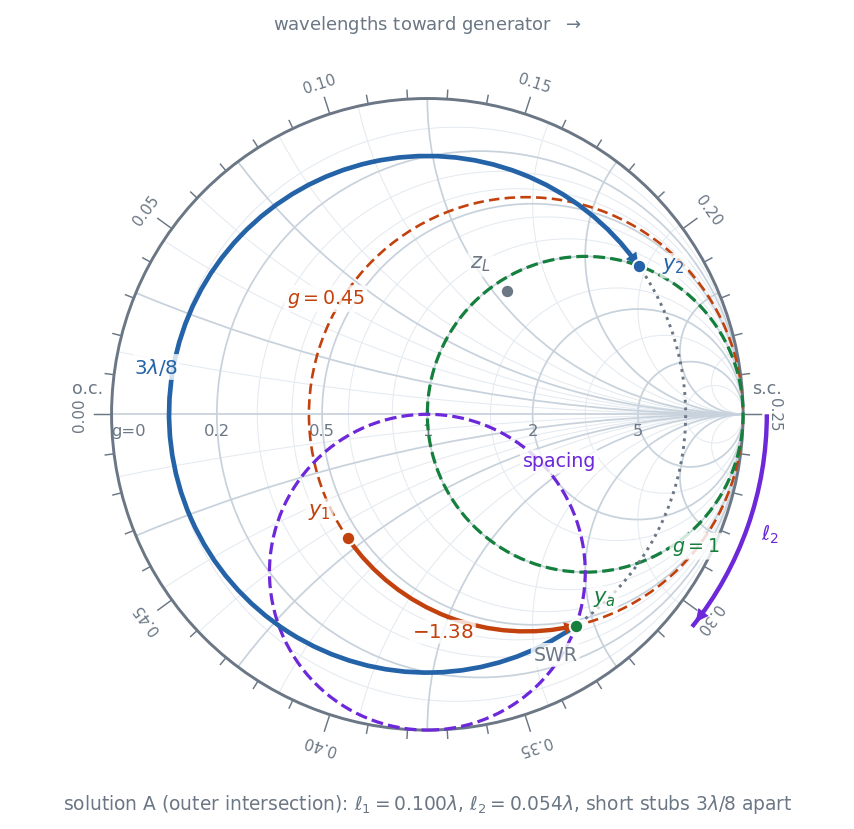
\includegraphics[width=0.495\textwidth]{figs/c2num_p21.png}\hfill
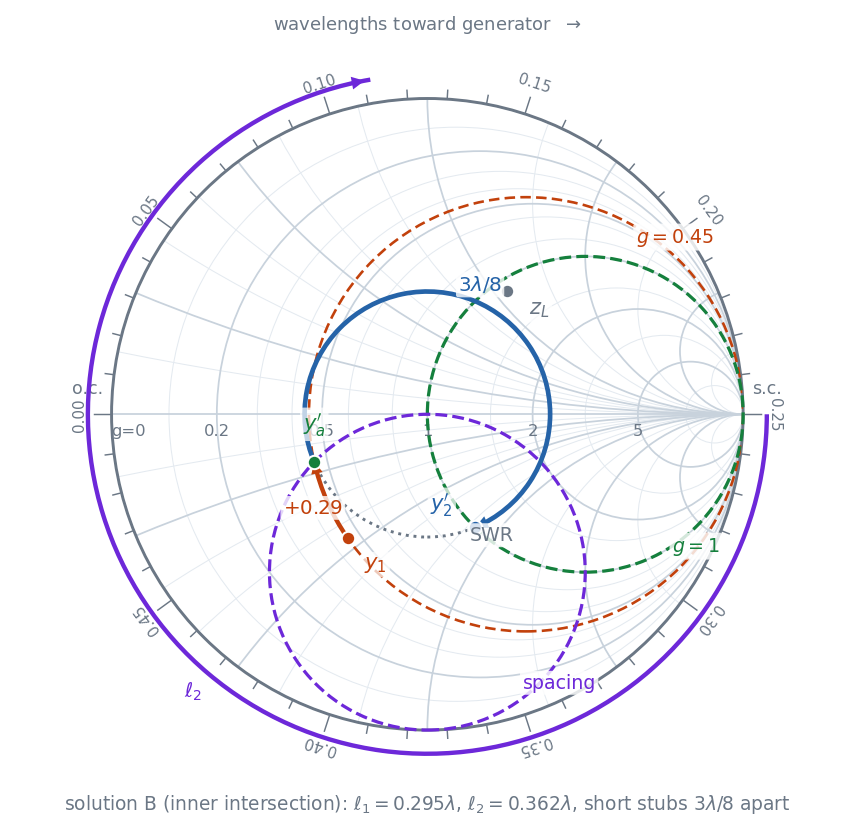
\includegraphics[width=0.495\textwidth]{figs/c2num_p21b.png}
\end{center}
{\footnotesize\color{sub} Problem 21 --- Smith chart construction, left: solution A, the outer intersection of the $g = 0.45$ circle with the spacing circle; right: solution B, the inner intersection of the $g = 0.45$ circle with the spacing circle.}

\figC{c2num_p21_line.png}{0.62\textwidth}
{\footnotesize\color{sub} Problem 21 --- line diagram of the matched network: shunt stubs across the line, lengths from the answer above.}

\figC{c2num_p21_coax.png}{0.69\textwidth}
{\footnotesize\color{sub} Problem 21 --- coaxial realisation, longitudinal section: each stub a coax tee off the main line; a shorting plate closes each stub.}

\penalty0\vspace{2pt}

%======================================================================
\Q{Problem 22 --- Double-stub shunt tuner}{\m{4}\m{6}}
{\color{sub}\footnotesize \yr{\textbf{78 Ch}} \gap$\cdot$\gap $Z_0 = 50\,\Omega$}

\begin{asked}{\textbf{78 Ch} \ [4+6]}
Explain the different impedance matching techniques and give the resulting S-matrix of a perfectly matched double-stub network.
\end{asked}
\lead{Given}
\begin{itemize}
  \item $Z_L = 100.00 + j50.00\,\Omega$, $Z_0 = 50\,\Omega$.
\end{itemize}
\lead{Step 1 --- normalise and plot $z_L$}
\begin{itemize}
  \item $z_L = Z_L/Z_0 = 100.00 + j50.00$ over $50$ $=2.00 + j1.00$.
  \item Plot it where the $r = 2.00$ circle cuts the $x = +1.00$ arc; it reads $0.213\lambda$ on the WTG scale.
  \item Dividers from centre to $z_L$ (the SWR-circle radius), laid on the radially scaled scales below the chart: $|\Gamma_L| = 0.447$ on \emph{refl.\ coeff.\ E or I}, $S = 2.62$ on \emph{SWR}. \textit{Check:} $(z_L-1)/(z_L+1) = 0.447\angle 26.6^\circ$, $(1+|\Gamma_L|)/(1-|\Gamma_L|) = 2.62$.
\end{itemize}
\lead{Step 2 --- convert to admittance}
\begin{itemize}
  \item Draw the diameter through $z_L$ and read the opposite intersection --- a $\lambda/4$ half-turn. On an immittance chart read the amber grid in place and skip this step.
  \item $y_L = 1/z_L = 0.40 - j0.20$, at $0.463\lambda$ on the WTG scale (exactly $0.25\lambda$ from $z_L$).
\end{itemize}
\lead{Step 3 --- the first stub is at the load}
\begin{itemize}
  \item No offset is specified, so stub 1 sits at the load and $y_1 = y_L = 0.40 - j0.20$.
\end{itemize}
\lead{Step 4 --- draw the spacing circle}
\begin{itemize}
  \item Rotate the $g=1$ circle $3\lambda/8$ \textbf{toward the load} (anticlockwise). Call the result the \textbf{spacing circle}.
  \item Any point on it is carried \emph{onto} $g=1$ by the $3\lambda/8$ of line between the two stubs --- which is exactly what stub 1 must aim for.
  \item Check the forbidden region first: matching needs $g_1 \le 1/\sin^2\beta d = 2.00$, and here $g_1 = 0.400$. \checkmark
\end{itemize}
\lead{Step 5 --- stub 1: slide along the constant-$g$ circle}
\begin{itemize}
  \item A shunt stub adds susceptance only, so the point can move \emph{only along its own $g = 0.400$ circle}.
  \item Follow that circle to where it cuts the spacing circle. It cuts twice, giving the two standard solutions (one chart each below):
  \begin{itemize}
    \item \textbf{Solution A} (outer intersection, nearer the rim): $y_a = 0.40 - j1.80$, so stub 1 must add $b_1 = -1.800 - (-0.200) = -1.600$.
    \item \textbf{Solution B} (inner intersection, nearer the centre): $y_a' = 0.40 - j0.20$, so $b_1' = +0.000$.
  \end{itemize}
  \item Read $\ell_1$ off the rim, starting at the short-circuit point ($y=\infty$, the right of the chart): $\ell_1 = 0.089\lambda$ (A) and $0.250\lambda$ (B).
\end{itemize}
\lead{Step 6 --- the $3\lambda/8$ of line between the stubs}
\begin{itemize}
  \item Swing a \emph{new} SWR circle through $y_a$ and rotate \textbf{clockwise} by $3\lambda/8$.
  \item By construction it lands on the $g=1$ circle: $y_2 = 1.00 + j3.00$ (A), $y_2' = 1.00 - j1.00$ (B).
\end{itemize}
\lead{Step 7 --- stub 2 cancels what is left}
\begin{itemize}
  \item Stub 2 supplies $b_2 = -3.000$ (A) or $+1.000$ (B), leaving $y_{in} = 1 + j0$, i.e. $Z_{in} = Z_0 = 50\,\Omega$. Matched.
  \item Off the rim from the short-circuit point ($y=\infty$, the right of the chart): $\ell_2 = 0.051\lambda$ (A) and $0.375\lambda$ (B).
\end{itemize}
\lead{Answer}
\begin{tabularx}{\linewidth}{@{}L{3.2cm}X X@{}}
\toprule
\hrow \thead{Quantity} & \thead{Solution A} & \thead{Solution B} \\
\midrule
Stub spacing $d$ & $3\lambda/8$ & $3\lambda/8$ \\
First stub from load & $0.000\lambda$ & $0.000\lambda$ \\
$y$ before stub 1 & $0.40 - j0.20$ & $0.40 - j0.20$ \\
Stub 1 susceptance $b_1$ & $-1.600$ & $+0.000$ \\
\textbf{Stub 1 length $\ell_1$} & $0.089\lambda$ & $0.250\lambda$ \\
$y$ after the spacing & $1.00 + j3.00$ & $1.00 - j1.00$ \\
Stub 2 susceptance $b_2$ & $-3.000$ & $+1.000$ \\
\textbf{Stub 2 length $\ell_2$} & $0.051\lambda$ & $0.375\lambda$ \\
\bottomrule
\end{tabularx}

\lead{Both are correct.} Quote either, but say which you chose. Solution A uses the shorter stubs here, which is the practical pick: less line at high VSWR means lower loss and wider bandwidth.
\lead{S-matrix before and after matching}
\begin{itemize}
  \item \textbf{Before} --- the bare load is a one-port, so $[S] = [\Gamma_L] = [0.447\angle 26.6^\circ]$, with $S = 2.62$.
  \item \textbf{After} --- the tuner makes $Z_{in} = Z_0$, so $S_{11} = S_{22} = 0$. The network is passive and reciprocal ($S_{12} = S_{21}$) and lossless, so unitarity forces $|S_{21}| = 1$:
\  \[ [S] = \begin{bmatrix} 0 & 1 \\ 1 & 0 \end{bmatrix} \quad \text{or} \quad \begin{bmatrix} 0 & e^{-j\theta} \\ e^{-j\theta} & 0 \end{bmatrix} \]
  \item Keeping the $e^{-j\theta}$ records the through-path electrical length; either form earns the marks if you say which you mean.
\end{itemize}
\lead{Theory half} The comparison of matching techniques and the advantages of double-stub over single-stub tuning are in $\S$2.5; the design steps and the forbidden region are in $\S$2.7. The worked example above supplies the ``+Eg'' the paper asks for.

\begin{center}
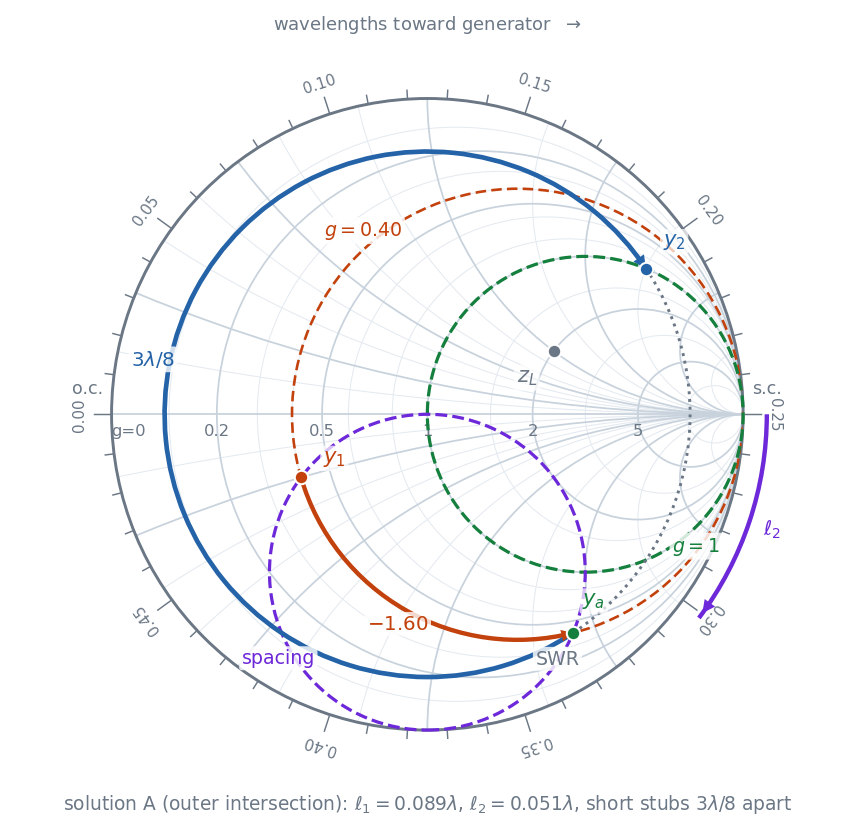
\includegraphics[width=0.495\textwidth]{figs/c2num_p22.png}\hfill
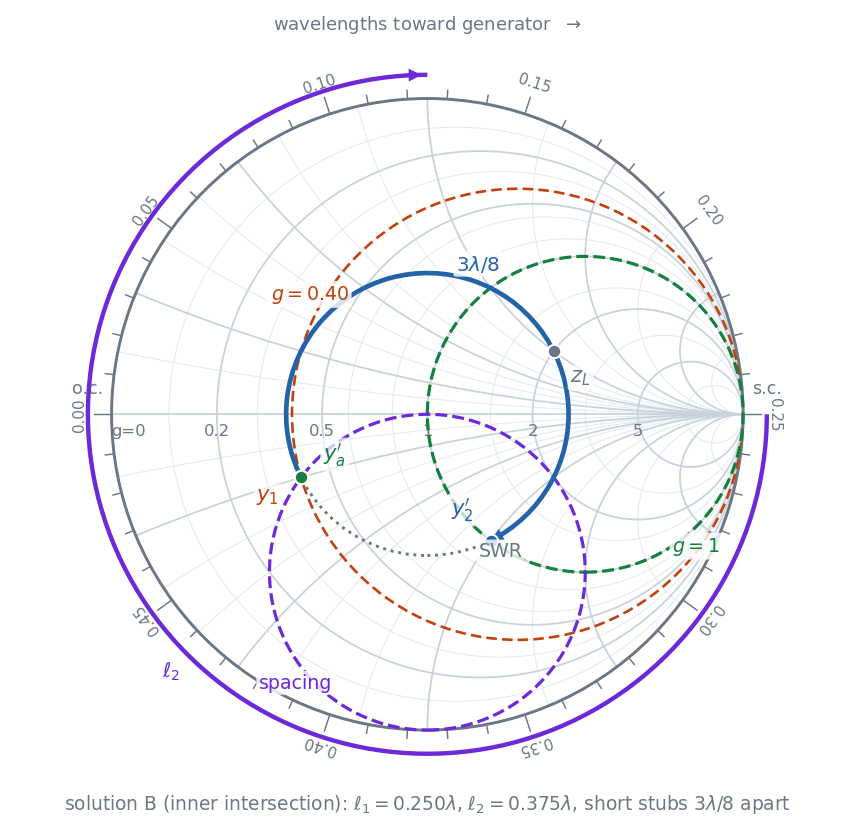
\includegraphics[width=0.495\textwidth]{figs/c2num_p22b.png}
\end{center}
{\footnotesize\color{sub} Problem 22 --- Smith chart construction, left: solution A, the outer intersection of the $g = 0.40$ circle with the spacing circle; right: solution B, the inner intersection of the $g = 0.40$ circle with the spacing circle.}

\figC{c2num_p22_line.png}{0.62\textwidth}
{\footnotesize\color{sub} Problem 22 --- line diagram of the matched network: shunt stubs across the line, lengths from the answer above.}

\figC{c2num_p22_coax.png}{0.69\textwidth}
{\footnotesize\color{sub} Problem 22 --- coaxial realisation, longitudinal section: each stub a coax tee off the main line; a shorting plate closes each stub.}

\penalty0\vspace{2pt}

%======================================================================
\Q{Problem 23 --- Double-stub shunt tuner}{\m{2}\m{8}}
{\color{sub}\footnotesize \yr{\textbf{77 Ch}} \gap$\cdot$\gap $Z_0 = 50\,\Omega$}

\begin{asked}{\textbf{77 Ch} \ [2+8]}
Sketch a double-stub perfectly matched network using microstrip and prepare its S-matrix.
\end{asked}
\lead{Given}
\begin{itemize}
  \item $Z_L = 25.00 - j40.00\,\Omega$, $Z_0 = 50\,\Omega$.
\end{itemize}
\lead{Step 1 --- normalise and plot $z_L$}
\begin{itemize}
  \item $z_L = Z_L/Z_0 = 25.00 - j40.00$ over $50$ $=0.50 - j0.80$.
  \item Plot it where the $r = 0.50$ circle cuts the $x = -0.80$ arc; it reads $0.380\lambda$ on the WTG scale.
  \item Dividers from centre to $z_L$ (the SWR-circle radius), laid on the radially scaled scales below the chart: $|\Gamma_L| = 0.555$ on \emph{refl.\ coeff.\ E or I}, $S = 3.49$ on \emph{SWR}. \textit{Check:} $(z_L-1)/(z_L+1) = 0.555\angle -93.9^\circ$, $(1+|\Gamma_L|)/(1-|\Gamma_L|) = 3.49$.
\end{itemize}
\lead{Step 2 --- convert to admittance}
\begin{itemize}
  \item Draw the diameter through $z_L$ and read the opposite intersection --- a $\lambda/4$ half-turn. On an immittance chart read the amber grid in place and skip this step.
  \item $y_L = 1/z_L = 0.56 + j0.90$, at $0.130\lambda$ on the WTG scale (exactly $0.25\lambda$ from $z_L$).
\end{itemize}
\lead{Step 3 --- the first stub is at the load}
\begin{itemize}
  \item No offset is specified, so stub 1 sits at the load and $y_1 = y_L = 0.56 + j0.90$.
\end{itemize}
\lead{Step 4 --- draw the spacing circle}
\begin{itemize}
  \item Rotate the $g=1$ circle $3\lambda/8$ \textbf{toward the load} (anticlockwise). Call the result the \textbf{spacing circle}.
  \item Any point on it is carried \emph{onto} $g=1$ by the $3\lambda/8$ of line between the two stubs --- which is exactly what stub 1 must aim for.
  \item Check the forbidden region first: matching needs $g_1 \le 1/\sin^2\beta d = 2.00$, and here $g_1 = 0.562$. \checkmark
\end{itemize}
\lead{Step 5 --- stub 1: slide along the constant-$g$ circle}
\begin{itemize}
  \item A shunt stub adds susceptance only, so the point can move \emph{only along its own $g = 0.562$ circle}.
  \item Follow that circle to where it cuts the spacing circle. It cuts twice, giving the two standard solutions (one chart each below):
  \begin{itemize}
    \item \textbf{Solution A} (outer intersection, nearer the rim): $y_a = 0.56 - j1.90$, so stub 1 must add $b_1 = -1.899 - (0.899) = -2.798$.
    \item \textbf{Solution B} (inner intersection, nearer the centre): $y_a' = 0.56 - j0.10$, so $b_1' = -1.000$.
  \end{itemize}
  \item Read $\ell_1$ off the rim, starting at the open-circuit point ($y=0$, the left of the chart): $\ell_1 = 0.305\lambda$ (A) and $0.375\lambda$ (B).
\end{itemize}
\lead{Step 6 --- the $3\lambda/8$ of line between the stubs}
\begin{itemize}
  \item Swing a \emph{new} SWR circle through $y_a$ and rotate \textbf{clockwise} by $3\lambda/8$.
  \item By construction it lands on the $g=1$ circle: $y_2 = 1.00 + j2.60$ (A), $y_2' = 1.00 - j0.60$ (B).
\end{itemize}
\lead{Step 7 --- stub 2 cancels what is left}
\begin{itemize}
  \item Stub 2 supplies $b_2 = -2.600$ (A) or $+0.600$ (B), leaving $y_{in} = 1 + j0$, i.e. $Z_{in} = Z_0 = 50\,\Omega$. Matched.
  \item Off the rim from the open-circuit point ($y=0$, the left of the chart): $\ell_2 = 0.308\lambda$ (A) and $0.086\lambda$ (B).
\end{itemize}
\lead{Answer}
\begin{tabularx}{\linewidth}{@{}L{3.2cm}X X@{}}
\toprule
\hrow \thead{Quantity} & \thead{Solution A} & \thead{Solution B} \\
\midrule
Stub spacing $d$ & $3\lambda/8$ & $3\lambda/8$ \\
First stub from load & $0.000\lambda$ & $0.000\lambda$ \\
$y$ before stub 1 & $0.56 + j0.90$ & $0.56 + j0.90$ \\
Stub 1 susceptance $b_1$ & $-2.798$ & $-1.000$ \\
\textbf{Stub 1 length $\ell_1$} & $0.305\lambda$ & $0.375\lambda$ \\
$y$ after the spacing & $1.00 + j2.60$ & $1.00 - j0.60$ \\
Stub 2 susceptance $b_2$ & $-2.600$ & $+0.600$ \\
\textbf{Stub 2 length $\ell_2$} & $0.308\lambda$ & $0.086\lambda$ \\
\bottomrule
\end{tabularx}

\lead{Both are correct.} Quote either, but say which you chose. Solution B uses the shorter stubs here, which is the practical pick: less line at high VSWR means lower loss and wider bandwidth.
\lead{S-matrix before and after matching}
\begin{itemize}
  \item \textbf{Before} --- the bare load is a one-port, so $[S] = [\Gamma_L] = [0.555\angle -93.9^\circ]$, with $S = 3.49$.
  \item \textbf{After} --- the tuner makes $Z_{in} = Z_0$, so $S_{11} = S_{22} = 0$. The network is passive and reciprocal ($S_{12} = S_{21}$) and lossless, so unitarity forces $|S_{21}| = 1$:
\  \[ [S] = \begin{bmatrix} 0 & 1 \\ 1 & 0 \end{bmatrix} \quad \text{or} \quad \begin{bmatrix} 0 & e^{-j\theta} \\ e^{-j\theta} & 0 \end{bmatrix} \]
  \item Keeping the $e^{-j\theta}$ records the through-path electrical length; either form earns the marks if you say which you mean.
\end{itemize}
\lead{Microstrip realisation}
\begin{itemize}
  \item Take FR-4, $\epsilon_r = 4.4$, $h = 1.6\text{ mm}$. Hammerstad synthesis for $50\,\Omega$ gives $W/h = 1.91$, i.e. $W = 3.06\text{ mm}$, with $\epsilon_e = 3.33$.
  \item No frequency is given, so leave the answers in wavelengths; multiply by $\lambda_g = \lambda_0/\sqrt{\epsilon_e}$ once $f$ is fixed.
  \item Draw the stubs as T-junctions off the $W$-wide main line. Open stubs are plain truncated strips (no via needed) --- which is why open stubs are preferred in microstrip.
  \item Shorten each open stub by the fringing allowance $\Delta\ell \approx 0.3h = 0.48\text{ mm}$.
\end{itemize}
\lead{Theory half} The comparison of matching techniques and the advantages of double-stub over single-stub tuning are in $\S$2.5; the design steps and the forbidden region are in $\S$2.7. The worked example above supplies the ``+Eg'' the paper asks for.

\begin{center}
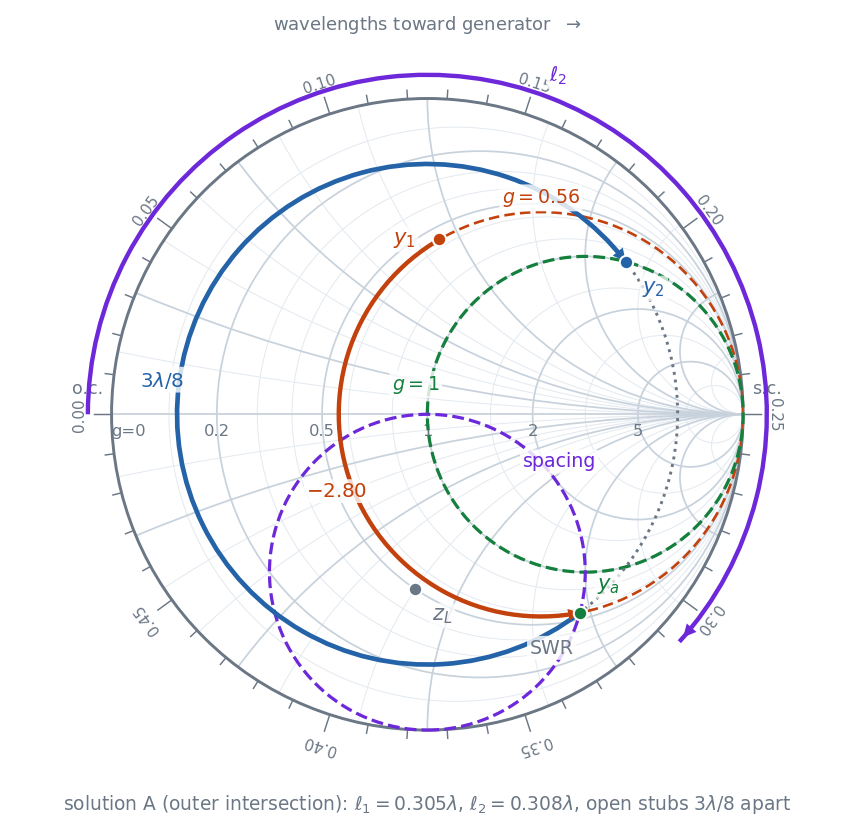
\includegraphics[width=0.495\textwidth]{figs/c2num_p23.png}\hfill
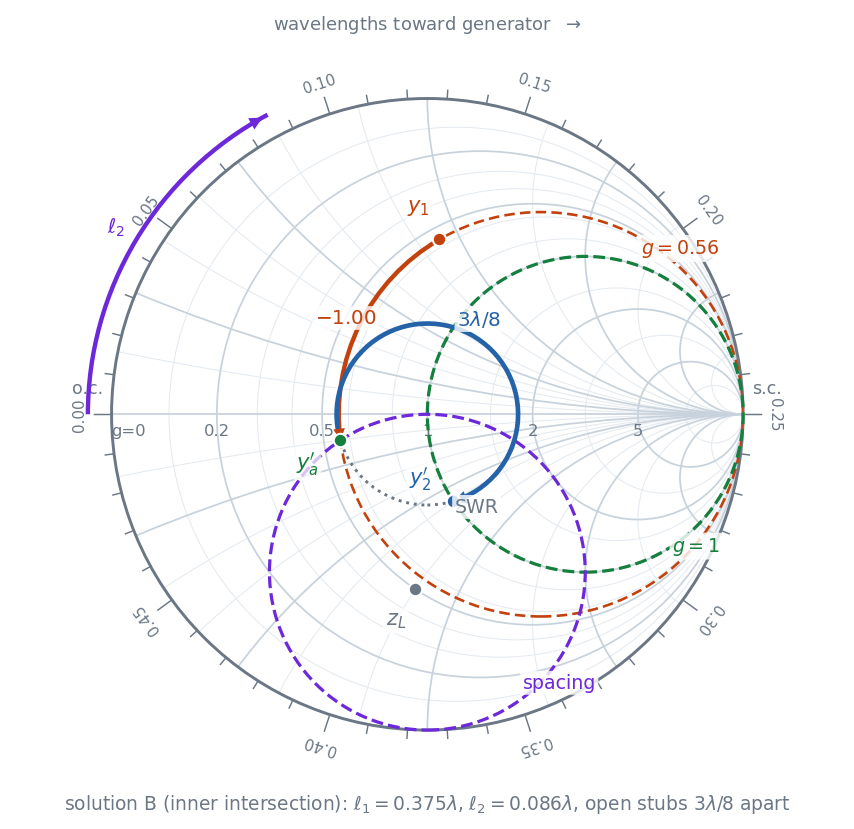
\includegraphics[width=0.495\textwidth]{figs/c2num_p23b.png}
\end{center}
{\footnotesize\color{sub} Problem 23 --- Smith chart construction, left: solution A, the outer intersection of the $g = 0.56$ circle with the spacing circle; right: solution B, the inner intersection of the $g = 0.56$ circle with the spacing circle.}

\figC{c2num_p23_line.png}{0.62\textwidth}
{\footnotesize\color{sub} Problem 23 --- line diagram of the matched network: shunt stubs across the line, lengths from the answer above.}

\figC{c2num_p23_ms.png}{0.62\textwidth}
{\footnotesize\color{sub} Problem 23 --- microstrip layout, top view: stubs as T-junctions off the main line, dimensions from the answer above.}

\penalty0\vspace{2pt}

%======================================================================
\Q{Problem 24 --- Double-stub shunt tuner}{\m{2}\m{8}}
{\color{sub}\footnotesize \yr{74 Ma} \gap$\cdot$\gap $Z_0 = 50\,\Omega$}

\begin{asked}{74 Ma \ [2+8]}
State the advantages of double-stub matching over single-stub matching, and give the steps for matching a load with a double-stub network with an example, using the provided Smith chart.
\end{asked}
\lead{Given}
\begin{itemize}
  \item $Z_L = 30.00 + j40.00\,\Omega$, $Z_0 = 50\,\Omega$.
\end{itemize}
\lead{Step 1 --- normalise and plot $z_L$}
\begin{itemize}
  \item $z_L = Z_L/Z_0 = 30.00 + j40.00$ over $50$ $=0.60 + j0.80$.
  \item Plot it where the $r = 0.60$ circle cuts the $x = +0.80$ arc; it reads $0.125\lambda$ on the WTG scale.
  \item Dividers from centre to $z_L$ (the SWR-circle radius), laid on the radially scaled scales below the chart: $|\Gamma_L| = 0.500$ on \emph{refl.\ coeff.\ E or I}, $S = 3.00$ on \emph{SWR}. \textit{Check:} $(z_L-1)/(z_L+1) = 0.500\angle 90.0^\circ$, $(1+|\Gamma_L|)/(1-|\Gamma_L|) = 3.00$.
\end{itemize}
\lead{Step 2 --- convert to admittance}
\begin{itemize}
  \item Draw the diameter through $z_L$ and read the opposite intersection --- a $\lambda/4$ half-turn. On an immittance chart read the amber grid in place and skip this step.
  \item $y_L = 1/z_L = 0.60 - j0.80$, at $0.375\lambda$ on the WTG scale (exactly $0.25\lambda$ from $z_L$).
\end{itemize}
\lead{Step 3 --- the first stub is at the load}
\begin{itemize}
  \item No offset is specified, so stub 1 sits at the load and $y_1 = y_L = 0.60 - j0.80$.
\end{itemize}
\lead{Step 4 --- draw the spacing circle}
\begin{itemize}
  \item Rotate the $g=1$ circle $3\lambda/8$ \textbf{toward the load} (anticlockwise). Call the result the \textbf{spacing circle}.
  \item Any point on it is carried \emph{onto} $g=1$ by the $3\lambda/8$ of line between the two stubs --- which is exactly what stub 1 must aim for.
  \item Check the forbidden region first: matching needs $g_1 \le 1/\sin^2\beta d = 2.00$, and here $g_1 = 0.600$. \checkmark
\end{itemize}
\lead{Step 5 --- stub 1: slide along the constant-$g$ circle}
\begin{itemize}
  \item A shunt stub adds susceptance only, so the point can move \emph{only along its own $g = 0.600$ circle}.
  \item Follow that circle to where it cuts the spacing circle. It cuts twice, giving the two standard solutions (one chart each below):
  \begin{itemize}
    \item \textbf{Solution A} (outer intersection, nearer the rim): $y_a = 0.60 - j1.92$, so stub 1 must add $b_1 = -1.917 - (-0.800) = -1.117$.
    \item \textbf{Solution B} (inner intersection, nearer the centre): $y_a' = 0.60 - j0.08$, so $b_1' = +0.717$.
  \end{itemize}
  \item Read $\ell_1$ off the rim, starting at the short-circuit point ($y=\infty$, the right of the chart): $\ell_1 = 0.116\lambda$ (A) and $0.349\lambda$ (B).
\end{itemize}
\lead{Step 6 --- the $3\lambda/8$ of line between the stubs}
\begin{itemize}
  \item Swing a \emph{new} SWR circle through $y_a$ and rotate \textbf{clockwise} by $3\lambda/8$.
  \item By construction it lands on the $g=1$ circle: $y_2 = 1.00 + j2.53$ (A), $y_2' = 1.00 - j0.53$ (B).
\end{itemize}
\lead{Step 7 --- stub 2 cancels what is left}
\begin{itemize}
  \item Stub 2 supplies $b_2 = -2.528$ (A) or $+0.528$ (B), leaving $y_{in} = 1 + j0$, i.e. $Z_{in} = Z_0 = 50\,\Omega$. Matched.
  \item Off the rim from the short-circuit point ($y=\infty$, the right of the chart): $\ell_2 = 0.060\lambda$ (A) and $0.327\lambda$ (B).
\end{itemize}
\lead{Answer}
\begin{tabularx}{\linewidth}{@{}L{3.2cm}X X@{}}
\toprule
\hrow \thead{Quantity} & \thead{Solution A} & \thead{Solution B} \\
\midrule
Stub spacing $d$ & $3\lambda/8$ & $3\lambda/8$ \\
First stub from load & $0.000\lambda$ & $0.000\lambda$ \\
$y$ before stub 1 & $0.60 - j0.80$ & $0.60 - j0.80$ \\
Stub 1 susceptance $b_1$ & $-1.117$ & $+0.717$ \\
\textbf{Stub 1 length $\ell_1$} & $0.116\lambda$ & $0.349\lambda$ \\
$y$ after the spacing & $1.00 + j2.53$ & $1.00 - j0.53$ \\
Stub 2 susceptance $b_2$ & $-2.528$ & $+0.528$ \\
\textbf{Stub 2 length $\ell_2$} & $0.060\lambda$ & $0.327\lambda$ \\
\bottomrule
\end{tabularx}

\lead{Both are correct.} Quote either, but say which you chose. Solution A uses the shorter stubs here, which is the practical pick: less line at high VSWR means lower loss and wider bandwidth.
\lead{Theory half} The comparison of matching techniques and the advantages of double-stub over single-stub tuning are in $\S$2.5; the design steps and the forbidden region are in $\S$2.7. The worked example above supplies the ``+Eg'' the paper asks for.

\begin{center}
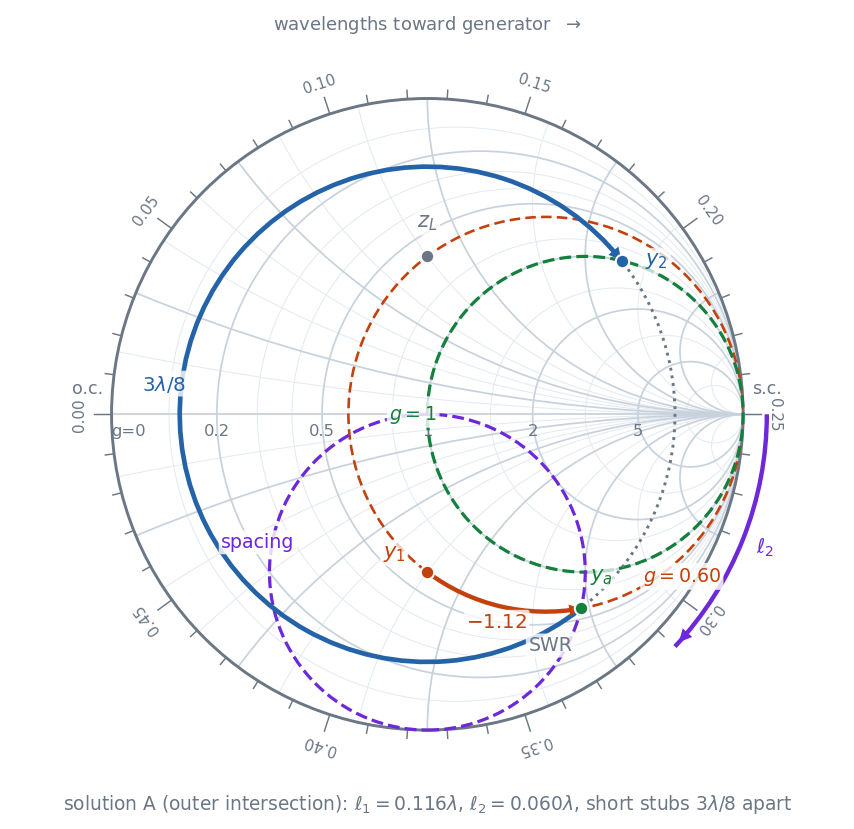
\includegraphics[width=0.495\textwidth]{figs/c2num_p24.png}\hfill
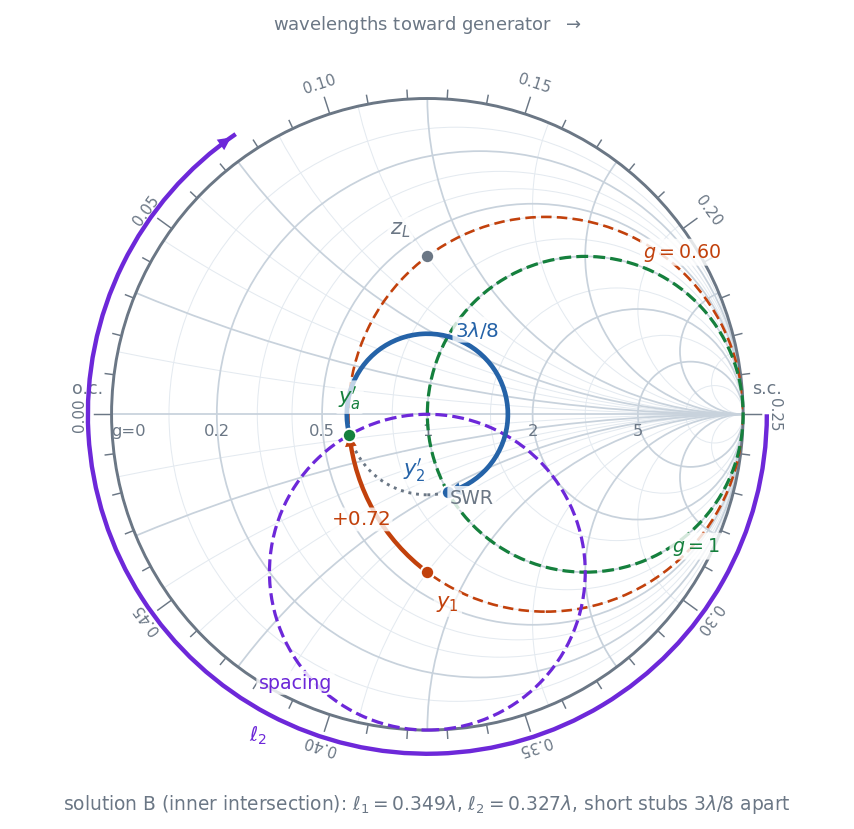
\includegraphics[width=0.495\textwidth]{figs/c2num_p24b.png}
\end{center}
{\footnotesize\color{sub} Problem 24 --- Smith chart construction, left: solution A, the outer intersection of the $g = 0.60$ circle with the spacing circle; right: solution B, the inner intersection of the $g = 0.60$ circle with the spacing circle.}

\figC{c2num_p24_line.png}{0.62\textwidth}
{\footnotesize\color{sub} Problem 24 --- line diagram of the matched network: shunt stubs across the line, lengths from the answer above.}

\figC{c2num_p24_coax.png}{0.69\textwidth}
{\footnotesize\color{sub} Problem 24 --- coaxial realisation, longitudinal section: each stub a coax tee off the main line; a shorting plate closes each stub.}

\penalty0\vspace{2pt}

